\documentclass[12pt]{extarticle}

%%%% paramètres généraux
%%%% french character
\usepackage[french]{babel}
\usepackage[T1]{fontenc}
\usepackage[utf8]{inputenc}

%%%% useful packages
\usepackage[a4paper, left=1.3cm, right=1.3cm, top=2.2cm, bottom=2.3cm]{geometry}
\usepackage{subcaption} % for figure caption
\usepackage{graphicx} % image
\usepackage{tabularx} % table
\usepackage[table]{xcolor} % color in table
\usepackage{amsmath} % math
\usepackage{amssymb} % bold math
\usepackage{wasysym} % integral
\usepackage[many]{tcolorbox} % colored box
\usepackage{fancyhdr} % headers
\usepackage{enumitem} % for bullet in itemize
\usepackage[colorlinks=true,linkcolor=black,citecolor=black,filecolor=black,urlcolor=black]{hyperref} % for link
\usepackage{accents} % for complex notation
\usepackage[european, straightvoltages, RPvoltages]{circuitikz} % for electronic circuit
\usepackage{multicol} % to use several columns
\usepackage{fontawesome} % awesome icons
\usepackage{ifthen} % for loop and boolean in commands
\usepackage{pdfpages} % to include pdf
\usepackage{wrapfig} % to wrap text around figures
\usepackage{chemfig} % to draw chemistry formula
\usepackage{chemist} % surtout pour chemform
\usepackage{multirow} % for vertically merged cells
\usepackage{makecell} % to format cell in tables
\usepackage{physics} % for derivatives, braket, etc.
\usepackage{esvect} % for large vectors
\usepackage{listings} % for code
\usepackage{dashundergaps} % for automatic text to fill
% dyslexia friendly font (need to be compiled in xetex)
%\usepackage{fontspec}
%\setmainfont{OpenDyslexic}
\usepackage{tikz}
\usepackage{pgfplots}
\usepackage[framemethod=tikz]{mdframed} %pour les boîtes

%%%% settings
\setlength{\parskip}{0cm}
\setlength{\parindent}{0cm}
\renewcommand{\baselinestretch}{1}
\setcounter{tocdepth}{2}
\renewcommand{\thesection}{\textcolor{red}{\Roman{section}}}
\renewcommand{\thesubsection}{\textcolor{red}{\Roman{section}.\arabic{subsection}}}

%%%% tikz configuration
\usetikzlibrary{babel}
\tikzset{>=latex}
\usetikzlibrary{shadows}
\usetikzlibrary{backgrounds}



%%%% header
\renewcommand{\headrulewidth}{0.4pt}
\setlength{\headheight}{22.50113pt}


%%%% Table
\renewcommand{\tabularxcolumn}[1]{m{#1}}
\setlength{\extrarowheight}{8pt}


%%%% Chemfig configuration
\setchemfig{
  atom sep=20pt,
  bond style={line width=1pt},
  angle increment=30
}


%%%% dashundergaps configuration
\dashundergapssetup{
  gap-numbers = false,
  gap-format = dot,
  gap-widen,
  gap-extend-percent
}

%%%% quelques commandes
%%%%%%%%%%%%%%%%%%%%%%%%%%%%%%%%%%%%%%%%%%%%%%%%%%%%%%%%%%%%%%%%%%%%%%%%%%
%%%% quelque couleurs
\definecolor{vertSombre} {RGB}{  0,  92,  46}
\definecolor{cyanSombre} {RGB}{  0, 140, 128}
\definecolor{jauneSombre}{RGB}{138, 103,   0}
\definecolor{jauneClair} {RGB}{218, 173,   0}
\definecolor{rougeSombre}{RGB}{148,  31,   0}
\definecolor{rougeClair} {RGB}{224,  39,  34}
\definecolor{couleurtitre}{RGB}{255,  255,  255}
\definecolor{exef}{RGB}{210,210,210}
\definecolor{propositiono}{RGB}{109,109,109}

%%% quelques couleurs dérivées des couleurs choisie
\newcommand{\couleurCorrection}{couleurPrincipale!60!black}
\newcommand{\couleurExercice}{couleurPrincipale!75!black}

%%%% rectangle coloré
\newcommand\rectangle[3]{%
  \shorthandoff{;}
  \tikz \node (rect) [draw, fill, color=#1,
              minimum width=#2,
              minimum height=#3] {};
  \shorthandon{;}
}
\newcommand\rectangleCyan[2]{\rectangle{couleurPrincipale}{#1}{#2}}

%%%% simple boite
\newenvironment{boite}{
  \begin{tcolorbox}
  [ breakable, enhanced jigsaw, % to break box over page
    arc = 0mm, % straight line
    colback= white, % white background
    colframe= black % dark frame
  ]
}
{ \end{tcolorbox} }

\newtcolorbox{facile}[2][]{colback=green!5!white,
colframe=green!75!black,fonttitle=\bfseries,
colbacktitle=green!85!black,enhanced,
attach boxed title to top center={yshift=-2mm},
title={#2},#1}

\newtcolorbox{difficile}[2][]{colback=red!5!white,
colframe=red!75!black,fonttitle=\bfseries,
colbacktitle=red!85!black,enhanced,
attach boxed title to top center={yshift=-2mm},
title={#2},#1}


%\newenvironment[1]{Propriete}{\begin{tcolorbox}[colback=red!5!white,colframe=red!75!black,title=\textbf{#1 :}]
%}
%{\end{tcolorbox} 


%%%%%%%%%%%%%%%%%%%%%%%%%%%%%%%%%%%%%%%%%%%%%%%%%%%%%%%%%%%%%%%%%%%%%%%%%%
%%%% pagination et sections
\newcommand{\titre}[1]{
  \begin{center}
    \textsf{\bfseries \Large #1}
  \end{center}
}
\newcommand{\sousTitre}[1]{
  \textsf{\bfseries #1}
}
\newcommand{\pasDePagination}{
  \thispagestyle{empty}
}
\newcommand{\feuilleBlanche}{
  \newpage
  \phantom{b}
  \pasDePagination
}


%%%% activité ou TP
\newcounter{acti}
\newcommand{\titreActi}[2]{
  \refstepcounter{acti}
  \titre{#1 \arabic{section}.\arabic{acti} -- #2}
}
\newcommand{\titreTP}[1]{
  \titreActi{TP}{#1}
  %\titreActi{Activité expérimentale}{#1}
}
\newcommand{\titreActivite}[1]{
  \titreActi{Activité}{#1}
}
\newcommand{\titreEvaluation}[1]{
  \titreActi{Évaluation}{#1}
}


%%%% chapitre, section et sous-section
\newcommand{\titreChapitre}[1]{
  \titre{Chapitre \arabic{section} : #1}
}
\newcommand{\titrePartie}[1]{
  \vspace*{24pt}
  \refstepcounter{subsection}
  \rectangleCyan{60pt}{1pt}
  \sousTitre{\Large \Roman{subsection} -- #1}
  \rectangleCyan{60pt}{1pt}
  \vspace*{10pt}
}
\newcounter{sousSection}
\newcommand{\titreSection}[1]{
  \vspace*{16pt}
  \refstepcounter{subsubsection}
  \setcounter{sousSection}{0}
  \rectangleCyan{30pt}{4pt}
  \sousTitre{\large \arabic{subsubsection} -- #1}
  \vspace*{10pt}
}
\newcommand{\titreSousSection}[1]{
  \vspace*{12pt}
  \refstepcounter{sousSection}
  \sousTitre{\Alph{sousSection} -- #1}
  \vspace*{8pt}
}

%%%% fixe le numéro de l'activité
\newcommand{\numeroActivite}[1]{
  \setcounter{subsection}{0}
  \setcounter{subsubsection}{0}
  \setcounter{sousSection}{0}
  \setcounter{figure}{0}
  \setcounter{document}{0}
  \setcounter{exercice}{0}
  \setcounter{QCM}{0}
  \setcounter{countCoupDePouce}{0}
  \setcounter{acti}{#1 - 1}
  \setcounter{page}{1}
}
% fixe le numéro de page (#2) et de partie (#1)
\newcommand{\numeroPartieCours}[2]{
  \newpage
  \setcounter{subsection}{#1 - 1}
  \setcounter{page}{#2}
}

%%%% lignes
\newcommand{\ligne}{
  \par\noindent\rule{\textwidth}{0.4pt}
}
\newcommand{\lignePointillee}[1]{
  \makebox[#1\textwidth]{\dotfill}
}


%%%%%%%%%%%%%%%%%%%%%%%%%%%%%%%%%%%%%%%%%%%%%%%%%%%%%%%%%%%%%%%%%%%%%%%%%%
%%%% en-tête
\newcommand{\teteGauche}[1]{
  \lhead{
    \textbf{\footnotesize #1}
  }
}
\newcommand{\teteDroite}[1]{
  \rhead{
    \hfill \textbf{\footnotesize #1}
  }
}

%

\newcommand{\enTeteRevision}[2]{
  \pagestyle{fancy}
  \lhead{Revision #1 - \textit{#2}}
  %\chead{} % central header
  \teteDroite{Lycée Parc de Vilgénis 2023 - 2024}
}

\newcommand{\enTeteMethodo}[2]{
  \pagestyle{fancy}
  \teteGauche{Fiche Méthode #1 : #2}
  %\chead{} % central header
  \teteDroite{Lycée Parc de Vilgénis 2023 - 2024}
}

\newcommand{\enTeteChap}[2]{
  \pagestyle{fancy}
  \lhead{Chapitre #1 - \textit{#2}}
  %\chead{} % central header
  \teteDroite{Lycée Parc de Vilgénis 2023 - 2024}
}

\newcommand{\enTeteExo}[1]{
  \pagestyle{fancy}
  \lhead{Exercices du Chapitre #1}
  %\chead{} % central header
  \teteDroite{Lycée Parc de Vilgénis 2023 - 2024}
}

\newcommand{\enTeteAct}[3]{
  \pagestyle{fancy}
  \lhead{Chapitre #1 \newline Activité #2 - \textit{#3}}
  %\chead{} % central header
  \teteDroite{Lycée Parc de Vilgénis 2023 - 2024}
}

\newcommand{\enTeteDM}[2]{
  \pagestyle{fancy}
  \lhead{Devoir Maison n$\degree$ #1 - \textit{#2}}
  %\chead{} % central header
  \teteDroite{Lycée Parc de Vilgénis 2023 - 2024}
}

\newcommand{\enTeteTP}[2]{
  \pagestyle{fancy}
  \lhead{TP #1 - \textit{#2}}
  %\chead{} % central header
  \teteDroite{Lycée Parc de Vilgénis 2023 - 2024}
}
%
\newcommand{\enTeteSeance}[2]{
  \pagestyle{fancy}
  \lhead{Date : \textit{#1}}
  \chead{Séance : #2}
  \teteDroite{Seconde} % central header
}
%

\newcommand{\enTeteFicheReussite}[1]{
  \newpage
  \setcounter{subsection}{0}
  \pasDePagination
  
  \phantom{b}
  \vspace*{-70pt}
  \titre{Fiche \og Réussir son évaluation \fg}
  \titre{#1}
  
  \vspace*{-6pt}
  % \titreSection{Ce que je dois savoir}
  
  Pour savoir quoi réviser, je lis les points clés du chapitre évalués :
  \begin{itemize}
    \item Si je pense maîtriser une notion, je coche la case \ok
    \item Si je pense que je dois la retravailler, je coche la case \pasOk
  \end{itemize}
  
  Pour travailler les notions qui ne sont pas maîtrisées, je reprend les activités associés.
}
\newcommand{\basDePageFicheReussite}{
  \titreSection{Ce qu'il me reste à faire}
}
\newcommand{\travailExerciceCorrige}{
  Pour être sûr-e d'obtenir une bonne note, je m'entraîne avec les exercices corrigés du manuel indiqués dans la colonne de droite.
}
\newcommand{\questionFicheReussite}[1]{
  S'il me reste des questions, je les note ici pour les poser au début de l'évaluation :\\[4pt]
  \lignesReponse{#1}
}
\newcommand{\coursFicheReussite}{
  Je prépare une fiche au format A4 avec toutes les notions, définitions ou grandeurs dont je pense avoir besoin pendant l'évaluation.
}


%%%%%%%%%%%%%%%%%%%%%%%%%%%%%%%%%%%%%%%%%%%%%%%%%%%%%%%%%%%%%%%%%%%%%%%%%%
%%%% exercice
% définit un booléen pour entrer ou sortir du mode correction
\newboolean{modeProf}
\setboolean{modeProf}{false}
\newcommand{\modeCorrection}{
  \setboolean{modeProf}{true}
  \TeacherModeOn
}

% définit une commande pour afficher une question 
% #1 : question
% #2 : réponse
% #3 : nombres de lignes pour répondre
\newcommand{\question}[3]{
  \numeroQuestion\!#1
  
  % pointille ou correction
  \ifthenelse {\boolean{modeProf}} { % prof
    \reponseCorrigee{#2}
  }{ % eleve
    \vspace*{8pt}
    \lignesReponse{#3}
  }
}

%
\newcounter{exercice}
\newcommand{\numeroQuestion}{
  \refstepcounter{exercice}
  \vspace*{2pt}
  \hspace{15pt}
  \textcolor{black}{%couleurPrincipale!75!black}{
    \textbf{\arabic{exercice}} {\small\faMinus}
  }
}

% correction
\newcommand{\reponseCorrigee}[1]{
  \vspace*{2pt}
  \hspace{16pt}
  \textcolor{red}{
    \faCaretRight \hspace{2pt} #1
  }
}
\newcommand{\correction}[1]{
  \ifthenelse {\boolean{modeProf}} { % prof
    \textcolor{red}{#1}
  }{ % eleve
  }
}

% trace des lignes pour répondre
\newcounter{int}
\newcommand{\lignesReponse}[1]{
  \setcounter{int}{-1}
  \loop
    \stepcounter{int}
    \ifnum \value{int} < #1
    \lignePointillee{0.99} \\[8pt]
  \repeat
  \ifnum #1 > 0
    \vspace*{-12pt}
  \fi
}

% sous questions
\newcommand{\sousQuestion}[2]{
  \hspace{15pt}
  \textcolor{couleurPrincipale!75!black}{\textbullet} #1
  
  \vspace*{8pt}
  \reponse{#2}
}


%%%%%%%%%%%%%%%%%%%%%%%%%%%%%%%%%%%%%%%%%%%%%%%%%%%%%%%%%%%%%%%%%%%%%%%%%%
%%%% QCM
% question QCM
\newcounter{QCM}
\newcommand{\QCM}[2]{
  \refstepcounter{QCM}
  \vspace*{2pt}
  \textcolor{couleurPrincipale!75!black}{\textbf{\arabic{QCM}} {\small\faMinus}} #1
  
  \begin{qcm}
    #2
  \end{qcm}
}


%%%% Pour afficher les compétences
\newcommand{\competence}[1]{
  ~{\footnotesize\textit{(#1)}}
}


%%%% Espace pour indiquer nom, prénom et classe
\newcommand{\nomPrenomClasse}{
  \vspace*{-24pt}
  \underline{Nom} : \lignePointillee{0.3}\hfill \underline{Date } : \gap{....}/\gap{....}/\gap{....} \newline 
  \underline{Prénom} : \lignePointillee{0.3} \hfill\underline{Classe} : \gap{........}
}


%%%%%%%%%%%%%%%%%%%%%%%%%%%%%%%%%%%%%%%%%%%%%%%%%%%%%%%%%%%%%%%%%%%%%%%%%%
% texte à trou automatique
\newcommand{\texteTrouAuto}[1]{
  \gap{
    \textcolor{couleurPrincipale!60!black}{ \textbf{#1} }
  }
}

% texte à trou dans une ligne réglable
\newcommand{\texteTrou}[2]{
  \ifthenelse {\boolean{modeProf}} {% prof
    \textcolor{couleurPrincipale!60!black}{ \textbf{#1} }
  }{% élève
    \espaceReponse
    \lignePointillee{#2}
  }
}

% texte à trou sur plusieurs lignes
\newcommand{\texteTrouLigneComplete}[1]{
  \ifthenelse {\boolean{modeProf}} {% prof
    \textcolor{couleurPrincipale!60!black}{ \textbf{#1} }
  }{% élève
    \espaceReponse \dotfill
  }
}

% texte à trou sur plusieurs lignes
\newcommand{\texteTrouMultiLignes}[2]{
  \ifthenelse {\boolean{modeProf}} {% prof
    \textcolor{couleurPrincipale!60!black}{ \textbf{#1} }
  }{% élève
    \reponseLigne
    \lignesReponse{#2}
  }
}

% reponse en fin de ligne
\newcommand{\reponseLigne}{
  \espaceReponse
  \dotfill \\[8pt]
}

% espace vertical pour la réponse
\newcommand{\espaceReponse}{
  \phantom{$\Frac{1}{1}$} % espace vertical
  \hspace*{-40pt} \phantom{b} % ajuste l'espace horizontal
}

%%%%%%%%%%%%%%%%%%%%%%%%%%%%%%%%%%%%%%%%%%%%%%%%%%%%%%%%%%%%%%%%%%%%%%%%%%
%%%% Pour choisir parmi deux sujets
\newboolean{sujetA}
\setboolean{sujetA}{true}
\newcommand{\sujetB}{
  \setboolean{sujetA}{false}
}
\newcommand{\sujetA}{
  \setboolean{sujetA}{true}
}

%%%% Pour faire plusieurs sujets en parallèle
\newcommand{\variationSujet}[2]{
  \ifthenelse {\boolean{sujetA}}
  {\hspace*{-2pt}#1\hspace*{-2pt}}
  {\hspace*{-2pt}#2\hspace*{-2pt}}
}


%%%%%%%%%%%%%%%%%%%%%%%%%%%%%%%%%%%%%%%%%%%%%%%%%%%%%%%%%%%%%%%%%%%%%%%%%%
%%%% documents
\newcounter{document}
\newcommand{\titreDocu}[1]{
  \refstepcounter{document} % update counter
  \textbf{Document \arabic{document} -- #1} % print document title
  \addcontentsline{toc}{document}{\protect\numberline{} #1} % update table of content
}
\newenvironment{doc}[1]{
  \begin{boite}
    \titreDocu {#1} \newline
}
{ \end{boite} }

%\newenvironment{exo}[1]{
%\begin{mdframed}[style=autreexo]
%\textbf{\bsc{Exercice de cours 1} - Espèces chimiques}\\
%Donner le type (\textit{atomique}, \textit{moléculaire} ou \textit{ionique}) des espèces chimiques suivantes : hélium (He), eau (H\textsubscript{2}O), chlorure de sodium (Na$^{+}$, Cl$^{-}$).
%\end{mdframed}
%}
%% pour les référencer
\newcommand{\docu}[1]{
  \textbf{(Doc. #1)}
}


%%%% problematique
\newcommand{\problematique}[1]{
  %\hspace{8pt}
  \noindent\textcolor{red}{\begin{large} \textbf{\underline{Problématique} : }\end{large}}\textbf{#1}
  }



%%%% objectifs
\newenvironment{objBoite}{
  \begin{tcolorbox}
  [boxrule = 0pt,
  frame hidden, sharp corners,
  colback = white, enhanced,
  borderline north={2pt}{0pt}{couleurPrincipale},
  borderline south={2pt}{0pt}{couleurPrincipale},
  borderline west={4pt}{0pt}{couleurPrincipale},
  borderline east={4pt}{0pt}{couleurPrincipale}
  ]
  
}
{
  \end{tcolorbox}
}
\newenvironment{objectifs}{
  \begin{objBoite}
    \begin{center}
      \sousTitre{\large Objectifs de la séance :}
      \begin{listeObjectifs}
}
{ 
      \end{listeObjectifs}
    \end{center}
  \end{objBoite}
}

%%%% Espace pour un coup de pouce
\newcounter{countCoupDePouce}
\newenvironment{coupDePouce}{
  \refstepcounter{countCoupDePouce}
  \vspace*{-12pt}
  \begin{boite}
    \begin{flushright}
      \textcolor{couleurPrincipale}{\faSquareO}
    \end{flushright}
    
    \vspace*{-30pt}
    \textcolor{couleurPrincipale}{\faThumbsUp}
    \textbf{Coup de pouce \arabic{countCoupDePouce}} :\\[4pt]
}
{
  \end{boite}
}


%%%% Espace pour une appréciation
\newcommand{\appreciation}[1]{
  \vspace*{8pt}
  \sousTitre{Appréciation et remarques}
  \vspace*{-8pt}
  \begin{boite}
    \vspace{#1 pt}
    \phantom{b}
  \end{boite}
}


%%%%%%%%%%%%%%%%%%%%%%%%%%%%%%%%%%%%%%%%%%%%%%%%%%%%%%%%%%%%%%%%%%%%%%%%%%
%%%% Définit un nouveau type de colonne : taille fixée par une fraction
%%%% de la largeur de la ligne, avec un texte centré
\newcolumntype{C}[1]{>{\centering\arraybackslash}p{#1\linewidth}}

%%%% Tableau de competence
\newenvironment{tableauCompetences}{
  \centering
  \setlength{\extrarowheight}{6pt}
  \tabularx{\linewidth}{| c | X | c | c | c | c |}
    \hline
    \rowcolor{blue!25}
    \centering \textbf{Compétences} & \centering \textbf{Items} & \textbf{D} & \textbf{C} & \textbf{B} & \textbf{A}
    \\ \hline
}
{
    \\ \hline
  \endtabularx
}

%%%% Tableau de connaissances
\newenvironment{tableauConnaissances}{
  \centering
  \setlength{\extrarowheight}{6pt}
  \tabularx{\linewidth}{| X | c | c | C{0.18} | C{0.15} |}
    \hline
    \rowcolor{gray!20} 
    \textbf{Points clés du chapitre} & \ok & \pasOk & \textbf{En classe} & \textbf{Exercices}
    \\ \hline
}
{   
    \\ \hline
  \endtabularx
}

%%%% Tableau de connaissances sans exercices
\newenvironment{tableauConnaissancesSansExercices}{
  \centering
  \setlength{\extrarowheight}{6pt}
  \tabularx{\linewidth}{| X | c | c | C{0.2} |}
    \hline
    \rowcolor{gray!20} 
    \textbf{Points clés du chapitre} & \ok & \pasOk & \textbf{En classe}
    \\ \hline
}
{   
    \\ \hline
  \endtabularx
}

%%%% Tableau de correction élève
\newcommand{\correctionEleve}[1]{
  \setlength{\extrarowheight}{6pt}
  \begin{tabularx}{\linewidth}{| X | C{0.26} | C{0.26} | C{0.26} |}
    \hline
    \rowcolor{gray!20}
    \textbf{Question} &
    \textbf{L'erreur} &
    \textbf{Analyse de l'erreur} &
    \textbf{La correction}
    \\ \hline
    %
    \phantom{b} \vspace{#1 pt}
    & & & \\ \hline
    \phantom{b} \vspace{#1 pt}
    & & & \\ \hline
    \phantom{b} \vspace{#1 pt}
    & & & \\ \hline
    \phantom{b} \vspace{#1 pt}
    & & & \\ \hline
  \end{tabularx}
}

%%%% Tableau bilan de la correction
\newcommand{\bilanCorrection}[1]{
  \setlength{\extrarowheight}{6pt}
  \begin{tabularx}{\linewidth}{| X | X |}
    \hline
    \rowcolor{gray!20}
    \textbf{Ce que je n'avais pas compris...} &
    \textbf{Ce que maintenant j'ai compris...}
    \\ \hline
    \phantom{b} \vspace{#1 pt} % \newline \newline \newline
    & \\ \hline
  \end{tabularx}
}


%%%%%%%%%%%%%%%%%%%%%%%%%%%%%%%%%%%%%%%%%%%%%%%%%%%%%%%%%%%%%%%%%%%%%%%%%%
%%%% symboles : chevron, flèche, attention, etc.
\newcommand{\chevron}{
  \textcolor{couleurPrincipale}{\small \faChevronRight}
}
%
\newcommand{\fleche}{
  \textcolor{couleurPrincipale}{\faCaretRight}
}
%
\newcommand{\attention}{
  \textcolor{couleurPrincipale}{\faExclamationTriangle}
}
%
\newcommand{\flecheLongue}{
  \textcolor{red}{\longrightarrow}
}
%
\newcommand{\ok}{
  \textcolor{couleurPrincipale}{\faCheckCircle}
}
%
\newcommand{\pasOk}{
  \textcolor{couleurPrincipale}{\faTimesCircle}
}
%
\newcommand{\pointCyan}{
  \textcolor{couleurPrincipale}{\textbullet}
}
%
\newcommand{\mesure}{
  \hspace{15pt}
  \textcolor{couleurPrincipale!75!black}{\faWrench\faFlask}
}


%%%%%%%%%%%%%%%%%%%%%%%%%%%%%%%%%%%%%%%%%%%%%%%%%%%%%%%%%%%%%%%%%%%%%%%%%%
%%%% Passage important
\newenvironment{definition}[1]{
  \begin{tcolorbox}[colback=green!5!white,colframe=green!75!black,title=\textbf{#1}]
  
}
{
  \end{tcolorbox}
}

%%%% contexte
\newenvironment{contexte}{
  \begin{tcolorbox}
  [boxrule = 4pt, sharp corners,
  colframe = couleurPrincipale,
  colback = white!95!couleurPrincipale, % background color
  breakable, enhanced jigsaw] % to break box over page
  
}
{
  \end{tcolorbox}
}


%%%% emphase
\newcommand{\emphase}[1]{
  \textcolor{couleurImportant}{\textsf{\bfseries \large #1}}
}
%
\newcommand{\important}[1]{
  \!\textcolor{green}{\textbf{\bfseries #1}}\!\!
}
%
\newcommand{\exemple}{
  \flecheLongue \textit{Exemple :}
}
\newcommand{\exemples}{
  \flecheLongue \textit{Exemples :}
}
%
\newcommand{\note}{
  \textbf{Note :}
}
%
\newcounter{appelProf}
\newcommand{\appelProf}{
  \refstepcounter{appelProf}
  \hspace{24pt} \faHandPaperO \hspace{2pt}
  \textbf{Appel n$^\circ$ \arabic{appelProf} :}
}


%%%% image
\newcommand{\image}[2]{
  \includegraphics[width=#1\linewidth]{#2}
}


%%%%%%%%%%%%%%%%%%%%%%%%%%%%%%%%%%%%%%%%%%%%%%%%%%%%%%%%%%%%%%%%%%%%%%%%%%
%%%% qcm
\newlist{qcm}{itemize}{2}
\setlist[qcm]{label=$\square$, leftmargin=2cm}


%%%% liste d'objectif
\newlist{listeObjectifs}{itemize}{2}
\setlist[listeObjectifs]{label = \chevron}


%%%% protocole
\newlist{protocole}{itemize}{2}
\setlist[protocole]{label = {\footnotesize \fleche}}


%%%% liste de points
\newlist{listePoints}{itemize}{2}
\setlist[listePoints]{label = \pointCyan}


%%%% jeu de données
\newenvironment{donnees}{
  \textbf{Données :}
  \begin{listePoints}
}{
  \end{listePoints}
}


%%%% liste avec chiffre
\newlist{enumeration}{enumerate}{2}
\setlist[enumeration]{label = \textcolor{couleurPrincipale!75!black}{\textbf{\arabic*.}} }


%%%%%%%%%%%%%%%%%%%%%%%%%%%%%%%%%%%%%%%%%%%%%%%%%%%%%%%%%%%%%%%%%%%%%%%%%%
%%%% Séparation de la page
\newcommand{\separationTroisBlocs}[3]{
  \begin{minipage}[t]{0.3\linewidth}
    #1
  \end{minipage}
  ~
  \begin{minipage}[t]{0.3\linewidth}
    #2
  \end{minipage}
  ~
  \begin{minipage}[t]{0.3\linewidth}
    #3
  \end{minipage}
}
%%%%
\newcommand{\separationDeuxBlocs}[2]{
  \begin{minipage}[t]{0.48\linewidth}
    #1
  \end{minipage}
  \hfill
  \begin{minipage}[t]{0.48\linewidth}
    #2
  \end{minipage}
}
\newcommand{\separationBlocs}[4]{
  \begin{minipage}[t]{#1\linewidth}
    #3
  \end{minipage}
  \hfill
  \begin{minipage}[t]{#2\linewidth}
    #4
  \end{minipage}
}


%%%%%%%%%%%%%%%%%%%%%%%%%%%%%%%%%%%%%%%%%%%%%%%%%%%%%%%%%%%%%
%%%% tikz macros
%%%% rectangle
\newcommand{\tkzRect}[4]{
  \fill[color=#1] (#2,#4) -- (-#2,#4) -- (-#2,#3) -- (#2,#3);
}
\newcommand{\tkzEllipse}[4]{
  \fill[color=#1] (0,#3) ellipse (#2 and #4);
}
\newcommand{\tkzLegende}[4]{
  \draw[black, ->, very thick] (#2 + #4, #3) node[right] {#1} -- (#2, #3);
}
\newcommand{\tkzCercle}[4]{
  \filldraw [#3] (#1, #2) circle (#4pt);
}
\newcommand{\tkzCercleLigne}[5]{
  \filldraw [color = #4, fill = #3, very thick] (#1, #2) circle (#5pt);
}
%%%% tube à essais
\newcommand{\tkzTubeEssai}[3]{
  \draw[thick] (#1,#2) -- (#1,0) arc (0:-180:#1) -- (-#1,#2);
  \draw[thick] (0,#2) ellipse (#1 and #3);
}
\newcommand{\tkzBasTubeEssai}[5]{
  \fill[color=#1] (-#2,#3) -- (#2,#3) arc (0:-180:#2);
  \tkzRect{#1}{#2}{#3 - 0.01}{#4}
  \tkzEllipse{#1!85!black}{#2}{#4}{#5}
}
\newcommand{\tkzPhaseTubeEssai}[5]{
  \tkzRect{#1}{#2}{#3}{#4}
  \tkzEllipse{#1}{#2}{#3}{#5}
  \tkzEllipse{#1!85!black}{#2}{#4}{#5}
}

%%%% Point et vecteurs
\newcommand{\tkzLabel}[3]{
  \node at (#1, #2) {#3};
}
\newcommand{\tkzPointLabel}[3]{
  \filldraw (#1, #2) circle (2pt) node[above] {#3};
}
\newcommand{\tkzVecteur}[6]{
  \draw[black, ->, very thick] (#1, #2) -- (#1 + #3, #2 + #4) node[#6] {#5};
}
\newcommand{\tkzEquiv}[6]{
  \draw[black, <->, thick] (#1, #2) -- (#1 + #3, #2 + #4);
  \draw[black] (#1 + #3/2, #2 + #4/2) node[#6] {#5};
}
\newcommand{\tkzVecteurX}[4]{
  \draw[black, ->, very thick] (#1, #2) -- (#1 + #3, #2) node[above] {#4};
}
\newcommand{\tkzVecteurY}[4]{
  \draw[black, ->, very thick] (#1, #2) -- (#1, #2 + #3) node[right] {#4};
}
\newcommand{\tkzEquivY}[5]{
  \draw[#1, <->, thick] (#2, #3) -- (#2, #3 + #4);
  \draw[#1] (#2, #3 + #4/2) node[right] {#5};
}
\newcommand{\tkzEquivX}[5]{
  \draw[#1, <->, thick] (#2, #3) -- (#2 + #4, #3);
  \draw[#1] (#2 + #4/2, #3) node[below] {#5};
}

%%%% plan de classe
\newcommand{\rectangleTexte}[5]{
  \filldraw [fill=white, draw=black, ultra thick] (#1, #2) rectangle (#1 + #3, #2 + #4);
  \node at (#1 + #3/2, #2 + #4/2) [font=\sffamily] {\textbf{\large #5}};
}
% place dans la classe
\newcommand{\place}[3]{
  \rectangleTexte{#1}{#2}{3}{2}{#3}
}
\newcommand{\deuxPlaces}[4]{
  \place{#1}{#2}{#3}
  \place{#1 + 3}{#2}{#4}
}
\newcommand{\troisPlaces}[5]{
  \place{#1}{#2}{#3}
  \place{#1 + 3}{#2}{#4}
  \place{#1 + 6}{#2}{#5}
}
\newcommand{\quatrePlaces}[6]{
  \place{#1}{#2}{#3}
  \place{#1 + 3}{#2}{#4}
  \place{#1 + 6}{#2}{#5}
  \place{#1 + 9}{#2}{#6}
}
%%%% rangée
\newboolean{quatrePlace}
\setboolean{quatrePlace}{false}
\newcommand{\avecQuatrePlaces}{ \setboolean{quatrePlace}{true} }
\newcommand{\avecTroisPlaces}{ \setboolean{quatrePlace}{false} }
\newcommand{\rangee}[9]{
  \ifthenelse {\boolean{quatrePlace}} {
    \deuxPlaces  {0}{#1} {#2}{#3}
    \quatrePlaces{7}{#1} {#4}{#5}{#6}{#7}
    \deuxPlaces  {20}{#1}{#8}{#9}
  }{
    \deuxPlaces {#1}{#2}     {#3}{#4}
    \troisPlaces{#1 + 7}{#2} {#5}{#6}{#7}
    \deuxPlaces {#1 + 17}{#2}{#8}{#9}
  }
}
\newcommand{\rang}[9]{
  \ifthenelse {\boolean{quatrePlace}} {
    \deuxPlaces  {0} {12 - 3*#1} {#2}{#3}
    \quatrePlaces{7} {12 - 3*#1} {#4}{#5}{#6}{#7}
    \deuxPlaces  {20}{12 - 3*#1} {#8}{#9}
  }{
    \deuxPlaces {0} {12 - 3*#1} {#2}{#3}
    \troisPlaces{7} {12 - 3*#1} {#4}{#5}{#6}
    \deuxPlaces {17}{12 - 3*#1} {#7}{#8}
  }
}

%%%% TP
\newcommand{\paillasse}[3]{
  \rectangleTexte{#1}{#2}{4}{2}{#3}
}
\newcommand{\rangeeTP}[6]{
  \paillasse{#1}{#2}     {#3}
  \paillasse{#1 + 4}{#2} {#4}
  \paillasse{#1 + 12}{#2}{#5}
  \paillasse{#1 + 16}{#2}{#6}
}


%%%%%%%%%%%%%%%%%%%%%%%%%%%%%%%%%%%%%%%%%%%%%%%%%%%%%%%%%%%%%%%%%%%%%%%%%%
%%%% unité, degré, vecteur, etc.
\newcommand{\unit}[1]{
  \; \mathrm{#1}
}
\newcommand{\unitb}[1]{
  \unit{\mathbf{#1}}
}
\newcommand{\degree}{
  ^\circ\!
}
\newcommand{\degreCelsius}{
  \degree\, \mathrm{C}
}
\newcommand{\Frac}[2]{
  \displaystyle \frac{#1}{#2}
}
\newcommand{\algebrique}[1]{
  \overline{\mathrm{#1}}
}
\newcommand{\reaction}{
  \!\!\schemestart \arrow(.mid east--.mid west){->}[, 0.9, ultra thick] \schemestop\!\!
}
\newcommand{\metreParSeconde}{
  \unit{m\cdot s}^{-1}
}
%% grandeurs
\newcommand{\gISS}{g_\text{ISS}}
\newcommand{\MTerre}{M_\text{Terre}}
\newcommand{\RTerre}{R_\text{Terre}}
\newcommand{\inertie}{\text{inertie}}
\newcommand{\Tfus}{ T_{\text{f}} }
\newcommand{\Teb}{ T_{\text{éb}} }
\newcommand{\avogadro}{6,\!02 \times 10^{23}}
\newcommand{\saccha}{Saccharose (\chemfig{C_{12} H_{22} O_{11}})}
\newcommand{\vitamC}{Vitamine C (\chemfig{C_{6} H_{8} O_{6}})}
\newcommand{\ionsCa}{Ion calcium (\chemfig{Ca^{2+}})}
%% vecteurs
\newcommand{\FBsurA}{
  F_{B/A}
}
\newcommand{\FAsurB}{
  F_{A/B}
}
\newcommand{\vvFAsurB}{
  \vv{F}_{A/B}
}
\newcommand{\vvFBsurA}{
  \vv{F}_{B/A}
}

%% atome et isotope
\makeatletter
\newcommand{\isotope}[3]{%
   \settowidth\@tempdimb{\ensuremath{\scriptstyle#1}}%
   \settowidth\@tempdimc{\ensuremath{\scriptstyle#2}}%
   \ifnum\@tempdimb>\@tempdimc%
       \setlength{\@tempdima}{\@tempdimb}%
   \else%
       \setlength{\@tempdima}{\@tempdimc}%
   \fi%
  \begingroup%
  \ensuremath{
    ^{\makebox[\@tempdima][r]{\ensuremath{\scriptstyle#1}}}
    _{\makebox[\@tempdima][r]{\ensuremath{\scriptstyle#2}}}
    \chemfig{#3}
  }%
  \endgroup%
}%
\makeatother
%% element chimique
\makeatletter
\newcommand{\element}[2]{%
   \settowidth\@tempdimb{\ensuremath{\footnotesize #1}}%
  \begingroup%
  \ensuremath{
    _{\makebox[\@tempdimb][r]{\ensuremath{\small #1}}} 
    \chemfig[atom style={scale=1.3}]{#2}
  }%
  \endgroup%
}%
\makeatother

%% siècle
\newcommand{\siecle}[1]{
  \textsc{\romannumeral #1}\textsuperscript{e}~siècle
}
%% texte avec une boite autour
\newcommand{\texteEncadre}[1]{
  \frame{\vphantom{$\Frac{1}{10}$} \text{ #1 } }
}


%% papier millimétré
\newcommand{\papiermillimetre}{
\begin{tikzpicture}
	% Dimensions du repere
	\def\xmin{0} \def\xmax{18} \def\ymin{0} \def\ymax{25}
	% Grilles
	\draw [step=0.1cm,gray,ultra thin]  (\xmin,\ymin) grid (\xmax,\ymax);
	\draw [step=0.5cm,gray, thin] (\xmin,\ymin) grid (\xmax,\ymax);
	\draw [step=1cm,gray, thick] (\xmin,\ymin) grid (\xmax,\ymax);
	\draw [step=5cm,gray,very thick] (\xmin,\ymin) grid (\xmax,\ymax);
\end{tikzpicture}
}


%%%%%%%%%%%%%%%%%%%%%%%%%%%%%%%%%%%%%%%%%%%%%%%%%%%%%%%%%%%%%%%%%%%%%%%%%%
%%%% Couleur pour le code
\definecolor{vertCode}    {rgb}{0.2,0.6,0}
\definecolor{grisCode}    {rgb}{0.5,0.5,0.5}
\definecolor{violetCode}  {rgb}{0.58,0,0.82}
\definecolor{fondCode}    {rgb}{0.95,0.95,0.92}
%%%% Style python
\lstdefinestyle{codePython}{
    backgroundcolor=\color{fondCode},
    commentstyle=\color{magenta},
    keywordstyle=\color{vertCode},
    numberstyle=\tiny\color{grisCode},
    stringstyle=\color{violetCode},
    basicstyle=\ttfamily\footnotesize,
    breakatwhitespace=false,
    breaklines=true,
    captionpos=b,
    keepspaces=true,
    numbers=left,
    numbersep=5pt, 
    showspaces=false,
    showstringspaces=false,
    showtabs=false, 
    tabsize=2
}
\def\inline{\lstinline[style=codePython,language=python]}


%%%% Commande pour les boîtes (def, titre, ...)

\global\mdfdefinestyle{titr}{backgroundcolor=couleurtitre, shadow=false, linewidth=1pt, linecolor=red, shadowsize=5pt}

\global\mdfdefinestyle{autreexo}{backgroundcolor=exef, shadow=false, linewidth=2pt, linecolor=propositiono, topline=false, rightline=false, bottomline=false}


%%%%%%%%%%%%%%%%%%%%%%%%%%%%%%%%%%%%%%%%%%%%%%%%%%%%%%%%%%%%%%%%%%%%%%%%%%
%%%% Chapitres
\newcommand{\sndChapitreUn}{\textbf{Fiche Méthode 1}}
\newcommand{\sndChapitreDeux}  {Mouvement et interactions}
\newcommand{\sndChapitreTrois} {Atomes et molécules}
\newcommand{\sndChapitreQuatre}{Ondes lumineuses et optique}
\newcommand{\sndChapitreCinq}  {Transformations de la matière et réactions nucléaires}
\newcommand{\sndChapitreSix}   {Réactions chimiques}
\newcommand{\sndChapitreSept}  {Signaux et capteurs}
\newcommand{\sndChapitreHuit}  {Ondes sonores}

%%%% Révisions
\newcommand{\sndRevision}{Révisions}

%%%% en-tête
\newcommand{\sndEnTeteRevision}{\newpage \enTeteRevision{1}{Exercices de révisions du collège}}
%
\newcommand{\sndEnTeteTPO}{\newpage \enTeteTP{0}{Des mesures en tout sens}}
%
\newcommand{\sndEnTeteTPUn}{\newpage \enTeteTP{1}{Identification des espèces chimiques}}
%
\newcommand{\sndEnTeteTPDeux}{\newpage \enTeteTP{2}{Mais qui a pollué la Seine ?}}
%
\newcommand{\sndEnTeteMethodoUn}  {\newpage \enTeteMethodo{1}}
%
\newcommand{\sndEnTeteCoursUn}   {\newpage \enTeteChap{1}{Corps purs et mélanges au quotidien}}
%
\newcommand{\sndEnTeteActUn}   {\newpage \enTeteAct{1}{1}{Composition d'un mélange}}
%
\newcommand{\sndEnTeteDMUn}   {\newpage \enTeteDM{1}{Composition de l'air}}
%%%%%%%%%%%%%%%%%%%%%%%%%%%%%%%%%%%%%%%%%%%%%%%%%%%%
\newcommand{\sndEnTeteActDeux}   {\newpage \enTeteAct{2}{1}{Concentration en masse}}
%
\newcommand{\seanceUn}{\newpage \enTeteSeance{07/09/2023}{Présentation de rentrée}}
%
\newcommand{\sndEnTeteTPTrois}{\newpage \enTeteTP{3}{Composition d'un alcool pharmaceutique}}
%
\newcommand{\sndEnTeteTPQuatre}{\newpage \enTeteTP{4}{Dosage d'une solution anticeptique}}
%
\newcommand{\sndEnTeteCoursDeux}   {\newpage \enTeteChap{2}{Les solutions acqueuses}}
%
\newcommand{\sndEnTeteExerciceDeux} {\newpage \enTeteExo{2}}
\newcommand{\sndEnTeteQuatre}{\newpage \enTete{\sndChapitreQuatre}{4}}
\newcommand{\sndEnTeteCinq}  {\newpage \enTete{\sndChapitreCinq}{5}}
\newcommand{\sndEnTeteSix}   {\newpage \enTete{\sndChapitreSix}{6}}
\newcommand{\sndEnTeteSept}  {\newpage \enTete{\sndChapitreSept}{7}}
\newcommand{\sndEnTeteHuit}  {\newpage \enTete{\sndChapitreHuit}{8}}



%\fancyhead[L]{\textit{\textcolor{blue!20!red}{\textbf{Cours Chimie}} - Seconde}}
%\fancyhead[R]{\textit{Thème 1.1 - Chapitre 1}}

%%%% Paramètres réglables
 %\modeCorrection
\colorlet{couleurPrincipale}{cyanSombre}
\colorlet{couleurImportant}{vertSombre}

%%%% doc
\begin{document}

%% Programme selon le BO
    %\begin{center}
\begin{Large}
\textbf{Programme 2023-2024 de la classe de seconde}
\end{Large}
\end{center}

\begin{table}[!h]
\centering
\setcellgapes{5cm}
\begin{tabularx}{\textwidth}{|X|X|X|}

\rowcolor{black}\multicolumn{3}{|p{\textwidth-0.5cm}|}{\centering\large\textbf{\textcolor{white}{Thème 1 : Constitution et transformations de la matière}}} \\
\hline
Chapitres & Notions abordées & Idées TP\\
\hline
Corps purs et mélanges au quotidien & \begin{itemize} 
\item Mélanges homogènes et hétérogènes,
\item corps purs
\item identification d'espèces chimiques (ex : T$_{eb}$) 
\item compo massique mélange\end{itemize} & \begin{itemize} 
\item CCM 
\item Tests chimiques pour révéler H$_2$, CO$_2$, O$_2$, H$_2$O,
\item dosage d'une espèce dans un mélange 
\end{itemize}\\
\hline 
Solution acqueuse, un exemple de mélange & \begin{itemize}
\item solvant, soluté
\item concentration massique, solubilité
\item dosage par étalonnage
\end{itemize} & \\
 \hline
Modélisation de la matière à l'échelle macroscopique & & \\
 \hline
Du macro au micro, de l'espèce chimique à l'entité & & \\
 \hline
\end{tabularx}
\end{table}

\begin{table}[!h]
\centering
\setcellgapes{5cm}
\begin{tabularx}{\textwidth}{|X|X|X|}

\rowcolor{black}\multicolumn{3}{|p{\textwidth-1cm}|}{\centering\large\textbf{\textcolor{white}{Thème 1 bis : "L’énergie : conversions et transferts"}}} \\
\hline
Chapitres & Notions abordées & Idées TP\\
\hline
Corps purs et mélanges au quotidien & \begin{itemize} 
\item Mélanges homogènes et hétérogènes,
\item corps purs
\item identification d'espèces chimiques (ex : T$_{eb}$) \end{itemize} & Dosage sucre \\
\hline 
Solution acqueuse, un exemple de mélange & & \\
 \hline
Modélisation de la matière à l'échelle macroscopique & & \\
 \hline
Du macro au micro, de l'espèce chimique à l'entité & & \\
 \hline
\end{tabularx}
\end{table}

%Programme de Seconde 2023 : 

%
%	- 
%	- Mouvement et interactions
%	- Ondes et signaux



%Dans Constitution et transformations de la matière :
%	- Description et caractérisation de la matière à l’échelle macroscopique à savoir :
%		- 
%		- 
%	- Modélisation de la matière à l'échelle macroscopique
%		- Du macro au micro, de l'espèce chimique à l'entité
%		- Noyau de l'atome
%		- Cortège électronique
%		- Vers des entités plus stable chimiquement
%		- Compter les échantillons dans la matière
%	- Modélisation des transformations de la matière et transfert d’énergie
%		- Transformation physique 
%		- Transformation chimique
%		- Transformation nucléaire



%% Prévision de la séance/Plan de séance
  %%\newpage 

\seanceUn



Blabla



  %% Grille d'évaluation orale 
  %\nomPrenomClasse
\begin{center}
    \begin{tabular}{|C{0.07}|C{0.2}|C{0.2}|C{0.2}|C{0.2}|}
        \hline
        & \cellcolor{blue!25}Qualité orale & \cellcolor{blue!25}Qualité des connaissances & \cellcolor{blue!25}Qualité de l'interaction & \cellcolor{blue!25}Qualité et construction de l'argumentation \\
        \hline
        \cellcolor{orange!25}1/4 & Difficilement audible & Connaissances imprécises & Réponses courtes ou rares & Pas de compréhension du sujet \\
        \hline 
        \cellcolor{orange!25}2/4 & Voix monocorde, vocabulaire approximatif & Quelques connaissances mais difficilement mobilisables & Interaction limitée & Raisonnement lacunaire \\ 
        \hline
        \cellcolor{orange!25}3/4 & Suscite de l'intérêt & Connaissances précises & Répond, contribue et réagit & Démonstration construite \\ 
        \hline
        \cellcolor{orange!25}4/4 & Voix pleinement engagée & Connaissances maitrisées & S'engage et réagit de façon pertinente & Maîtrise des enjeux du sujet \\
        \hline
    \end{tabular}
\end{center}
\vspace{1cm}

\nomPrenomClasse
\begin{center}
    \begin{tabular}{|C{0.07}|C{0.2}|C{0.2}|C{0.2}|C{0.2}|}
        \hline
        & \cellcolor{blue!25}Qualité orale & \cellcolor{blue!25}Qualité des connaissances & \cellcolor{blue!25}Qualité de l'interaction & \cellcolor{blue!25}Qualité et construction de l'argumentation \\
        \hline
        \cellcolor{orange!25}1/4 & Difficilement audible & Connaissances imprécises & Réponses courtes ou rares & Pas de compréhension du sujet \\
        \hline 
        \cellcolor{orange!25}2/4 & Voix monocorde, vocabulaire approximatif & Quelques connaissances mais difficilement mobilisables & Interaction limitée & Raisonnement lacunaire \\ 
        \hline
        \cellcolor{orange!25}3/4 & Suscite de l'intérêt & Connaissances précises & Répond, contribue et réagit & Démonstration construite \\ 
        \hline
        \cellcolor{orange!25}4/4 & Voix pleinement engagée & Connaissances maitrisées & S'engage et réagit de façon pertinente & Maîtrise des enjeux du sujet \\
        \hline
    \end{tabular}
\end{center}
\newpage

\nomPrenomClasse
\begin{center}
    \begin{tabular}{|C{0.07}|C{0.2}|C{0.2}|C{0.2}|C{0.2}|}
        \hline
        & \cellcolor{blue!25}Qualité orale & \cellcolor{blue!25}Qualité des connaissances & \cellcolor{blue!25}Qualité de l'interaction & \cellcolor{blue!25}Qualité et construction de l'argumentation \\
        \hline
        \cellcolor{orange!25}1/4 & Difficilement audible & Connaissances imprécises & Réponses courtes ou rares & Pas de compréhension du sujet \\
        \hline 
        \cellcolor{orange!25}2/4 & Voix monocorde, vocabulaire approximatif & Quelques connaissances mais difficilement mobilisables & Interaction limitée & Raisonnement lacunaire \\ 
        \hline
        \cellcolor{orange!25}3/4 & Suscite de l'intérêt & Connaissances précises & Répond, contribue et réagit & Démonstration construite \\ 
        \hline
        \cellcolor{orange!25}4/4 & Voix pleinement engagée & Connaissances maitrisées & S'engage et réagit de façon pertinente & Maîtrise des enjeux du sujet \\
        \hline
    \end{tabular}
\end{center}
\vspace{1cm}

\nomPrenomClasse
\begin{center}
    \begin{tabular}{|C{0.07}|C{0.2}|C{0.2}|C{0.2}|C{0.2}|}
        \hline
        & \cellcolor{blue!25}Qualité orale & \cellcolor{blue!25}Qualité des connaissances & \cellcolor{blue!25}Qualité de l'interaction & \cellcolor{blue!25}Qualité et construction de l'argumentation \\
        \hline
        \cellcolor{orange!25}1/4 & Difficilement audible & Connaissances imprécises & Réponses courtes ou rares & Pas de compréhension du sujet \\
        \hline 
        \cellcolor{orange!25}2/4 & Voix monocorde, vocabulaire approximatif & Quelques connaissances mais difficilement mobilisables & Interaction limitée & Raisonnement lacunaire \\ 
        \hline
        \cellcolor{orange!25}3/4 & Suscite de l'intérêt & Connaissances précises & Répond, contribue et réagit & Démonstration construite \\ 
        \hline
        \cellcolor{orange!25}4/4 & Voix pleinement engagée & Connaissances maitrisées & S'engage et réagit de façon pertinente & Maîtrise des enjeux du sujet \\
        \hline
    \end{tabular}
\end{center}

  
%% Révisions de seconde
  %\newpage

\enTete{\sndRevision}

\begin{center}
\begin{mdframed}[style=titr, leftmargin=60pt, rightmargin=60pt, innertopmargin=7pt, innerbottommargin=7pt, innerrightmargin=8pt, innerleftmargin=8pt]

\begin{center}
\large{\textbf{Exercices de révisions de collège}}
\end{center}

\end{mdframed}


\end{center}
%Toute l'année, nous utiliserons les outils mathématiques pour décrire des phénomènes physiques et chimiques. Pour être sur d'être bien à l'aise dans l'utilisation de ces outils, voici quelques exercices de révisions, \underline{\textbf{leur résolution ne doit pas vous poser problème}}.\\
Si jamais vous bloquez sur un exercice, n'hésitez pas à revoir vos cours des années précédentes ou, en dernier recours, à me demander en fin de cours pour débloquer la situation.

\renewcommand{\thesubsection}{\textcolor{red}{Exercice \arabic{subsection} :}}

\section{Mathématiques}
Tous les exercices suivants doivent être traités \underline{sans calculatrice}.
\subsection{Calcul algébrique}
\textbf{1.} Effectuer les calculs suivants :
\begin{align*}
    A_1 &= 5 + 3\times20 & A_2 &= \frac{10}{2}\times 8 & A_3 &= \frac{50\times2}{100}-1
\end{align*}
 
 \textbf{2.} Soit $x\in\mathbb{R}$. Développer, réduire et ordonner les expressions suivantes :

 \begin{align*}
B_1 & = 2(x-1)-4(x+5) & B_2 & = 5(3x^2-5)+6(x-2) \\
B_3 & = 3(-1+x)-5(x-7) & B_4 & = 6(x+7)+4x(x-9)  \\
\end{align*}

\subsection{Fractions}
\textbf{1.} Soit $x\in\mathbb{R}$. Réduire les expressions suivantes en une seule fraction irréductible :
\vspace{-0.2cm}
\begin{align*}
A_1 & = \frac{10}{20} & A_2 & = \frac{150}{200} & A_3 &= \frac{9}{81} & A_4 & = \frac{32}{256}
\end{align*}

\textbf{2.} Soit $x\in\mathbb{R}$. Calculer puis exprimer le résultat sous la forme d'une fraction irréductible :

\begin{align*}
    B_1 &= \frac{1}{2}-\frac{1}{3} & B_2 &= \frac{2}{4}+\frac{3}{5} & B_3 &= \frac{19}{38}-\frac{3}{6} & B_4 &= \frac{1}{x}-\frac{x^2}{3x}
\end{align*}

\subsection{Equations du premier degré}
Soit $x$ et $y$ deux inconnues. Résoudre les équations suivantes :
\begin{align*}
    2x &= 10 & 5x+2 &= 8 & 3y + 5x &= 5x + 8 \\
    5y + 2y - 49 &= 0 & \frac{2y^3-5y^2}{y^2} &= 8+y & 
\end{align*}

\subsection{Puissance de 10}
\textit{Exercice très utile pour la physique-chimie !} \\

\textbf{1.} \'{E}crire les nombres suivants sous forme de puissances de 10 :
\vspace{-0.2cm}
\begin{align*}
    A_1 &= 100 & A_2 &= 1 000 000 & A_3 &= 1 & A_4 &= 0, 1 & A_5 &= -10
\end{align*}

\textbf{2.} \'{E}crire les quantités suivantes en notation scientifique :
\vspace{-0.2cm}
\begin{align*}
    B_1 &= 0,15 & B_2 &= 180 & B_3 &= 150 000 009 & B_4 &= 0,00009
\end{align*}

\textbf{3.} Effectuer les calculs suivants :
\vspace{-0.2cm}
\begin{align*}
    C_1 &= 10^{30} \times 10^{50} & C_2 &= \frac{10^{2033}}{10^{10}} & C_3 &= \frac{10^2}{10^8}\times 10^5
\end{align*}

\subsection{Géométrie}
Vous pouvez utiliser la calculatrice pour cet exercice.\textit{Attention, les schémas ne sont pas à l'échelle}.\\

\textbf{1.} En utilisant un théorème de géométrie étudié au collège, montrer que le triangle ci-dessous est rectangle en A :

\begin{figure}[!h]
    \centering
    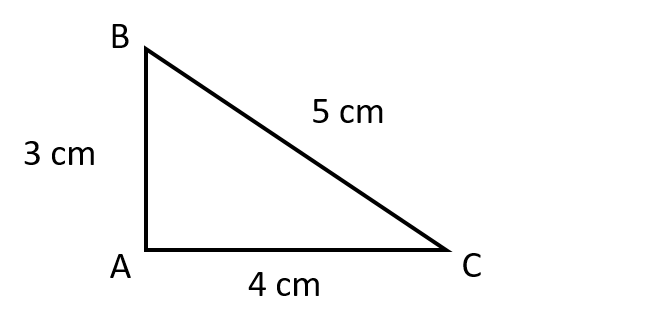
\includegraphics[scale=0.4]{Revision/Triangle_rectangle.png}
\end{figure}
\newpage
\textbf{2.} Le triangle ci-dessous est rectangle en A. Calculer la longueur AC :
\begin{figure}[!h]
    \centering
    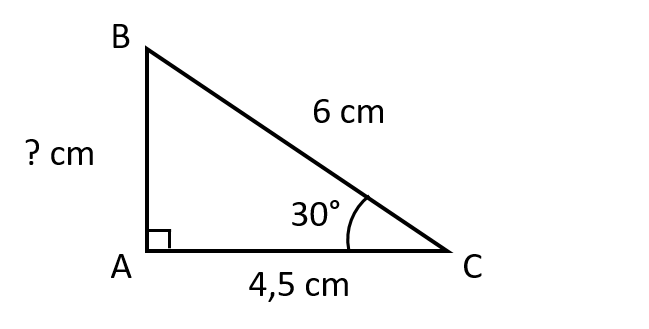
\includegraphics[scale=0.4]{Revision/Triangle_rectangle_2.png}
\end{figure}

\section{Physique}

\subsection{Record de vitesse ferroviaire}
Le projet de train japonais à sustentasion magnétique, le SCMaglev, a atteint la vitesse record de $603$~km/h en 2015. Ce train a la particularité de léviter au-dessus des rails. Pour rappel, un TGV roule à une vitesse de l'ordre de $300$~km/h en France.\\
\begin{enumerate}
    \item Convertir les deux vitesses en $m/s$.
    \item La distance entre Paris et Brest est de 500 km. En combien de temps une voiture roulant en moyenne à $100$~km/h effectue-t-elle ce trajet ? Et un TGV ? Et un SCMaglev ?
    \item Sachant que la distance Terre-Lune est de $380 000$~km, en combien de temps un SCMaglev peut-il atteindre la Lune ? On donnera la réponse en années/ jours/heures/minutes/secondes.
    \item A votre avis, quels sont les avantages du SCMaglev ?
\end{enumerate}

\subsection{Electricité}
\begin{enumerate}
    \item Avec quel instrument mesure-t-on une tension ? En quelle unité exprime-t-on le résultat ?
    \item Mêmes questions pour un courant.
    \item Une ampoule électrique est traversée par un courant I = $0,5$~A, et la tension à ses bornes est $U= 6$~V. Quelle est sa résistance ? Quelle puissance électrique $P$ consomme-t-elle ? 
    \item Faut-il utiliser un fil de cuivre ou un fil en caoutchouc pour conduire le courant ?
\end{enumerate}

\subsection{\'{E}nergie}
On rappelle qu’un corps de masse $m$ se déplaçant à la vitesse $v$ possède une énergie cinétique $E_c$ donnée par :
\begin{equation}
    E_c = \frac{1}{2}mv^2
\end{equation}
avec $E_c$ en J (Joule), $v$ en m/s et $m$ en kg.
\begin{enumerate}
    \item Une voiture pèse $m=1,2$ T. Convertir ce résultat en kg.
    \item Si cette voiture de masse roule à $50$~km/h, quelle est son énergie cinétique ?
    \item \textit{(bonus)} On branche pendant $\Delta t =1$~s une centrale nucléaire délivrant $1$~GW de puissance électrique à une voiture de masse $m=1000$~kg. \`{A} quelle vitesse va la voiture au bout de $\Delta t$ si on suppose que toutes l'énergie électrique fournit par la centrale a été convertie en énergie cinétique ?
\end{enumerate}

\section{Chimie}
\subsection{Atomes et petits pois}
\begin{enumerate}
    \item Quelle est la taille approximative d’un atome ? L’exprimer en m sous forme d’une puissance de 10.
    \item Combien d’atomes faut-il aligner pour obtenir une chaîne de longueur 1 mm ?
    \item Quels sont les principaux constituants d’un atome ?
    \item Modéliser physiquement un petit pois (forme, taille, ...). Si le noyau d’un atome avait la taille d’un petit pois, quelle taille aurait l’atome entier ?
\end{enumerate} 

\subsection{Verrerie}
\textbf{1.} Nommer la verrerie présentée ci-dessous :
\begin{figure}[!h]
    \centering
    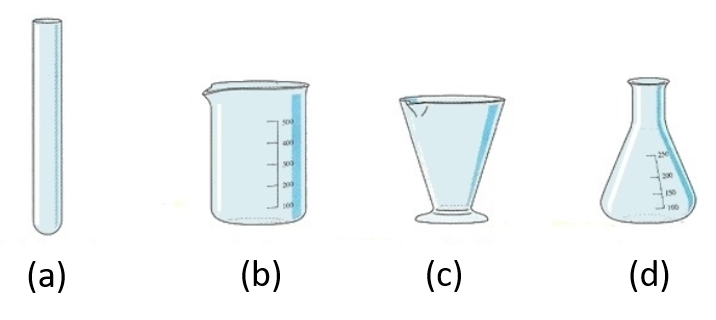
\includegraphics[scale=0.4]{Revision/Verrerie1.png}
\end{figure}

\textbf{2.} Proposer deux méthodes pour peser une masse $m=10$~g d'eau. On rappelle que la masse volumique de l'eau vaut $\rho=1$~g.mL${-1}$.
  %%\newpage
%$ $
%\newpage

\renewcommand{\thesubsection}{\textcolor{red}{\Roman{section}.\arabic{subsection}}}
\renewcommand{\thesubsubsection}{\textcolor{red}{\Roman{section}.\arabic{subsection}.\alph{subsubsection}}}

\setcounter{section}{0}
\sndEnTeteTPO

\begin{center}
\begin{mdframed}[style=titr, leftmargin=60pt, rightmargin=60pt, innertopmargin=7pt, innerbottommargin=7pt, innerrightmargin=8pt, innerleftmargin=8pt]

\begin{center}
\large{\textbf{TP 0: Des mesures en tout sens}}
\end{center}

\end{mdframed}
\end{center}



\begin{tcolorbox}[colback=blue!5!white,colframe=blue!75!black,title=Objectifs de la séance :]
\begin{itemize}
    \item S'approprier du matériel de mesure
    \item Appréhender les incertitudes d'une mesure
    \item Travailler en groupe
\end{itemize}
\end{tcolorbox}

Pour cette première séance de TP de l'année, nous allons manipuler quelques outils de mesures pour comprendre les sources d'incertitudes associées à ces mesures.

\section{Mesure du temps}
\begin{mdframed}[style=autreexo]
\textbf{\bsc{Liste du matériel}}
\begin{itemize}
    \item un pendule pesant
    \item un chronomètre
\end{itemize}
\end{mdframed}
\begin{Large}{\textbf{Q :}} \end{Large} La période d'oscillation d'un pendule est définie comme le temps au bout duquel le pendule a fait un aller-retour. Selon vous, comment peut-on mesurer le plus précisément la période d'oscillation du pendule ? \\
\newline
\newline
\underline{$1^{\text{ère}}$ méthode :} Lâcher le pendule d'une faible hauteur. Chaque élève mesure une période d'oscillation. \textbf{Comparer vos mesures entre vous et Commenter }:
\vspace{8cm}

\underline{$2^{\text{ème}}$ méthode :} Chaque binôme mesure 5 fois une période de manière indépendante. Notez les valeurs obtenues par binôme dans le tableau suivant :
\\

\begin{tabular}{|l|C{0.14}|C{0.14}|C{0.14}|C{0.14}|C{0.14}|C{0.14}|C{0.14}|C{0.14}|C{0.14}|C{0.14}|}
\hline
     Mesure n$^{\circ}$ & 1 & 2 & 3 & 4 & 5 \\
     \hline
     Période (en s) & & & & & \\
     \hline
\end{tabular}
\newline
\newline

\begin{tcolorbox}[colback=blue!5!white,colframe=white!75!black,title=Document 1 :]
La moyenne d'une mesure est la somme de toutes les valeurs mesurées divisée par le nombre de mesures effectuées :
\begin{equation*}
    \text{Moyenne} = \frac{\text{Mesure n$^{\circ}$1}+\text{Mesure n$^{\circ}$2} + ... + \text{Mesure n$^{\circ}$N}}{\text{N}}
\end{equation*}
L'écart-type représente la dispersion (c'est-à-dire à quel point les mesures changent d'une mesure à une autre) associée à une série d'une mesure. Elle est donnée par :
\begin{equation*}
    \text{Ecart-type }= \sqrt{\frac{\left(\text{Mesure n$^{\circ}$1}-\text{Moyenne}\right)^2+...+\left(\text{Mesure n$^{\circ}$N}-\text{Moyenne}\right)^2}{\text{N}}}
\end{equation*}
\end{tcolorbox}

\begin{tcolorbox}[colback=blue!5!white,colframe=white!75!black,title=Document 2 :]
On représente le résultat d'une mesure selon la manière suivante :
\begin{equation*}
    \text{Résultat} = \text{Moyenne} \pm \text{incertitude-type}
\end{equation*}
\end{tcolorbox}
\textbf{Travail à faire :} Calculer la moyenne notée $<T>$ de la période d'oscillation du pendule et évaluer qualitativement son incertitude-type. \underline{Pour les plus rapides :} calculer l'écart-type de vos mesures.

\newpage

\section{Mesure de la masse d'une bille de plomb}

\begin{mdframed}[style=autreexo]
\textbf{\bsc{Liste du matériel}}
\begin{itemize}
    \item 1 pied à coulisse
    \item 1 règle
    \item 1 balance
\end{itemize}
\end{mdframed}

\begin{tcolorbox}[colback=blue!5!white,colframe=white!75!black,title=Document 3 :]La masse $m$ d'une bille de plomb est reliée à son rayon $R$ et à sa masse volumique $\rho$ par la formule suivante :
\begin{equation*}
    m = \frac{4\pi R^3\times\rho}{3}
\end{equation*}
\end{tcolorbox}

\begin{Large}{\textbf{Q :}} \end{Large} Choisissez une bille de plomb, comment mesurer sa masse ? On donne $\rho=$
\newline
\newline

\underline{$1^{\text{ère}}$ méthode :} Mesurer la masse à la balance. \textbf{Commenter :}
\vspace{5cm}

\underline{$1^{\text{ère}}$ méthode :} Mesurer le rayon de la bille. En déduire la masse à l'aide du Document 3. \textbf{Commenter :}


\newpage

\section*{Conclusion du TP}

\begin{tcolorbox}[colback=red!5!white,colframe=red!75!black,title=\textbf{On retiendra : }]
\begin{enumerate}
    \item L'instrument de mesure et le protocole expérimental influent sur le résultat d'une mesure,
    \item On écrit un résultat expérimental final en prenant en compte son incertitude :
    \begin{equation*}
        \text{Résultat} = \text{Moyenne} \pm \text{incertitude-type}
    \end{equation*}
    \item On peut améliorer la mesure d'une grandeur physique en la répétant plusieurs fois et en calculant sa moyenne,
    \item On écrit un résultat en adaptant le nombre de chiffres significatifs.
\end{enumerate}
\end{tcolorbox}


%% Devoir Commun de seconde
   %\modeCorrection

%%%% Définition En-tête et pied de page 
\pagestyle{fancy}
\renewcommand\footrulewidth{1pt}
\fancyhead[L]{Devoir commun de Physique-Chimie}
\fancyhead[R]{Lycée Parc de Vilgénis}
\fancyfoot[C]{\textbf{Page \thepage/\pageref{LastPage}}}

\renewcommand{\thesubsection}{\textcolor{red}{\Roman{section}.\arabic{subsection}}}
\renewcommand{\thesubsubsection}{\textcolor{red}{\Roman{section}.\arabic{subsection}.\alph{subsubsection}}}
\renewcommand{\titreDocu}[1]{
  \refstepcounter{document} % update counter
  \textbf{Exercice \arabic{document} -- #1} 
  \addcontentsline{toc}{document}{\protect\numberline{} #1} % update table of content
}


\renewcommand{\numeroQuestion}{
  \refstepcounter{exercice}
  \vspace*{2pt}
  \hspace{15pt}
  \textcolor{black}{%couleurPrincipale!75!black}{
    \textbf{Q.\arabic{exercice}}
  }
}

\setcounter{section}{0}
\setcounter{document}{0}


%\nomPrenomClasse
\vspace{1cm}

\begin{center}
\begin{Huge}
    DEVOIR COMMUN DE SECONDE
\end{Huge}
\end{center}
\vspace{1cm}

\vspace{1cm}

\begin{center}
    \begin{large}
        Jeudi 21 Décembre 2023
    \end{large}
\end{center}

\vspace{2cm}

\begin{center}
    \begin{Large}
        \textbf{PHYSIQUE-CHIMIE}\\
    \end{Large}
\end{center}
\vspace{2cm}


\begin{center}
    \begin{large}
        Durée de l'épreuve : \textbf{2 heures}\\
    \end{large}
\end{center}
\vspace{1cm}
\begin{center}
    \begin{large}
        \textit{L'usage de la calculatrice est autorisé.}\\
    \end{large}
\end{center}
\vspace{1cm}
\begin{center}
    \begin{large}
        Dès que ce sujet vous est remis, assurez-vous qu’il est complet.\\
        Ce sujet comporte \pageref{LastPage} pages numérotées de \thepage/\pageref{LastPage} à \pageref{LastPage}/\pageref{LastPage}.
    \end{large}
\end{center}

\begin{tcolorbox}[colback=red!5!white,colframe=red!75!black,title=\textbf{Consignes : }]
   \begin{enumerate}
       \item Pour les élèves bénéficiant d'un tiers-temps, vous ne traiterez pas les questions marquées par $(*)$ ; 
       \item Lisez-bien l'énoncé des exercices. Les questions sont pour la plupart indépendantes. Si vous bloquez sur une question, passez à la suivante ;
       \item N'oubliez pas d'encadrer ou de souligner vos résultats ;
       \item Vous rendrez l'énoncé avec la copie.
   \end{enumerate}
\end{tcolorbox}
\newpage

%\begin{tableauCompetences}
%    APP & S'approprier les informations d'un document & & & & \\
%    \hline
%    REA & Utiliser les pourcentages et les fractions  & & & & \\
%     \hline 
%    ANA &  Exploiter les informations extraites des données & & & & \\
%    \hline
%    VAL & Valider/critiquer un modèle & & & &
%\end{tableauCompetences}



\begin{doc}{Le gaz de ville \begin{large}
    /9 points
\end{large}}
\vspace{-0.4cm}
\begin{wrapfigure}{r}{0.35\textwidth}
\vspace{-0cm}
    \centering
      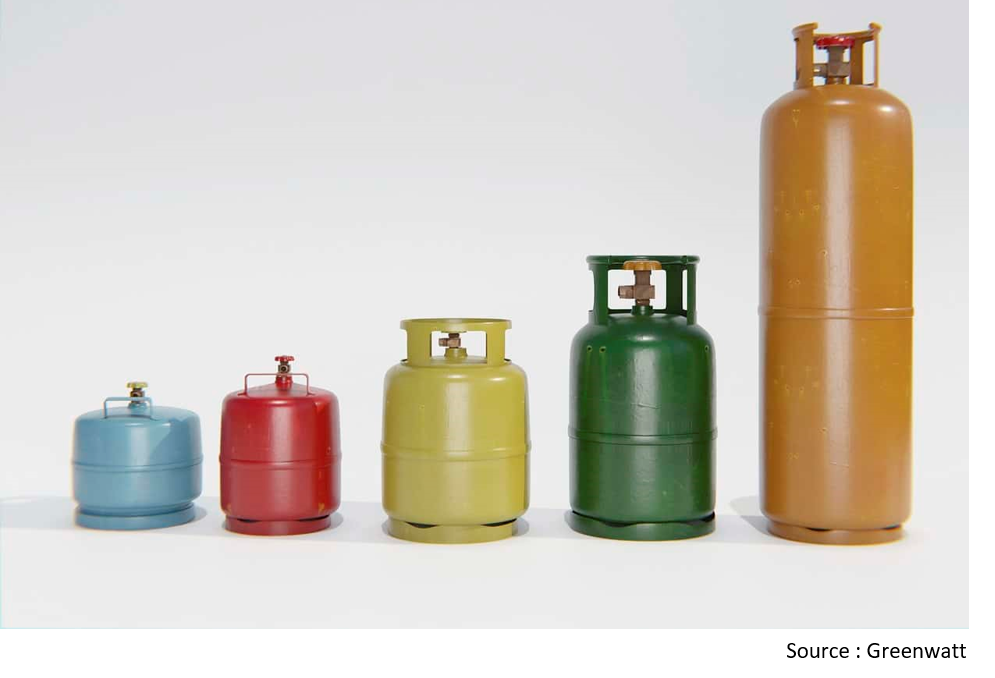
\includegraphics[scale=0.35]{Images/DS/Devoir_Commun/Bouteille_gaz.png}
  \end{wrapfigure}
L'odeur de gaz vous est désagréable, mais c'est pour votre bien ! Le saviez-vous ?\\
Le gaz de ville, celui qui arrive dans les habitations par des tuyaux de distribution collective, est principalement constitué de méthane. Le méthane est incolore et inodore, mais alors d'où vient l'odeur si caractéristique du gaz de ville ?\\
Ce que l'on appelle « odeur de gaz » est en réalité dû à un additif ajouté, le tétrahydrothiophène (THT), pour rendre les fuites de gaz détectables et prévenir du danger qu’elles représentent. En effet, le méthane devient fortement explosif lorsqu'il atteint une certaine concentration dans l'air.\\

On considère une bouteille de gaz de ville de volume $V=100$~L. L’étiquette sur la bouteille indique le pourcentage volumique des deux espèces chimiques présentes dans ce mélange :

\begin{center}
    \begin{tabular}{|C{0.45}|C{0.45}|}
        \hline
        \multicolumn{2}{|c|}{\cellcolor{blue!25}Composition du mélange contenu dans la bouteille de gaz de ville} \\
        \hline
        \cellcolor{orange!25}Nom de la substance & \cellcolor{orange!25}Pourcentage volumique \\
        \hline
        tétrahydrothiophène (THT) & 0,10225 \% \\
        \hline 
         Méthane & 99,89775 \%  \\
         \hline
    \end{tabular}
\end{center}
Voici quelques données sur le méthane :
\begin{center}
    \begin{tabular}{|c|C{0.3}|}
        \hline
        \cellcolor{orange!25}Pictogrammes de sécurité du méthane &
            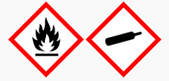
\includegraphics[scale=0.3]{Images/DS/Devoir_Commun/Picto.png}
         \\
        \hline
        \cellcolor{orange!25}Température de fusion (en $\degreCelsius$) à la pression atmosphérique & $-182,47$ \\
        \hline
        \cellcolor{orange!25}Température d'ébullition (en $\degreCelsius$) à la pression atmosphérique & $-161,52$ \\
        \hline 
        \cellcolor{orange!25}Masse volumique du méthane (en g$\cdot$L$^{-1}$) & 0,657 \\
         \hline
    \end{tabular}
\end{center}


\question{Rappeler la définition d’un mélange et proposer un exemple. (1pt)}{~}{0}
%\\
\vspace{-0.2cm}
\question{Il est conseillé de ne pas conserver une bouteille de méthane à proximité d’une fenêtre exposée au soleil. Justifier à l’aide des pictogrammes de sécurité du méthane.(1pt)
}{}{0}
%\\
\vspace{-0.2cm}
\question{Indiquer l’état physique du méthane à température ambiante (20°C) et à la pression atmosphérique. Justifier. (1pt)}{}{0}
%\\
\vspace{-0.2cm}
\question{\`{A} l’aide des documents, déterminer le volume de chaque espèce chimique présente dans la bouteille de gaz de ville. (2pts)}{~}{0}
\newpage%\\
\question{$(*)$ En déduire la masse de méthane $m_{\text{méthane}}$ contenue dans la bouteille. (1pt)}{~}{0}
%\\
Voici un graphe donnant la masse volumique du mélange méthane/THT en fonction du pourcentage volumique du THT dans le mélange : 
\begin{center}
    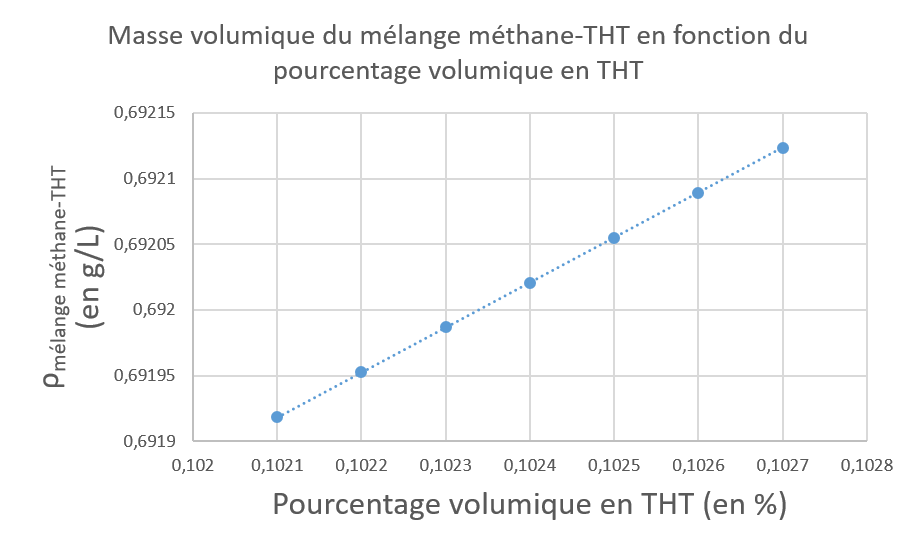
\includegraphics[scale=1]{Images/DS/Devoir_Commun/Graphe_rhovspourcentagevol.png}
\end{center}
\question{Déterminer graphiquement la masse volumique du mélange $\rho_{\text{mélange}}$ dans la bouteille de gaz de ville. Vous ferez apparaître la construction sur le graphique. (1pt)}{~}{0}
%\\
\textbf{Pour la question suivante, toute tentative de réponse même non aboutie sera valorisée.}\\
\question{$(*)$ La norme imposée au gaz de ville est qu’il doit contenir entre $15$~mg et $40$~mg de THT par litre de gaz. Exprimer la masse volumique du mélange en fonction de la masse des espèces chimiques et du volume de la bouteille. En déduire la masse de THT présente dans la bouteille de gaz étudiée. Respecte-t-elle la norme imposée au gaz de ville ? Justifier en rédigeant une réponse scientifiquement argumentée. (2pts)}{On trouve 36~mg.}{0}
%\\
\end{doc}

%%%%%%%%%%%%%%%%%%%%%%%%%%%%%%%%%
\newpage
%%%%%%%%%%%%%%%%%%%%%%%%%%%%%%%%%
\setcounter{exercice}{0}
\begin{doc}{Solutions aqueuses \begin{Large}
    /9 points
\end{Large}}
\begin{wrapfigure}{r}{0.3\textwidth}
\vspace{-1cm}
    \centering
      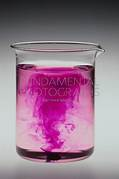
\includegraphics[scale=1.0]{Images/DS/Devoir_Commun/Permanganate.png}
  \end{wrapfigure}
\og Le permanganate de potassium est un solide gris-violet de formule \chemform{KMnO_4}. Dissous dans l’eau, il donne des solutions de couleur violette.\\
Pour soigner les érythèmes (irritations de la peau), il est recommandé d’utiliser des solutions aqueuses de permanganate de potassium de concentration en masse égale à $0,10$~g$\cdot$L$^{-1}$.\\
En solution aqueuse à $0,50$~g$\cdot$L$^{-1}$, le permanganate de potassium est également utilisé comme désinfectant pour laver les légumes dans les pays tropicaux.\fg
\begin{flushright}
    \textit{D’après le site \url{ societechimiquedefrance.fr/permanganate-de-potassium}}.
\end{flushright}

L’objectif de l’exercice est d’estimer la concentration d’une solution aqueuse S de permanganate de potassium afin de valider ou non son utilisation pour soigner les érythèmes ou pour laver les légumes.\\

Pour cela, on prépare 250 mL d’une solution aqueuse S$_0$ de permanganate de potassium de concentration en masse $C_{m,0} = 0,60$~g$\cdot$L$^{-1}$ en dissolvant dans l’eau une masse appropriée de permanganate de potassium solide.\\


\question{Identifier le solvant et le soluté des solutions utilisées pour soigner les érythèmes ou pour laver les légumes. (1pt)}{Solvant : eau, soluté : \chemform{KMnO_4}.}{0}
%\\
\question{$(*)$ Donner le nom de la technique utilisée pour préparer la solution S$_0$. (0,5pt)}{Il s'agit d'une dissolution.}{0}
%\\
\question{Donner l’expression de la concentration en masse $C_m$ d’une solution en fonction de la masse de soluté $m_{\text{soluté}}$ et du volume de solution $V_{\text{solution}}$. (0,5pt)}{}{0}
%\\
\question{En déduire la valeur de la masse de permanganate de potassium qui a été dissoute pour préparer 250 mL de solution S$_0$. (1,5pts)}{~}{0}
%\\

\newpage
On prépare ensuite cinq solutions S$_1$, S$_2$, S$_3$, S$_4$ et S$_5$ en prélevant différents volumes de solution aqueuse S$_0$ de permanganate de potassium de concentration en masse $C_{m,0} = 0,60$~g$\cdot$L$^{-1}$ et en y ajoutant de l’eau distillée pour obtenir un volume de 50,0 mL de solution (voir tableau ci-après).
\begin{center}
    \begin{tabular}{|C{0.1}|C{0.2}|C{0.2}|C{0.3}|}
        \hline
        \cellcolor{blue!25}Solution & \cellcolor{blue!25}Volume de solution S$_0$ à prélever (mL) & \cellcolor{blue!25}Volume de solution obtenue (mL) & \cellcolor{blue!25}Concentration en masse de la solution obtenue (g$\cdot$L$^{-1}$) \\
        \hline 
        S$_1$ & 2 & 50,0 & 0,024 \\
        \hline
        S$_2$ & 5 & 50,0 & 0,060 \\
        \hline
        S$_3$ & 10 & 50,0 & 0,12 \\
        \hline
        S$_4$ & 15 & 50,0 & 0,18 \\
        \hline
        S$_5$ & ~? & 50,0 & 0,24 \\
        \hline
    \end{tabular}
\end{center}

\question{Donner le nom de la technique utilisée pour préparer les cinq solutions S$_1$, S$_2$, S$_3$, S$_4$ et S$_5$. (0,5pt)}{Il s'agit d'une dilution.}{0}
%\\
\question{Écrire le protocole expérimental qui a été suivi pour préparer 50,0 mL de solution S$_1$. Préciser soigneusement le nom du matériel utilisé. (1,5pts)}{~}{0}
%\\
\question{Déterminer la valeur du volume de solution S$_0$ qui a été prélevé pour préparer 50,0 mL de solution S$_5$. Justifier précisément le calcul effectué. (2pts)}{~}{0}
%\\
On verse les cinq solutions S$_1$, S$_2$, S$_3$, S$_4$ et S$_5$ dans des tubes à essais : on obtient ainsi une échelle de teintes (voir photo ci-dessous).
\begin{center}
    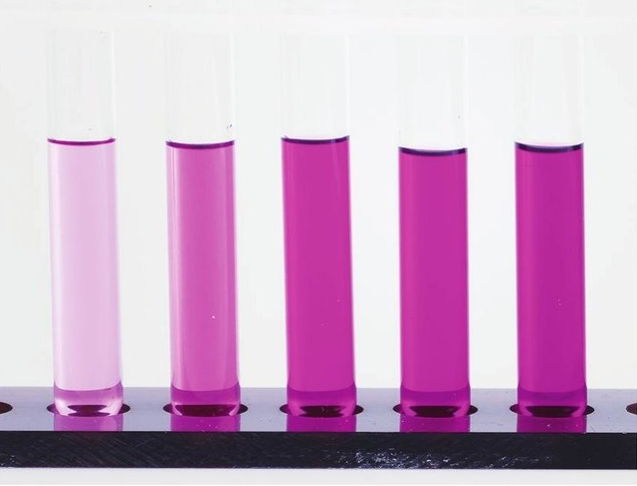
\includegraphics[scale=0.5]{Images/DS/Devoir_Commun/Echelle_teinte.png}
\end{center}
On verse ensuite la solution S dans un sixième tube à essais. On constate que la teinte de la solution S est comprise entre celles des solutions S$_2$ et S$_3$.\\
\question{Déterminer un encadrement de la concentration en masse de la solution S. (1pt)}{$0,060~\text{g$\cdot$L$^{-1}$}<C_{m,0}<0,12~\text{g$\cdot$L$^{-1}$}$}{0}
%\\
\question{$(*)$ En déduire si la solution $S$ peut être utilisée pour soigner les érythèmes ou pour laver les légumes. Justifier.(0,5pt)}{~}{0}
\end{doc}
\setcounter{exercice}{0}
\begin{doc}{Le son d’une guitare
 \begin{Large}
    /12 points
\end{Large}}
Une guitare se compose d'un coffre auquel est accroché un manche sur lequel sont tendues des cordes métalliques ou en nylon. La photo ci-dessous présente une guitare ainsi qu'un zoom sur une partie du manche après avoir frotté les cordes :

\begin{center}
    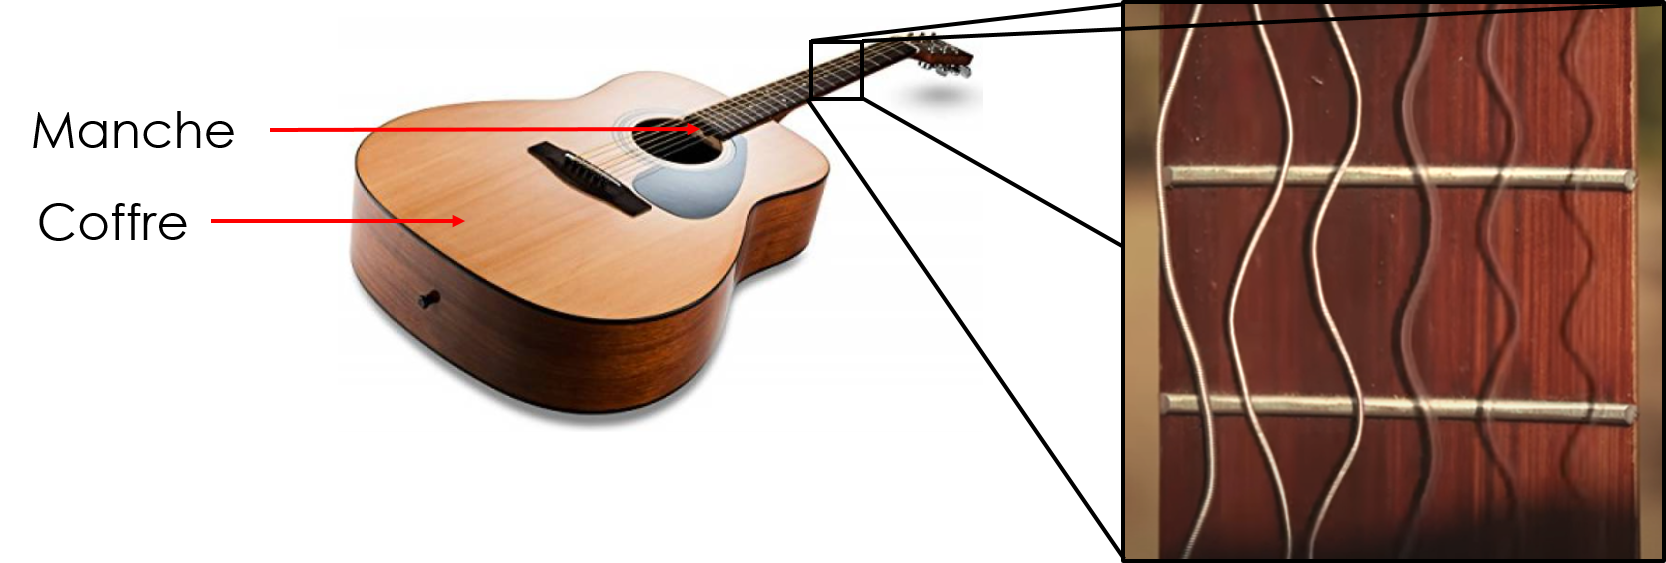
\includegraphics[scale=0.5]{Images/DS/Devoir_Commun/Guitare.png}
\end{center}

Voici un tableau des notes (do, ré, mi, fa, sol, la, si) et des fréquences (en Hz) correspondantes de la gamme tempérée :
\begin{center}
    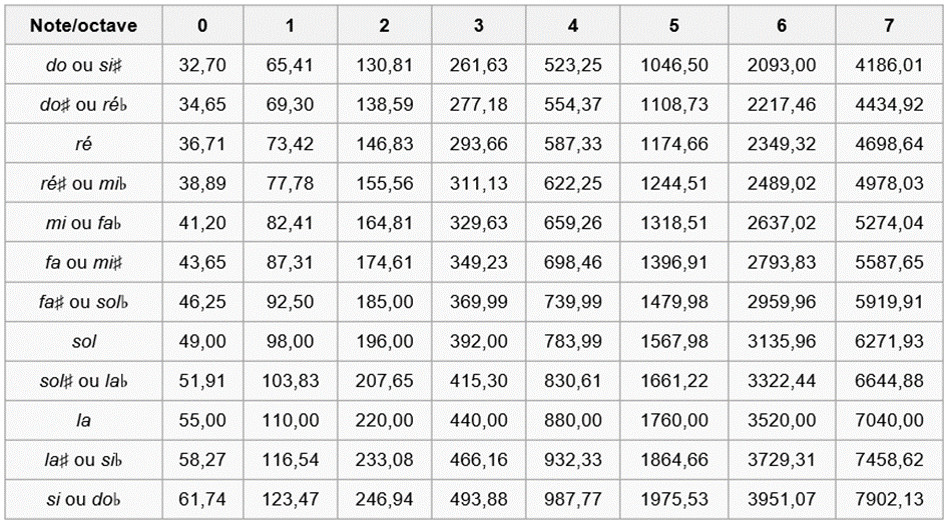
\includegraphics[scale=0.7]{Images/DS/Devoir_Commun/Notes_guitare.png}
\end{center}

On dit qu'une note est jouée \og à vide \fg~ lorsqu'on laisse la corde de guitare vibrer librement sur toute sa longueur. De la corde la plus épaisse à la plus fine, les six notes jouées à vide sont : \og mi2, la2, ré3, sol3, si3, mi4 \fg~.
\newpage
\question{Indiquer l'origine du son émis par une guitare. (1pt)}{Les cordes vibrent et font vibrer les molécules d'air de proche en proche.}{0}
%\\
\question{Donner l'intérêt physique du coffre d'une guitare. (1pt)}{Le coffre sert de caisse de résonance, c'est-à-dire qu'il sélectionne et amplifie et le son émis par le frottement des cordes de guitare.}{0}
%\\
\question{Indiquer la condition pour que le son se propage dans un milieu. (0,5pt)}{Il faut un milieu matériel pour que le son puisse se propager}{0}
%\\
\question{Identifier le milieu dans lequel le son se propage de la guitare jusqu'à notre oreille puis rappeler la valeur de la vitesse de propagation du son dans ce milieu. (1pt)}{Ici, le milieu est l'air et la vitesse vaut (à $15\degreCelsius$) 340~m$\cdot$s$^{-1}$.}{0}
%\\
\question{Calculer la durée $\Delta t$ que met le son à se propager jusqu’à l’auditeur lorsqu'il se trouve à une distance d=1km. (2pts). \textit{(Bonus) : l'auditeur parviendre-t'il a entendre ce son ? Justifier. (1pt)}}{~}{0}
%\\
\question{$(*)$ Donner le domaine des fréquences audibles pour un être humain. (1pt)}{Entre 20~Hz et 20000~Hz.}{0}
%\\
\question{Un chat est capable d’entendre des fréquences comprises entre 20 Hz et 60 kHz. Peut-il entendre la note la plus grave jouée avec une guitare ? Justifier la réponse. (1pt)}{Oui car la note la plus grave sonne à la fréquence 32,70~Hz qui est comprise dans le domaine de fréquence audible du chat.}{0}
%\\
\question{$(*)$ Donner les valeurs des fréquences des 6 notes jouées à vides à la guitare. (1,5pts)}{~}{0}
%\\
\question{Entre la note mi2 et la note mi3, donner le son le plus aigu. Justifier.(1pt)}{~}{0}
%\\
Un ingénieur du son a enregistré une note émise par une guitare, à l’aide d’un microphone relié à un système informatisé. Voici le signal enregistré :
\begin{center}
    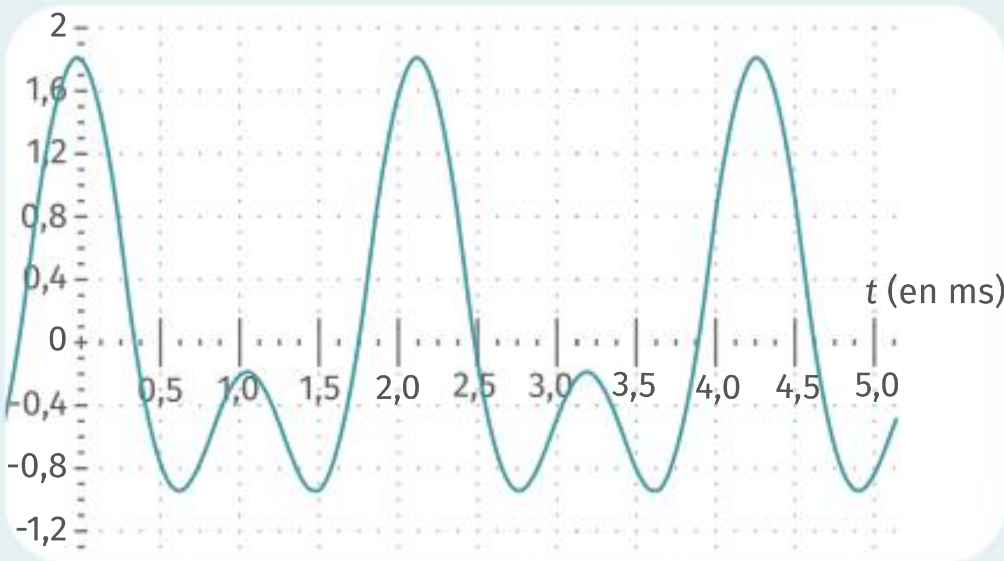
\includegraphics[scale=0.5]{Images/DS/Devoir_Commun/Signal_guitare.PNG}
\end{center}
\question{Donner la formule reliant la fréquence $f$ et la période $T$ d’un signal. Déterminer la fréquence $f$ de la note émise par la guitare. (2pts)}{~}{0}

\end{doc}
\vspace{2cm}
\begin{center}
\begin{Huge}
    \textbf{FIN DU SUJET.}
\end{Huge}
\end{center}
  
%% Chapitre 1 : Corps purs et mélange au quotidien
  %%\newpage
%$ $
%\newpage

\renewcommand{\thesubsection}{\textcolor{red}{\Roman{section}.\arabic{subsection}}}
\renewcommand{\thesubsubsection}{\textcolor{red}{\Roman{section}.\arabic{subsection}.\alph{subsubsection}}}

\setcounter{section}{0}
\sndEnTeteDeux

\begin{center}
\begin{mdframed}[style=titr, leftmargin=60pt, rightmargin=60pt, innertopmargin=7pt, innerbottommargin=7pt, innerrightmargin=8pt, innerleftmargin=8pt]

\begin{center}
\large{\textbf{Chapitre 1: Corps purs et mélanges au quotidien}}
\end{center}

\end{mdframed}
\end{center}
Ce chapitre permet de faire une description de la matière à l'échelle macroscopique (c'est-à-dire à notre échelle). Posons-nous les questions suivantes : Qu'est-ce qu'une espèce chimique ? Comment faire pour en identifier une en laboratoire ? Comment reconnaître un mélange d'une espèce chimique unique ?
%
\begin{tcolorbox}[colback=blue!5!white,colframe=blue!75!black,title=Mots clés du chapitre :]
Corps purs, mélange homogène/hétérogène, masse volumique, températures de changement d'état, solubilité.
\end{tcolorbox}

%

\section{Définitions}

\subsection{Espèces chimiques}

La matière est constituée d'\textcolor{red}{entités chimiques} : les atomes, les molécules, les ions. \`{A} partir de ces entités, on peut définir une \textcolor{red}{espèce chimique} :
\begin{tcolorbox}[colback=green!5!white,colframe=green!75!black,title=\textbf{Espèce chimique}, upperbox=invisible]
Elle est composée d'un ensemble d'entités chimiques identiques. Une espèce chimique est caractérisée par :
\begin{itemize}
    \item sa formule chimique : par exemple \chemform{H_2O} pour l'eau,
    \item son aspect : couleur, texture, forme, ...
    \item ses propriétés physiques : température d'ébullition, masse volumique, indice de réfraction, ...
    \item ses propriétés chimiques : réactivité avec d'autres espèces chimiques, ... 
    \item 
    \item
\end{itemize}

\end{tcolorbox}

\begin{mdframed}[style=autreexo]
\textbf{\bsc{Exercice de cours 1} - Espèces chimiques}\\
Donner le type (\textit{atomique}, \textit{moléculaire} ou \textit{ionique}) des espèces chimiques suivantes : hélium (He), eau (H\textsubscript{2}O), chlorure de sodium (Na$^{+}$, Cl$^{-}$).
\end{mdframed}

On distingue alors les \textcolor{red}{corps purs} et les \textcolor{red}{mélanges}.

\subsection{Les corps purs}
\begin{tcolorbox}[colback=green!5!white,colframe=green!75!black,title=\textbf{Corps purs}]
Un corps pur est constitué d'une\gap{...............} espèce chimique.
\end{tcolorbox}

Les corps purs peuvent être :

\begin{itemize}
    \item \textcolor{red}{simples} : ils sont constitués d'un seul type d'atome. Exemples : le dihydrogène \chemform{H_2}, le charbon \chemform{C}, l'argent \chemform{Ag}.
    \item \textcolor{red}{composés} : ils sont constitués de plusieurs atomes dans des proportions bien définies. Exemples : l'eau \chemform{H_2O}, l'éthanol \chemform{C_2H_6O}, le chlorure de sodium \chemform{(Na^+;Cl^-)}.
\end{itemize}

%%%%%%%%



%
\subsection{Le cas des mélanges}
\begin{tcolorbox}[colback=green!5!white,colframe=green!75!black,title=\textbf{Mélange}]
Un mélange est constitué de \gap{...............} espèces chimiques différentes.
\end{tcolorbox}
Les mélanges peuvent être :
\begin{itemize}
    \item \textcolor{red}{homogènes} : ils sont constitués d'une seule phase (solide, liquide ou vapeur) indiscernable à l'\oe il nu. Lorsque deux liquides se mélangent l'un avec l'autre, on dit qu'ils sont \textcolor{red}{miscibles}.
    \item \textcolor{red}{hétérogènes} : ils sont constitués de plusieurs phases discernables à l'\oe il nu.
\end{itemize}

\begin{mdframed}[style=autreexo]
\textbf{\bsc{Exercice de cours 2} - Corps purs et mélanges}\\
Pour chaque substance suivante, dire s’il s’agit d’un corps pur simple/complexe ou d’un mélange homogène/hétérogène.
\end{mdframed}
\begin{table*}
    \centering
    \begin{tabular}{|C{0.15}|C{0.15}|c|c|C{0.15}|}
    \hline
    Description & Bécher d'huile et d'eau & Bécher d'huile & Bécher d'eau pure & Bécher d'azote liquide \\
    \hline
    Photographie & 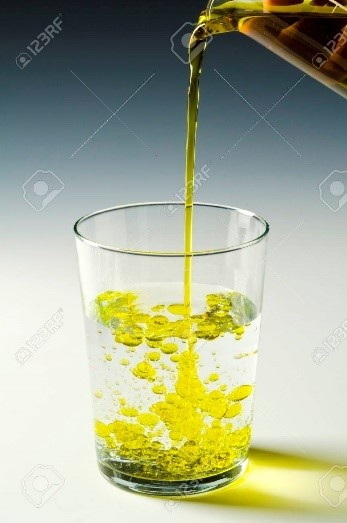
\includegraphics[scale=0.6]{Images/Chapitre_1/Becher_huile_eau.jpg} & 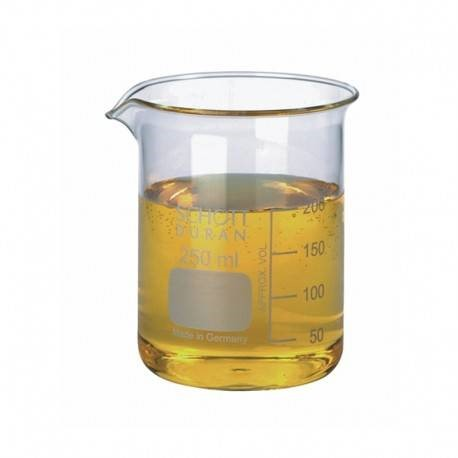
\includegraphics[scale=0.3]{Images/Chapitre_1/Becher_huile.jpg} & 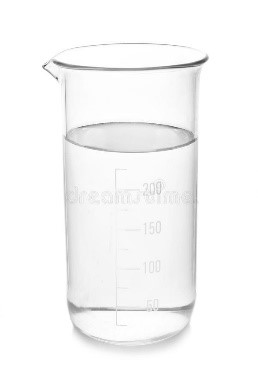
\includegraphics[scale=0.7]{Images/Chapitre_1/Becher_eau.jpg} & 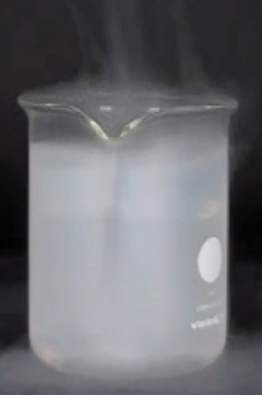
\includegraphics[scale=0.3]{Images/Chapitre_1/Becher_azote.png} \\
    \hline
    Type de corps & & & & \\
    \hline
    Qualificatif du corps & & & & \\
    \hline
   \end{tabular}
\end{table*}

\section{Identification d'espèces chimiques}
Comment reconnaitre expérimentalement une espèce chimique par rapport à une autre ? On présente dans cette partie quelques éléments qui vont nous permettre de répondre à cette question.

\subsection{Tests chimiques}
\begin{tcolorbox}[colback=red!5!white,colframe=red!75!black,title=\textbf{Tests chimiques à connaître : }]
%\begin{table}
    %\centering
   \begin{tabular}{|C{0.31}|C{0.3}|C{0.31}|}
   \hline
    \cellcolor{blue!25} Espèce chimique à tester & \cellcolor{blue!25} Test & \cellcolor{blue!25} Résultat du test positif \\
    \hline
    Eau (\chemform{H_2O}) & Sulfate de cuivre anhydre (solide blanc)  &  \\
    \hline
    Dioxygène (\chemform{O_2}) & Bûche incandescente &  \\
    \hline
    Dihydrogène (\chemform{H_2}) & Allumette enflammée  &  \\
    \hline 
    Dioxyde de carbone (\chemform{CO_2}) & Eaux de chaux & \\
    \hline
    \end{tabular}
%\end{table}
\end{tcolorbox} 

\subsection{Propriétés physiques}
\subsubsection{La masse volumique}
\begin{tcolorbox}[colback=green!5!white,colframe=green!75!black,title=\textbf{Rappel : masse volumique et densité }]
La masse volumique d'une espèce chimique est :
\begin{equation*}
    \rho = \frac{m}{V}
\end{equation*}
avec m la masse de l'espèce et V son volume. Elle s'exprime en g.cm$^{-3}$.\\
La densité $d$ d'une espèce chimique est le rapport entre la masse volumique de cette substance et la masse volumique de l'eau liquide valant $\rho_{eau}=1$~g.cm$^{-3}$ :
\begin{equation*}
%    d = \frac{\rho_{espece}}{\rho_{eau}}
\end{equation*}
\importantbox{$d$ s'exprime sans unité puisqu'il s'agit d'un rapport entre deux grandeurs physique de même nature.}
\end{tcolorbox}

\begin{tcolorbox}[colback=red!5!white,colframe=red!75!black,title=\textbf{Masse volumique de l'eau: }]
\begin{center}
    $\rho_{eau} = $\gap{................}~kg.m$^{-3}$ ou \gap{.....}~g.cm$^{-3}$. 
\end{center}
\end{tcolorbox}

\begin{tabular}{|c|C{0.06}|C{0.06}|C{0.06}|C{0.1}|C{0.15}|C{0.1}|C{0.1}|}
   \hline
     & Vide & Air & Eau & Glace & Cyclohexane & Bronze & Or \\
    \hline
    $\rho$ (en g.cm$^{-3}$) & 0 & 0,001 & 1,0 & 0,92 & & 7,9 & 19  \\
    \hline
    d & 0 &  & 1 &  &  & & \\
    \hline
    \end{tabular}
\begin{mdframed}[style=autreexo]
\textbf{\bsc{Exercice de cours 3} - Masse volumique du cyclohexane}\\
\textbf{1)} Calculer la masse volumique du cyclohexane sachant qu'un volume de 15~mL a une masse de 11,8~g.\newline \textbf{2)} Le cyclohexane est-il plus dense que l'eau ? \end{mdframed}
\newpage

\subsubsection{Les températures de changement d'état}
\begin{figure}[!htb]
    \centering
    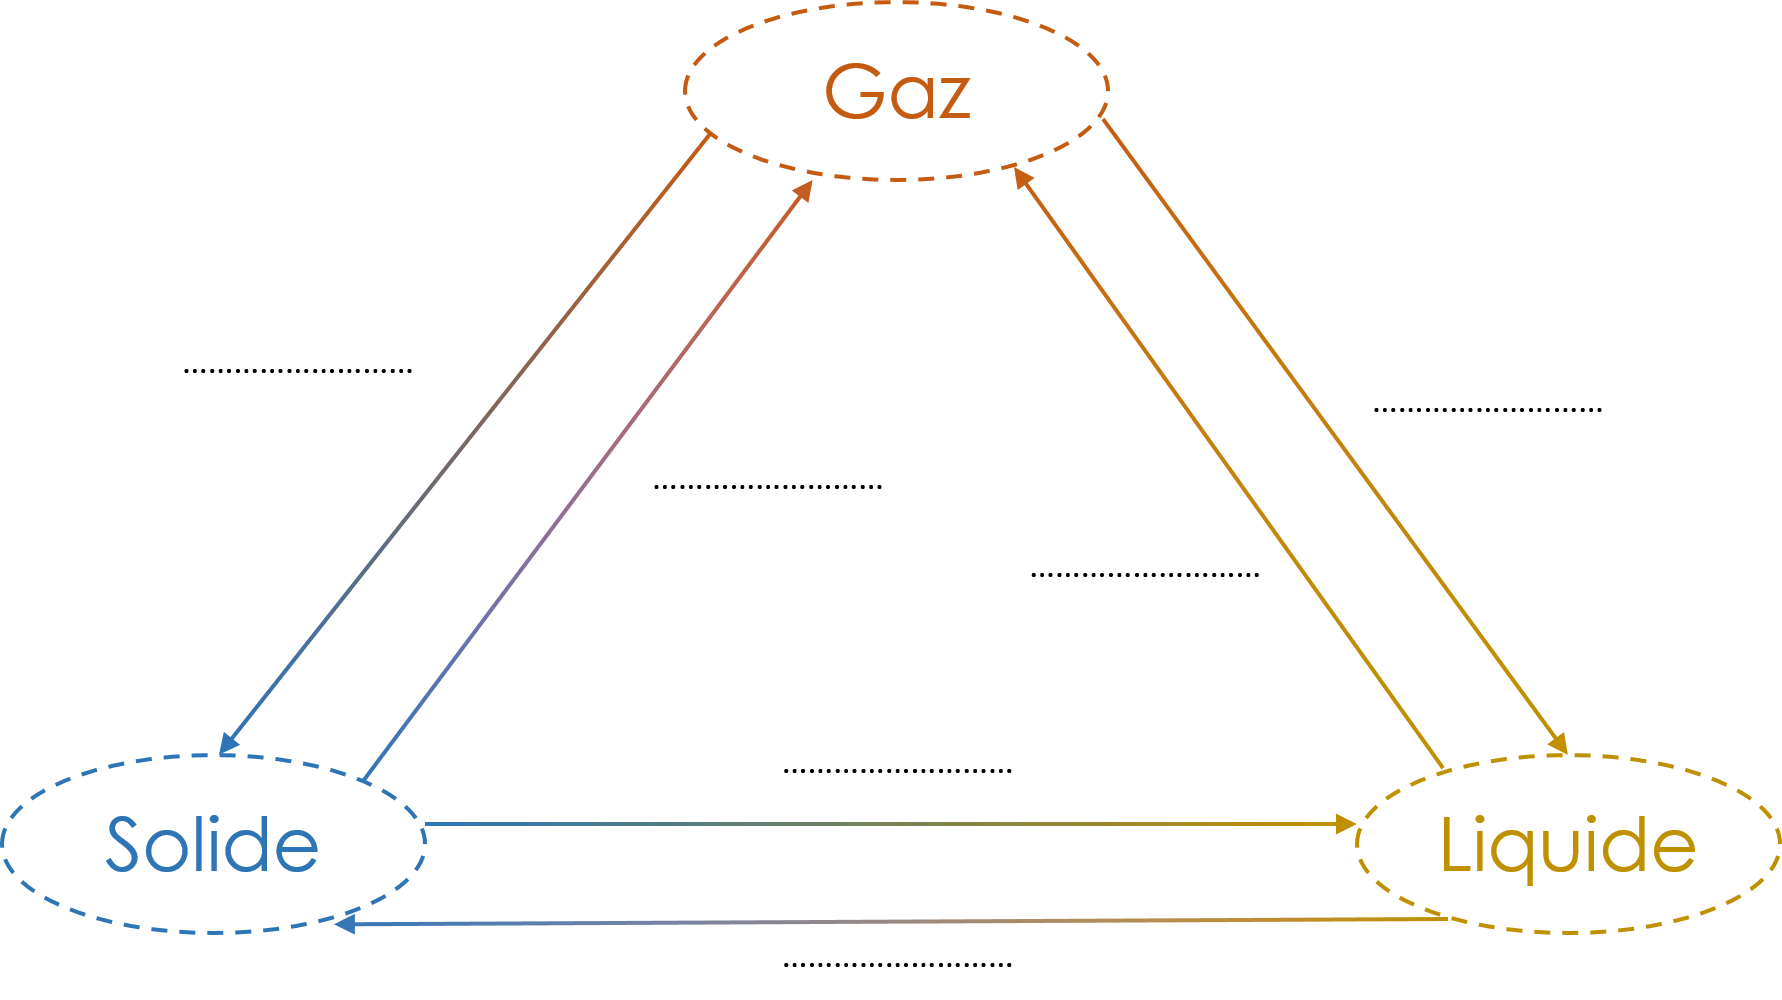
\includegraphics[scale=0.5]{Images/Chapitre_1/Changement_etat.png}
    \caption{Les changements d'états de la matière}
    \label{fig:enter-label}
\end{figure}
Tout changement d'état \underline{d'un corps pur} s'effectue à une température donnée. Il y a deux définitions importantes à connaître :
\begin{itemize}
    \item On appelle \gap{.....................................................}, notée \gap{.........}, d'une espèce chimique la température \textbf{à partir de laquelle la phase solide de cette espèce commence à fondre},
    \item On appelle \textcolor{red}{température d'ébullition}, notée \gap{.........}, d'une espèce chimique la température \textbf{à partir de laquelle la phase liquide de cette espèce commence à s'évaporer.} 
\end{itemize}
On verra en TP qu'on peut mesurer une température de fusion à l'aide d'un \textcolor{red}{banc Kofler}.

\begin{minipage}{0.6\textwidth}
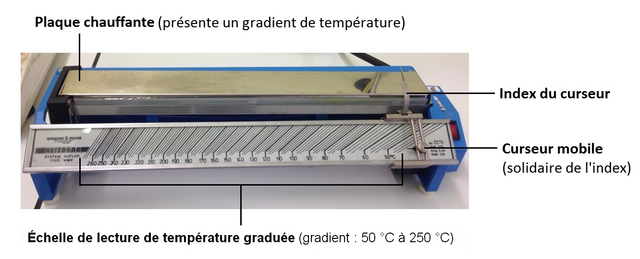
\includegraphics[width=1\textwidth]{Images/Chapitre_1/Banc_Kofler.png} 
  \end{minipage}
\begin{minipage}{0.4\textwidth}
\underline{\textbf{Exemple à connaitre}} :\newline \`{A} une pression de 1~bar, $\theta_{f}(eau)=$ \gap{.......}$\degreCelsius$ et $\theta_{eb}(eau)=$ \gap{.....}$\degreCelsius$
  \end{minipage}



\newpage

\begin{mdframed}[style=autreexo]
\textbf{\bsc{Exercice de cours 4} - Quel état ?}\\
Dans quel état se trouve l'acide citrique à 0~$\degreCelsius$, à température ambiante (20~$\degreCelsius$) et à 100~$\degreCelsius$.\\
\textit{Données :} $\theta_f=153$~$\degreCelsius$ et $\theta_{eb}=310$~$\degreCelsius$
\end{mdframed}
\vspace{2cm}
\subsection{Chromatograhie sur Couche Mince (CCM)}

\begin{tcolorbox}[colback=green!5!white,colframe=green!75!black,title=\textbf{CCM }, upperbox=invisible]
Une chromatographie sur couche mince est une méthode expérimentale permettant de \textbf{séparer} et \textbf{d'identifier} des éléments chimiques différentes d'un mélange homogène.
\newline
\newline 
\newline
\end{tcolorbox}
Elle repose sur la différence d'affinité des espèces chimiques étudiées pour deux phases :
\begin{itemize}
    \item \textbf{la phase fixe} : la plaque chromatographique composée la plupart du temps de silice,
    \item \textbf{une phase mobile} : l'éluant qui va entraîner les espèces à se séparer le long de la phase fixe.
\end{itemize}

\begin{minipage}[c]{0.4\textwidth}
    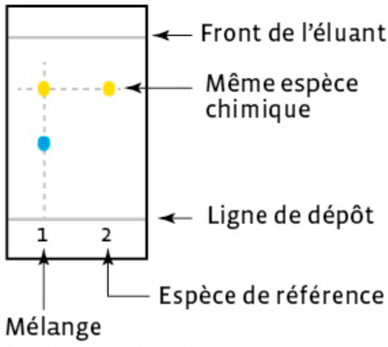
\includegraphics{Images/Chapitre_1/CCM.png}
\end{minipage}
\begin{minipage}[c]{0.6\textwidth}
    \textbf{Lecture d'un chromatogramme} :
    \begin{itemize}
        \item \underline{Lecture horizontale :} deux tâches situées à la même hauteur correspondent à la même espèce chimique. Ce sont les tâchs jaunes sur la figures de gauche.
        \item  \underline{Lecture verticale :} si un dépôt donne plusieurs tâches (comme c'est le cas sur la figure de gauche), alors il est constitué de plusieurs espèces chimiques : c’est un mélange.
    \end{itemize}
\end{minipage}
  %%\newpage
%$ $
%\newpage

\renewcommand{\thesubsection}{\textcolor{red}{\Roman{section}.\arabic{subsection}}}
\renewcommand{\thesubsubsection}{\textcolor{red}{\Roman{section}.\arabic{subsection}.\alph{subsubsection}}}

\setcounter{section}{0}
\sndEnTeteCoursUn

\begin{center}
\begin{mdframed}[style=titr, leftmargin=60pt, rightmargin=60pt, innertopmargin=7pt, innerbottommargin=7pt, innerrightmargin=8pt, innerleftmargin=8pt]

\begin{center}
\large{\textbf{Chapitre 1: Corps purs et mélanges au quotidien}}
\end{center}

\end{mdframed}
\end{center}
Ce chapitre permet de faire une description de la matière à l'échelle macroscopique (c'est-à-dire à notre échelle). Posons-nous les questions suivantes : Qu'est-ce qu'une espèce chimique ? Comment faire pour en identifier une en laboratoire ? Comment reconnaître un mélange d'une espèce chimique unique ?
%
\begin{tcolorbox}[colback=blue!5!white,colframe=blue!75!black,title=Mots clés du chapitre :]
Corps purs, mélange homogène/hétérogène, masse volumique, températures de changement d'état, solubilité.
\end{tcolorbox}

%

\section{Définitions}

\subsection{Espèces chimiques}

La matière est constituée d'\textcolor{red}{entités chimiques} : les atomes, les molécules, les ions. \`{A} partir de ces entités, on peut définir une \textcolor{red}{espèce chimique} :
\begin{tcolorbox}[colback=green!5!white,colframe=green!75!black,title=\textbf{Espèce chimique}, ]
Elle est composée d'un ensemble d'entités chimiques identiques. Une espèce chimique est caractérisée par :
\begin{itemize}
    \item sa formule chimique : par exemple \chemform{H_2O} pour l'eau,
    \item son aspect : couleur, texture, forme, ...
    \item ses propriétés physiques : température d'ébullition, masse volumique, indice de réfraction, ...
    \item ses propriétés chimiques : réactivité avec d'autres espèces chimiques, ... 
\end{itemize}

\end{tcolorbox}

\begin{mdframed}[style=autreexo]
\textbf{\bsc{Exercice de cours 1} - Espèces chimiques}\\
Donner le type (\textit{atomique}, \textit{moléculaire} ou \textit{ionique}) des espèces chimiques suivantes : hélium (He), eau (H\textsubscript{2}O), chlorure de sodium (Na$^{+}$, Cl$^{-}$).
\end{mdframed}
\textit{Réponse :} He : atomique, H\textsubscript{2}O : moléculaire, (Na$^{+}$, Cl$^{-}$) : ionique.

On distingue alors les \textcolor{red}{corps purs} et les \textcolor{red}{mélanges}.

\subsection{Les corps purs}
\begin{tcolorbox}[colback=green!5!white,colframe=green!75!black,title=\textbf{Corps purs}]
Un corps pur est constitué d'une unique espèce chimique.
\end{tcolorbox}

Les corps purs peuvent être :

\begin{itemize}
    \item \textcolor{red}{simples} : ils sont constitués d'un seul type d'atome. Exemples : le dihydrogène \chemform{H_2}, le charbon \chemform{C}, l'argent \chemform{Ag}.
    \item \textcolor{red}{composés} : ils sont constitués de plusieurs atomes dans des proportions bien définies. Exemples : l'eau \chemform{H_2O}, l'éthanol \chemform{C_2H_6O}, le chlorure de sodium \chemform{(Na^+;Cl^-)}.
\end{itemize}

%%%%%%%%



%
\subsection{Le cas des mélanges}
\begin{tcolorbox}[colback=green!5!white,colframe=green!75!black,title=\textbf{Mélange}]
Un mélange est constitué de plusieurs espèces chimiques différentes.
\end{tcolorbox}
Les mélanges peuvent être :
\begin{itemize}
    \item \textcolor{red}{homogènes} : ils sont constitués d'une seule phase (solide, liquide ou vapeur) indiscernable à l'\oe il nu. Lorsque deux liquides se mélangent l'un avec l'autre, on dit qu'ils sont \textcolor{red}{miscibles}.
    \item \textcolor{red}{hétérogènes} : ils sont constitués de plusieurs phases discernables à l'\oe il nu.
\end{itemize}

\begin{mdframed}[style=autreexo]
\textbf{\bsc{Exercice de cours 2} - Corps purs et mélanges}\\
Pour chaque substance suivante, dire s’il s’agit d’un corps pur simple/complexe ou d’un mélange homogène/hétérogène.
\end{mdframed}
\begin{table*}
    \centering
    \begin{tabular}{|C{0.15}|C{0.15}|c|c|C{0.15}|}
    \hline
    Description & Bécher d'huile et d'eau & Bécher d'huile & Bécher d'eau pure & Bécher d'azote liquide \\
    \hline
    Photographie & 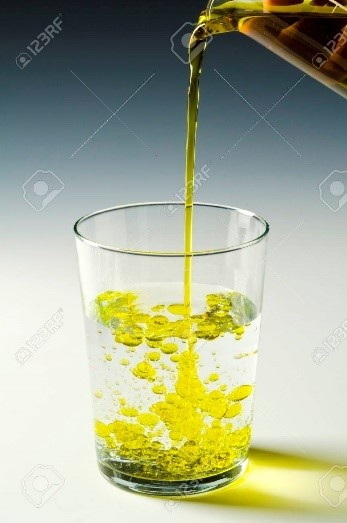
\includegraphics[scale=0.6]{Images/Chapitre_1/Becher_huile_eau.jpg} & 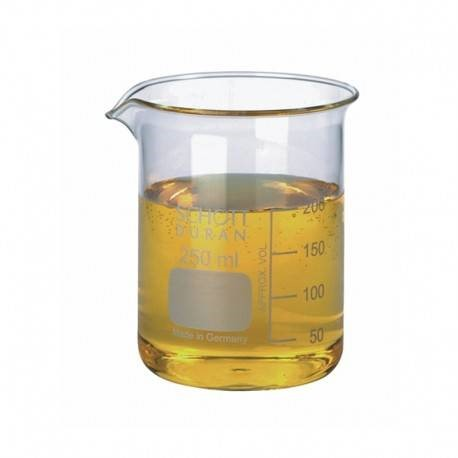
\includegraphics[scale=0.3]{Images/Chapitre_1/Becher_huile.jpg} & 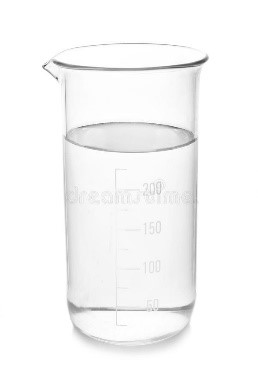
\includegraphics[scale=0.7]{Images/Chapitre_1/Becher_eau.jpg} & 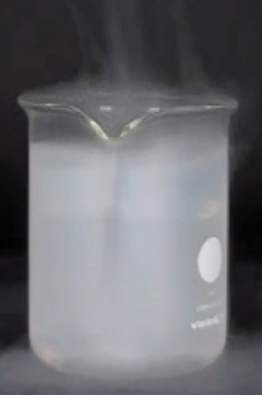
\includegraphics[scale=0.3]{Images/Chapitre_1/Becher_azote.png} \\
    \hline
    Type de corps &  &  &  & \\
    \hline
    Qualificatif du corps & & & &  \\
    \hline
   \end{tabular}
\end{table*}

\section{Identification d'espèces chimiques}
Comment reconnaitre expérimentalement une espèce chimique par rapport à une autre ? On présente dans cette partie quelques éléments qui vont nous permettre de répondre à cette question.

\subsection{Tests chimiques}
\begin{tcolorbox}[colback=red!5!white,colframe=red!75!black,title=\textbf{Tests chimiques à connaître : }]
%\begin{table}
    %\centering
   \begin{tabular}{|C{0.31}|C{0.3}|C{0.31}|}
   \hline
    \cellcolor{blue!25} Espèce chimique à tester & \cellcolor{blue!25} Test & \cellcolor{blue!25} Résultat du test positif \\
    \hline
    Eau (\chemform{H_2O}) & Sulfate de cuivre anhydre (solide blanc)  & Apparition d'un précipité bleu \\
    \hline
    Dioxygène (\chemform{O_2}) & Bûche incandescente & La bûche s'enflamme, incandescence ravivée \\
    \hline
    Dihydrogène (\chemform{H_2}) & Allumette enflammée  &  Détonation \\
    \hline 
    Dioxyde de carbone (\chemform{CO_2}) & Eaux de chaux & Eau de chaux troublée, un précipité blanc appararaît \\
    \hline
    \end{tabular}
%\end{table}
\end{tcolorbox} 

\subsection{Propriétés physiques}
\subsubsection{La masse volumique}
\begin{tcolorbox}[colback=green!5!white,colframe=green!75!black,title=\textbf{Rappel : masse volumique et densité }]
La masse volumique d'une espèce chimique est :
\begin{equation*}
    \rho = \frac{m}{V}
\end{equation*}
avec m la masse de l'espèce et V son volume. Elle s'exprime en g.cm$^{-3}$.\\
La densité $d$ d'une espèce chimique est le rapport entre la masse volumique de cette substance et la masse volumique de l'eau liquide valant $\rho_{eau}=1$~g.cm$^{-3}$ :
\begin{equation*}
    d = \frac{\rho_{espece}}{\rho_{eau}}
\end{equation*}
\importantbox{$d$ s'exprime sans unité puisqu'il s'agit d'un rapport entre deux grandeurs physique de même nature.}
\end{tcolorbox}

\begin{tcolorbox}[colback=red!5!white,colframe=red!75!black,title=\textbf{Masse volumique de l'eau: }]
\begin{center}
    $\rho_{eau} = $1000~kg.m$^{-3}$ ou 1~g.cm$^{-3}$. 
\end{center}
\end{tcolorbox}

\begin{tabular}{|c|C{0.06}|C{0.06}|C{0.06}|C{0.1}|C{0.15}|C{0.1}|C{0.1}|}
   \hline
     & Vide & Air & Eau & Glace & Cyclohexane & Bronze & Or \\
    \hline
    $\rho$ (en g.cm$^{-3}$) & 0 & 0,001 & 1,0 & 0,92 & 0,79 & 7,9 & 19  \\
    \hline
    d & 0 & 0,001 & 1,0 & 0,92 & 0,79 & 7,9 & 19 \\
    \hline
    \end{tabular}
\begin{mdframed}[style=autreexo]
\textbf{\bsc{Exercice de cours 3} - Masse volumique du cyclohexane}\\
\textbf{1)} Calculer la masse volumique du cyclohexane sachant qu'un volume de 15~mL a une masse de 11,8~g.\newline \textbf{2)} Le cyclohexane est-il plus dense que l'eau ? \end{mdframed}
\textit{Réponse :} \\
\textbf{1)}. On calcule la masse volumique du cyclohexane à l'aide de la formule du cours : $\rho=\frac{m}{V} = \frac{11,8}{15}=0,79$~g.mL$^{-1}=0,79$ g.cm$^{-3}$.\\
\textbf{2)}. On déduit la densité à l'aide de la formule du cours et de la question 1) : $d=\frac{\rho_{cyclohexane}}{\rho_{eau}}=\frac{0,79}{1,0}=0,79$. Comme $d<1$, le cyclohexane est moins dense que l'eau. 
\newpage

\subsubsection{Les températures de changement d'état}
\begin{figure}[!htb]
    \centering
    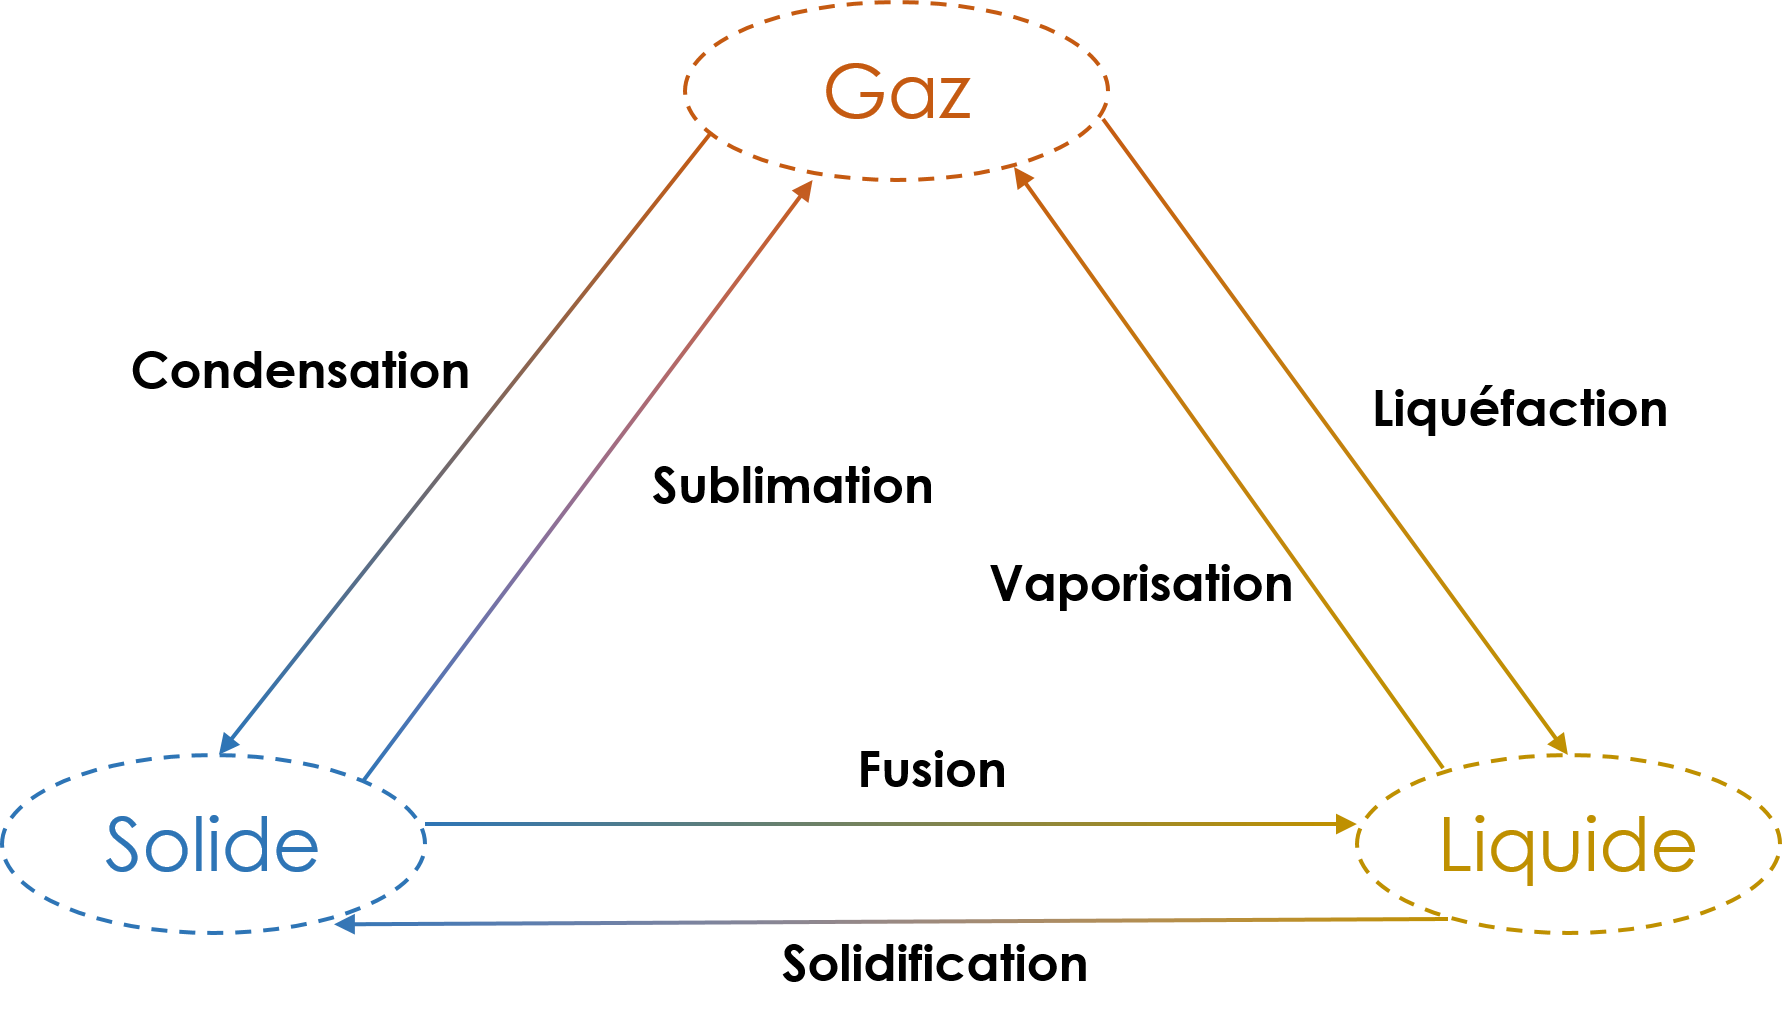
\includegraphics[scale=0.5]{Images/Chapitre_1/Changement_etat_complet.png}
    \caption{Les changements d'états de la matière}
    \label{fig:enter-label}
\end{figure}
Tout changement d'état \underline{d'un corps pur} s'effectue à une température donnée. Il y a deux définitions importantes à connaître :
\begin{itemize}
    \item On appelle \textcolor{red}{température de fusion}, notée $\theta_f$, d'une espèce chimique la température \textbf{à partir de laquelle la phase solide de cette espèce commence à fondre},
    \item On appelle \textcolor{red}{température d'ébullition}, notée $\theta_{eb}$, d'une espèce chimique la température \textbf{à partir de laquelle la phase liquide de cette espèce commence à s'évaporer.} 
\end{itemize}
On verra en TP qu'on peut mesurer une température de fusion à l'aide d'un \textcolor{red}{banc Kofler}.

\begin{minipage}{0.6\textwidth}
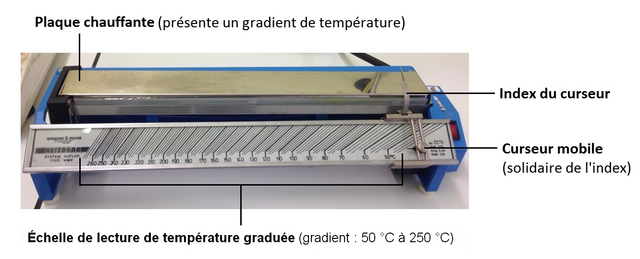
\includegraphics[width=1\textwidth]{Images/Chapitre_1/Banc_Kofler.png} 
  \end{minipage}
\begin{minipage}{0.4\textwidth}
\underline{\textbf{Exemple à connaitre}} :\newline \`{A} une pression de 1~bar, $\theta_{f}(eau)=0\degreCelsius$ et $\theta_{eb}(eau)=100\degreCelsius$
  \end{minipage}



\newpage

\begin{mdframed}[style=autreexo]
\textbf{\bsc{Exercice de cours 4} - Quel état ?}\\
Dans quel état se trouve l'acide citrique à 0~$\degreCelsius$, à température ambiante (20~$\degreCelsius$) et à 100~$\degreCelsius$.\\
\textit{Données :} $\theta_f=153$~$\degreCelsius$ et $\theta_{eb}=310$~$\degreCelsius$
\end{mdframed}
\textit{Réponse :} Les trois températures 0~$\degreCelsius$, 20~$\degreCelsius$ et 100~$\degreCelsius$ sont inférieures à la température de fusion $\theta_f=153$~$\degreCelsius$ de l'acide citrique. Ce dernier est donc solide à ces températures.

\subsection{Chromatograhie sur Couche Mince (CCM)}

\begin{tcolorbox}[colback=green!5!white,colframe=green!75!black,title=\textbf{CCM }]
Une chromatographie sur couche mince est une méthode expérimentale permettant de \textbf{séparer} et \textbf{d'identifier} des éléments chimiques différentes d'un mélange homogène.
\end{tcolorbox}
Elle repose sur la différence d'affinité des espèces chimiques étudiées pour deux phases :
\begin{itemize}
    \item \textbf{la phase fixe} : la plaque chromatographique composée la plupart du temps de silice,
    \item \textbf{une phase mobile} : l'éluant qui va entraîner les espèces à se séparer le long de la phase fixe.
\end{itemize}

\begin{minipage}[c]{0.4\textwidth}
    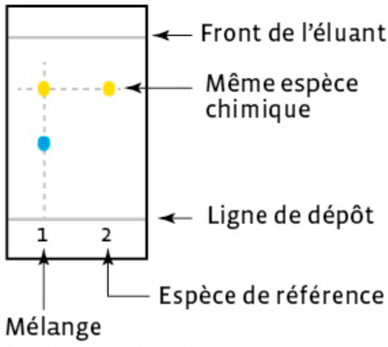
\includegraphics{Images/Chapitre_1/CCM.png}
\end{minipage}
\begin{minipage}[c]{0.6\textwidth}
    \textbf{Lecture d'un chromatogramme} :
    \begin{itemize}
        \item \underline{Lecture horizontale :} deux tâches situées à la même hauteur correspondent à la même espèce chimique. Ce sont les tâchs jaunes sur la figures de gauche.
        \item  \underline{Lecture verticale :} si un dépôt donne plusieurs tâches (comme c'est le cas sur la figure de gauche), alors il est constitué de plusieurs espèces chimiques : c’est un mélange.
    \end{itemize}
\end{minipage}

\section{Composition d'un mélange}
On vient de voir dans la partie précédente comment identifier une ou plusieurs espèces chimiques en fonction de ses propriétés physico-chimiques. Mais comment donne-t'on la composition d'un mélange ? On introduit ici la proportion volumique et massique d'une espèce dans un mélange.

\subsection{Proportion volumique et massique}

\begin{tcolorbox}[colback=green!5!white,colframe=green!75!black,title=\textbf{Proportion volumique}]
La proportion en volume (ou volumique) d'une espèce dans un mélange est le quotient du volume $V_{E}$ qu'occupe cette espèce par le volume total $V_{tot}$ du mélange :
\begin{equation*}
    \frac{V_E}{V_{tot}}
\end{equation*}
avec $V_{E}$ et $V_{tot}$ exprimées dans la même unité (L ou m$^3$ par exemple)
\end{tcolorbox}

\begin{tcolorbox}[colback=green!5!white,colframe=green!75!black,title=\textbf{Proportion massique}]
La proportion en masse (ou massique) d'une espèce dans un mélange est le quotient de la masse $m_{E}$ de cette espèce dans le mélange par la masse totale $m_{tot}$ du mélange :
\begin{equation*}
    \frac{m_E}{m_{tot}}
\end{equation*}
avec $m_{E}$ et $m_{tot}$ exprimées dans la même unité (g ou kg par exemple).
\end{tcolorbox}

Ces proportions peuvent être exprimées en \% et sont sans unités puisqu'il s'agit d'un rapport en deux grandeurs sans unités.

\subsection{Exemple à connaître : la composition de l'air}
L'air est un mélange de gaz indispensable à la vie sur Terre. Quand il est sec, c'est-à-dire qu'il ne contient pas de vapeur d'eau, voici sa composition :
\begin{figure}[!hbt]
    \centering
    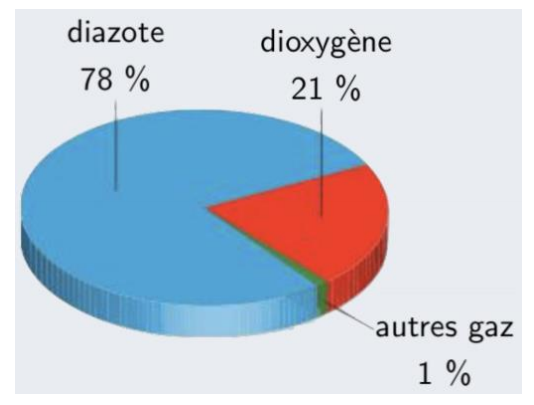
\includegraphics[scale=0.5]{Images/Chapitre_1/Composition_air.png}
    \caption{Diagramme de la composition de l'air}
    \label{fig:compo_air}
\end{figure}

\begin{mdframed}[style=autreexo]
\textbf{\bsc{Exercice de cours 5} - Proportion}\\
A partir du diagramme présenté sur la figure, donnez le volume occupé par le diazote et le dioxygène pour un volume d'air total de $100$~L.
\end{mdframed}
\textit{Réponse :} Diazote : $V_{N_2}=78\%*100=78$~L. Dioxygène : $V_{O_2}=21\%*100=21$~L.


  %\renewcommand{\thesubsection}{\textcolor{red}{\Roman{section}.\arabic{subsection}}}
\renewcommand{\thesubsubsection}{\textcolor{red}{\Roman{section}.\arabic{subsection}.\alph{subsubsection}}}

\setcounter{section}{0}
\sndEnTeteDeux

\begin{center}
\begin{mdframed}[style=titr, leftmargin=60pt, rightmargin=60pt, innertopmargin=7pt, innerbottommargin=7pt, innerrightmargin=8pt, innerleftmargin=8pt]

\begin{center}
\large{\textbf{Feuille d'exercices du Chapitre 1}}
\end{center}

\end{mdframed}
\end{center}

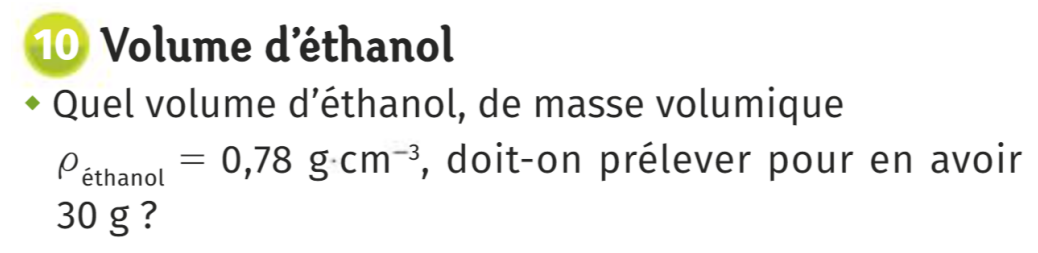
\includegraphics[scale=0.9]{Images/Chapitre_1/Exo_1_Chap1.png}
\vspace{1cm}

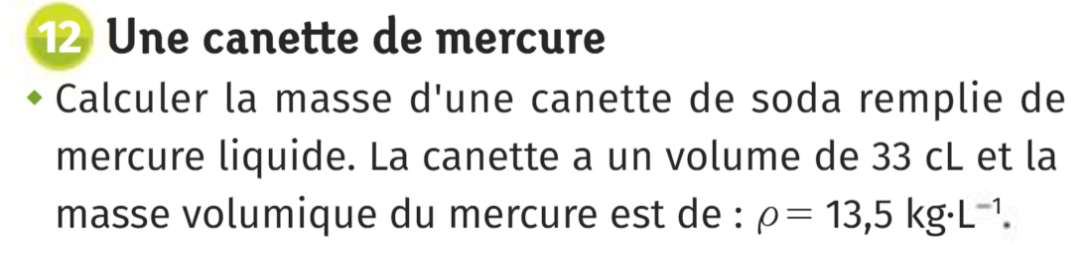
\includegraphics[scale=0.9]{Images/Chapitre_1/Exo_2_Chap1.png}
\vspace{1cm}

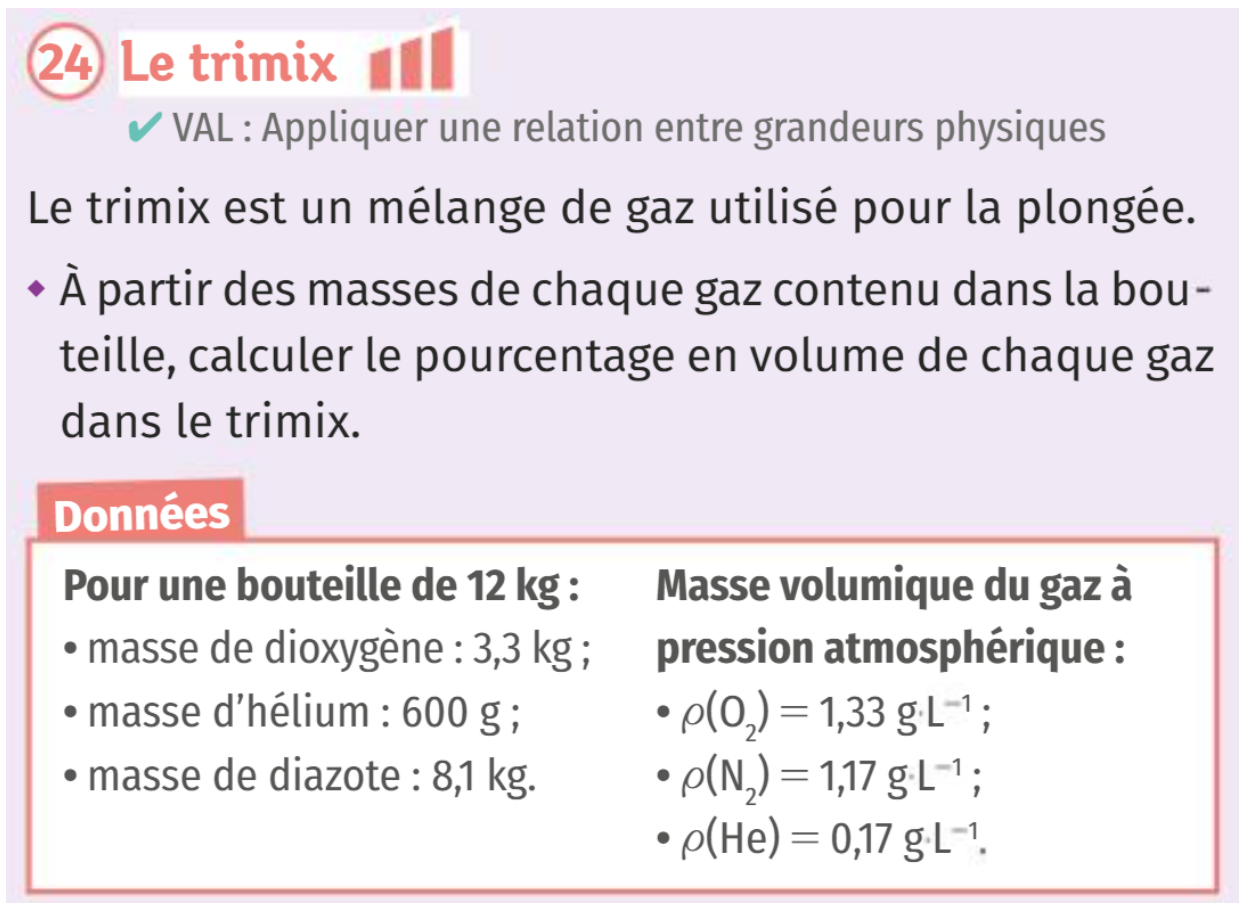
\includegraphics[scale=0.7]{Images/Chapitre_1/Exo_5_Chap1.png}
\vspace{1cm}

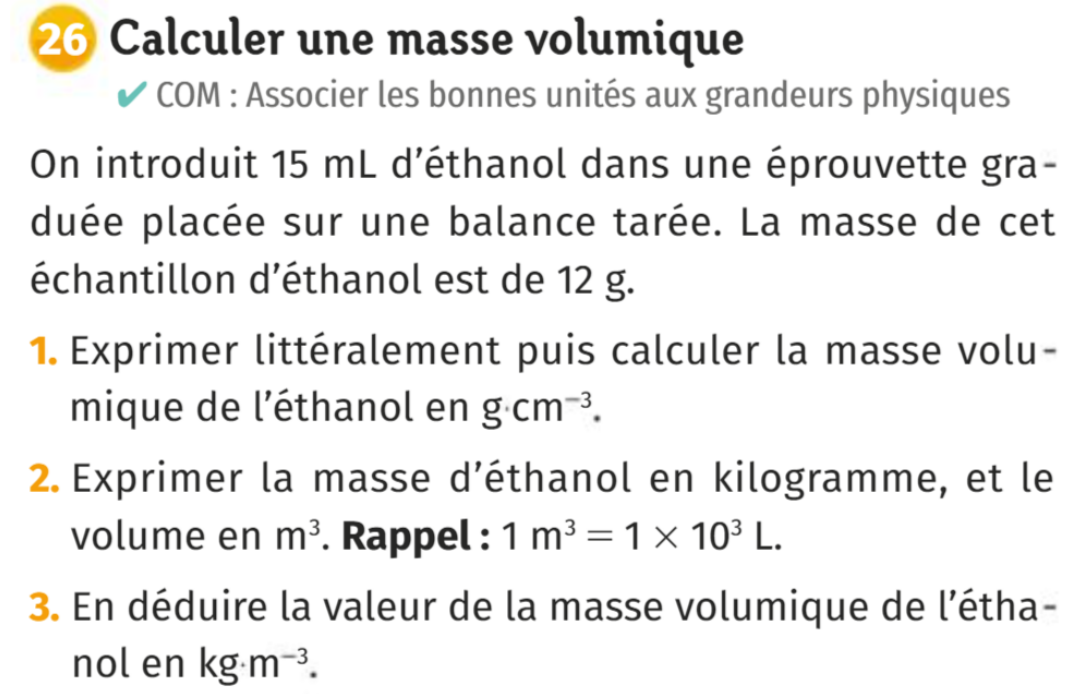
\includegraphics[scale=0.8]{Images/Chapitre_1/Exo_3_Chap1.png}
\vspace{1cm}

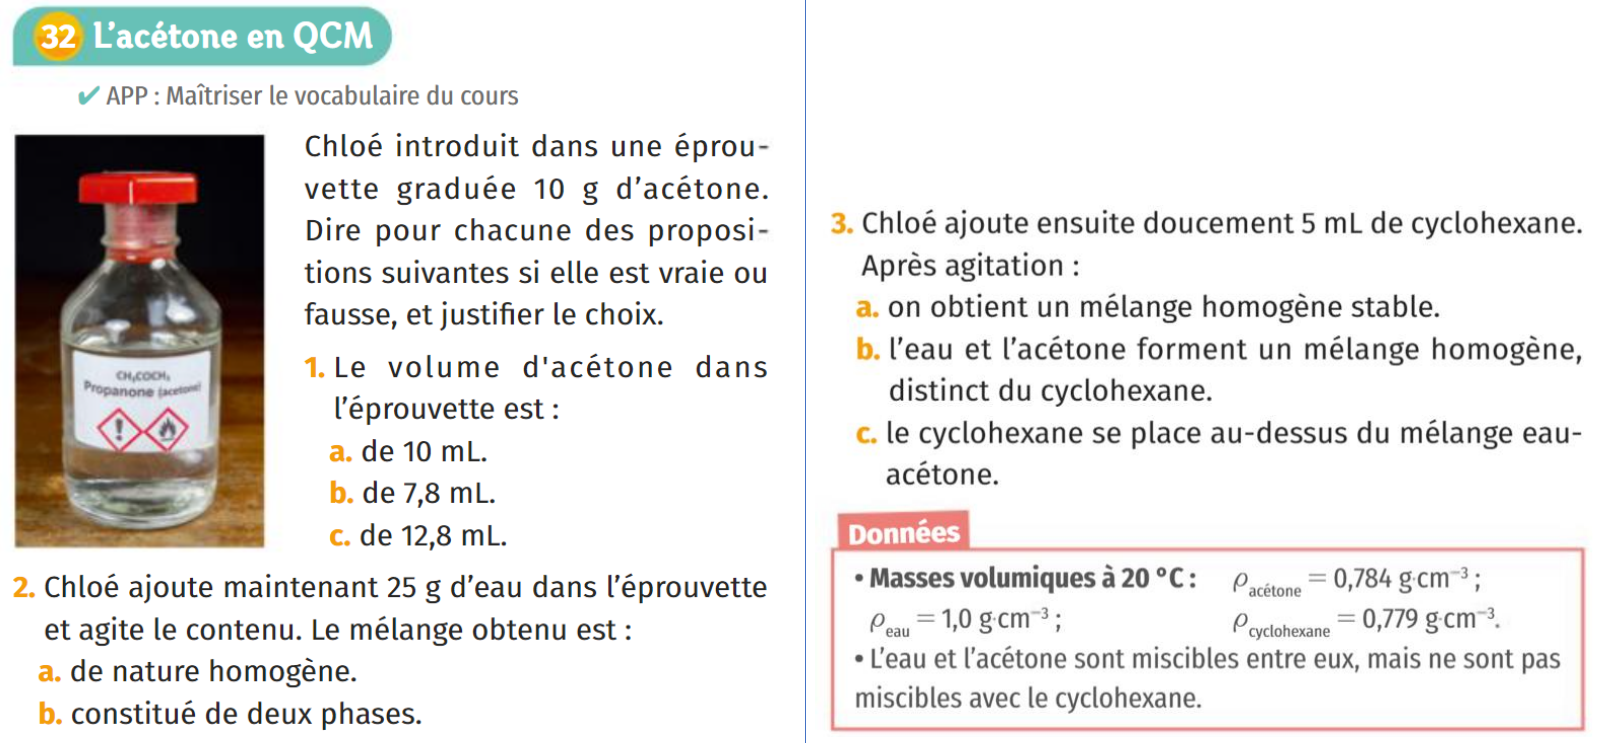
\includegraphics[scale=0.6]{Images/Chapitre_1/Exo_6_Chap1.png}
\vspace{1cm}

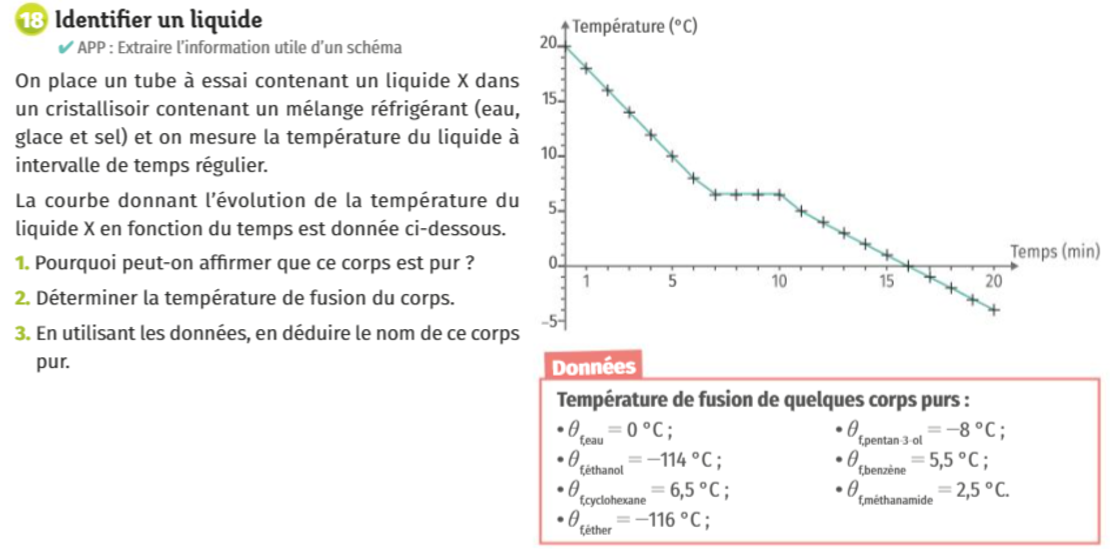
\includegraphics[scale=1]{Images/Chapitre_1/Exo_7_Chap1.png}


  %\newpage

\renewcommand{\thesubsection}{\textcolor{red}{\Roman{section}.\arabic{subsection}}}
\renewcommand{\thesubsubsection}{\textcolor{red}{\Roman{section}.\arabic{subsection}.\alph{subsubsection}}}

\setcounter{section}{0}
\sndEnTeteMethodoUn

\begin{center}
\begin{mdframed}[style=titr, leftmargin=60pt, rightmargin=60pt, innertopmargin=7pt, innerbottommargin=7pt, innerrightmargin=8pt, innerleftmargin=8pt]

\begin{center}
\large{\textbf{Fiche méthode 1 : Outils pour la Physique et la Chimie}}
\end{center}

\end{mdframed}
\end{center}
Ce chapitre présente quelques rappels sur les outils mathématiques, les méthodes et les représentations que nous utiliserons toute l'année en physique comme en chimie. Il est donc essetiel de maîtriser ces notions pour démarrer l'année sur d'excellentes bases. N'hésitez pas à le reconsulter toute l'année au besoin !

\begin{tcolorbox}[colback=blue!5!white,colframe=blue!75!black,title=Mots clés du chapitre :]
Puissance de $10$, unités SI, règles de sécurité en chimie
\end{tcolorbox}

\section{Puissance de 10}
\subsection{Représentation}
Les nombres très grands ou très petits s'écrivent à l'aide des puissances de 10 :
\begin{align*}
    10^n &= \underbrace{10\times10\times ... \times 10}_{\text{\textbf{n} "10 $\times$"}} = 1\underbrace{00...0}_{\text{\textbf{n} zéros}} \\
    10^{-n} &= \frac{1}{10^n} = 0,0....0\underbrace{1}_{\text{en \textbf{n-ième} position}}
\end{align*}

\underline{Exemples :} $10^9$ = 1 000 000 000,    $10^{-5}$=0,000 01\\

\subsection{Opérations}
\begin{tcolorbox}[colback=red!5!white,colframe=red!75!black,title=\textbf{Règles de calculs des puissances de 10}]
Soit $a$ et $b$ deux nombres réels.
\begin{align*}
    10^{a}\times 10^b &= 10^{a+b} & \text{Ex :}& 10^{1}\times 10^2 = 10^{1+2}=10^3 \\
    \frac{10^{a}}{10^b} &= 10^{a-b} & \text{Ex :}& \frac{10^{1}}{10^2} = 10^{1-2}=10^{-1} \\
\end{align*}

\end{tcolorbox}
\underline{Effectuer les calculs suivants :}
\begin{align*}
    10^{30} \times 10^{50} &= 10^{30+50}=10^{80} & \frac{10^{2033}}{10^{10}} &= 10^{2033-10} = 10^{2023} & \frac{10^2}{10^8}\times 10^5 &= 10^{2-8+5} = 10^{-1}
\end{align*}
\subsection{Notation scientifique}

\begin{tcolorbox}[colback=green!5!white,colframe=green!75!black,title=\textbf{Ecriture scientifique d'un nombre}]
En écriture scientifique, une valeur numérique s'exprime sous la forme :
\begin{equation*}
    a \times 10^n
\end{equation*}
avec $n$ un nombre entier relatif et $a$ un nombre décimal tel que : $1< a <10$.\\
\\
\end{tcolorbox}
\underline{Exemples :}
\begin{itemize}
    \item la masse $M_{L}$ de la Lune vaut $M_{Lune}=734$ $800$ $000$ $000$ $000$ $000$ $000$~kg et s'écrit donc plus simplement : $M_L=7,348\times 10^{20}$~kg
    \item La taille $d$ d'une molécule d'eau est de  $d=0,000$ $000$ $003$ $4$~m, soit en écriture scientifique : $d=3,4\times10^{-9}$~m
\end{itemize}

\subsection{Ordre de grandeur}
\begin{tcolorbox}
[colback=green!5!white,colframe=green!75!black,title=\textbf{Ordre de grandeur d'un nombre}]
L'ordre de grandeur d'un nombre et la puissance de 10 la plus proche de ce nombre.
\end{tcolorbox}
\underline{Exemples :}
\begin{itemize}
    \item Ordre de grandeur de 30 000 = 10$^4$
    \item Ordre de grandeur de 0,000 007 = 10$^{-5}$
    \item Ordre de grandeur de 8 700 000 = 10$^6$
    \item Ordre de grandeur de 0,000 256 = 10$^{-4}$
\end{itemize}

\section{Unités}
\subsection{Les unités du système international SI}
Depuis 2019, la communauté scientifique internationale, à travers la "Conférence générale des poids et mesures", a adopté un système d'unités universel. Leur valeur sont définies à partir de 7 constantes universelles dont les valeurs exactes ont été définitivement "fixées" en Novembre 2018 (\textit{source Wikipédia}). 
\begin{figure}[!h]
    \centering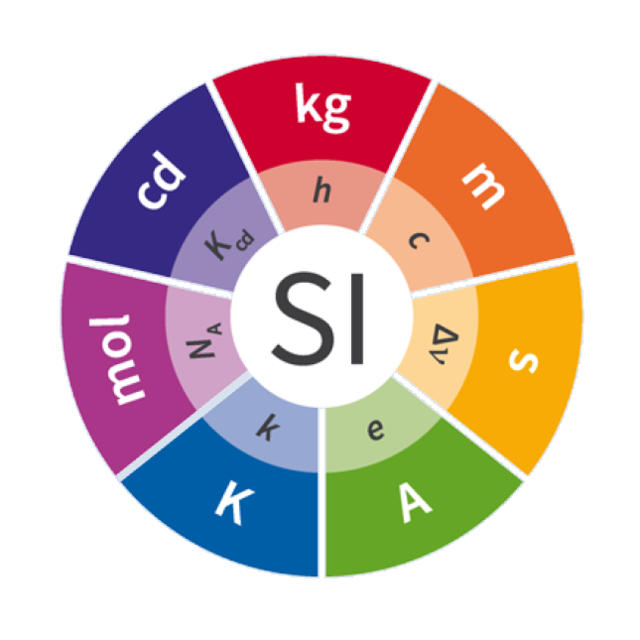
\includegraphics[scale=0.4]{Images/Methodo/Fiche_Methode1/SI_Logo_with_defining_constants.png}
    \caption{Logo du système SI. }
    \label{fig:Syteme_SI}
\end{figure}
\begin{table}[!h]
    \centering
    \begin{tabularx}{\textwidth}{| X | X | c | X |}  \hline
Grandeur physique & Unité SI & Symbole de l'unité & Appareil de mesure \\
\hline
Masse & kilogramme & kg & balance \\
Temps & seconde & s & chronomètre \\
Longueur & mètre & m & règle \\
Température & kelvin & K & thermomètre \\
Intensité électrique & ampère & A & ampèremètre \\
Quantité de matière & mole & mol & balance\\
Intensité lumineuse & candela & cd & luxmètre \\
\hline
\end{tabularx}
    \caption{Tableau des unités du SI et les appareils de mesure associés.}
    \label{tab:SI}
\end{table}
\importantbox{Nous utilisons courament d'autres unités qui nous paraissent bien plus pratiques dans leur utilisation. Par exemple, nous utilisons plus facilement les degrés celsius $^\circ$C pour la température ou encore les tailles XS, S, M, L, ... pour les vêtements (même si la relation entre ces dernières \og unités \fg et les unités du SI semble très obscure...).}


\subsection{Préfixes des unités.}
Il est très souvent utile et agréable de remplacer l’écriture scientifique d’un nombre par \textbf{un nombre écrit sans puissance de 10 suivi d'un multiple ou sous-multiple de l'unité du nombre}.
\begin{table}[!h]
    \centering
    \begin{tabular}{|C{0.15}|c|c|}
    \hline
    Multiple ou sous-multiple & Facteur par lequel l'unité est multipliée & Exemple typique \\ 
    \hline 
    Multiple & 1 000 000 000 000 = $10^{12}$ & Téraoctet (To) \\
    \hline
    Multiple & 1 000 000 000 = $10^{9}$ & Gigaoctet (Go)\\
    \hline
    Multiple & 1 000 000 = $10^{6}$ & Mégajoule (MJ)\\
    \hline
    Multiple & 1 000 = $10^{3}$ & kilogramme (kg)\\
    \hline
    Multiple & 100 = $10^{2}$ & hectomètre (hm)\\
    \hline
    Multiple & 10 = $10^{1}$ &  decalitre (daL)\\
    \hline
    Sous-Multiple & 0,1 = $10^{-1}$ & decimètre (dm) \\
    \hline
    Sous-Multiple & 0, 01 = $10^{-2}$ & centilitre (cL) \\
    \hline
    Sous-Multiple & 0, 001 = $10^{-3}$ & milliseconde (ms) \\
    
    \hline
    Sous-Multiple & 0, 000 001 = $10^{-6}$ & micromètre ($\mu$m)\\
    \hline
    Sous-Multiple & 0, 000 000 001 = $10^{-9}$ & nanoseconde (ns) \\
    \hline
    Sous-Multiple & 0, 000 000 000 001 = $10^{-12}$ & picomètre (pm)\\
    \hline
    Sous-Multiple & 0, 000 000 000 000 001 = $10^{-15}$ & femtomètre (fm)\\
    \hline
    \end{tabular}
    
    \caption{Tableaux des préfixes des multiples et sous multiples}
    \label{tab:chap1_multiples}
\end{table}

\section{Chiffres significatifs}

\begin{tcolorbox}
[colback=green!5!white,colframe=green!75!black,title=\textbf{Chiffre significatif}]
Lorsqu’on écrit une valeur en notation scientifique, le nombre de chiffres employés dans le facteur avant la puissance de 10 est le nombre de chiffres significatifs.\\
\end{tcolorbox}
Exemples : 
\begin{itemize}
    \item la célérité de la lumière $c$ dans le vide est :
\begin{equation*}
    c =\underbrace{2,99 792458}_{\text{9 chiffres significatifs}}\times 10^8~\text{m.s}^{-1}
\end{equation*}
\item 0,002 3 possède 2 chiffres significatifs car il s'écrit : $2,3\times10^{-3}$ en notation scientifique.
\end{itemize}

\begin{tcolorbox}[colback=red!5!white,colframe=red!75!black,title=Règles à retenir sur les chiffres significatifs]
Le résultat d'une somme, différence, produit ou quotient est écrit avec \textbf{le plus petit nombre de chiffres signifcatifs présents dans les grandeurs dans son calcul}.
\newline
\newline
\textit{Exemple : } Calculer le temps $\Delta t$ pour que la lumière parcourt la distance Terre-Soleil $d=150\times 10^{6}$~km. Attention à mettre les grandeurs dans les bonnes unités.
\end{tcolorbox}


\section{Rédaction d'un calcul}
La réponse à une question demandant un calcul ne se résume pas l'invocation simple d'une formule non commentée et un résultat sans unité (à part bien sûr si le résultat attendu est sans unité). A chaque étape, on doit répondre de manière argumentée et présentable un calcul. Prenons l'exemple suivant : 

\begin{mdframed}[style=autreexo]
\textbf{\bsc{Exercice} - Distance Paris-Brest en train}\\
 Un TGV roule à une vitesse de l'ordre de $3,0\times 10^{2}$~km/h en France. La distance entre Paris et Brest est de 580 km.
\begin{enumerate}
\item En combien de temps une voiture roulant en moyenne à $100$~km/h effectue-t-elle ce trajet ?
\item Et un TGV ?
\end{enumerate}
\end{mdframed}

\begin{minipage}{0.5\textwidth}
    \begin{tcolorbox}[colback=red!5!white,colframe=red!75!black,title=\textbf{Mauvaise rédaction : }]
    \textbf{1)} 5,80 \\
    \textbf{2)} 1,93333333\\
    \end{tcolorbox}
\end{minipage}
\begin{minipage}{0.5\textwidth}
    \begin{tcolorbox}[colback=green!5!white,colframe=green!75!black,title=\textbf{Bonne rédaction : }]
    \textbf{1)} Le temps de parcours est donné par la formule $\Delta t=\frac{d}{v}$ avec $d$ la distance Paris-Brest et $v$ la vitesse de la voiture. Avec les données de l'énoncé, on obtient un temps de parcourt pour la voiture de :
    \begin{equation*}
        \Delta t = \frac{580}{100} = 5,8~\text{h}
    \end{equation*}
    \textbf{2)} En utilisant la même formule que la question précédente, on obtient un temps de parcourt pour le TGV de :
     \begin{equation*}
        \Delta t = \frac{580}{3,0\times 10^2} = 1,9~\text{h}
    \end{equation*}
    \end{tcolorbox}
\end{minipage}


\section{Règles de sécurité en TP de chimie}
\subsection{Les règles de sécurité}
\begin{tcolorbox}[colback=red!5!white,colframe=red!75!black,title=\textbf{En TP de chimie :}]
\begin{itemize}
    \item Je porte les EPI (Equipements de Protection Individuel) le cas échéant ;
    \item On ne jette pas les produits chimiques dans le lavabo sauf contre-indication ;
    \item On ne respire pas, ne mange pas et ne boit pas un produit chimique (même si comestible !) ;
    \item On fait attention/respecte le matériel ;
    \item On vérifie les pictogrammes de sécurité lorsqu'on manipule un produit chimique ;
    \item On range et nettoie son plan de travail à la fin du TP ;
\end{itemize}
\end{tcolorbox}

\subsection{Les pictogrammes de sécurité et EPI}
\begin{figure}[!h]
    \centering
    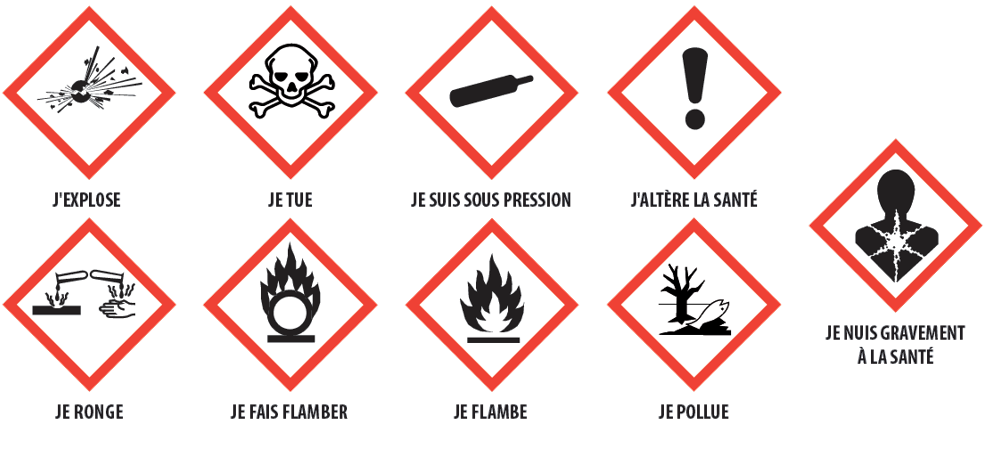
\includegraphics[scale=1]{Images/Methodo/Fiche_Methode1/Pictogrammes.png}
    \caption{Pictogrammes de sécurité}
    \label{fig:enter-label}
\end{figure}

\begin{figure}[!h]
    \centering
    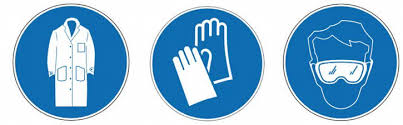
\includegraphics[scale=0.9]{Images/Methodo/Fiche_Methode1/picto_gant_blouse_lunette.jpg}
    \caption{Logo des \'{E}quipements de Protection Individuelle (EPI)}
    \label{fig:enter-label}
\end{figure}

\importantbox{Si vous avez un doute concernant un produit non étiquetté, il ne faut pas hésiter à regarder sa fiche de données de sécurité sur le site de l'INRS (Institut National de Recherche et de Sécurité) : \url{https://www.inrs.fr/publications/bdd/fichetox.html}}

\underline{\textbf{Exemple :}}
\begin{figure}[!h]
    \centering
    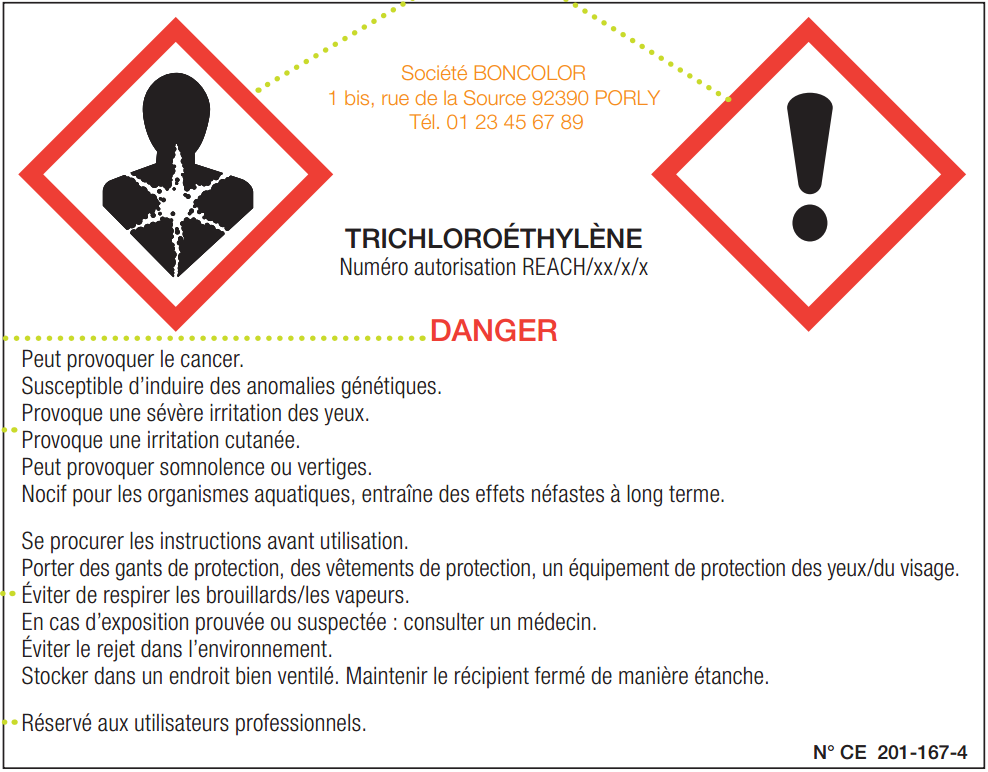
\includegraphics[scale=0.7]{Images/Methodo/Fiche_Methode1/Exemple_fiche_toxico.PNG}
    \caption{Exemple d'une fiche de données de sécurité sur)àoi le site de l'INRS.}
    \label{fig:enter-label}
\end{figure}


  %%\newpage
%$ $
%\newpage

\renewcommand{\thesubsection}{\textcolor{red}{\Roman{section}.\arabic{subsection}}}
\renewcommand{\thesubsubsection}{\textcolor{red}{\Roman{section}.\arabic{subsection}.\alph{subsubsection}}}

\setcounter{section}{0}
\sndEnTeteTPUn

\begin{center}
\begin{mdframed}[style=titr, leftmargin=60pt, rightmargin=60pt, innertopmargin=7pt, innerbottommargin=7pt, innerrightmargin=8pt, innerleftmargin=8pt]

\begin{center}
\large{\textbf{TP 1 : Identification d'espèces par tests chimiques}}
\end{center}

\end{mdframed}
\end{center}



\begin{tcolorbox}[colback=blue!5!white,colframe=blue!75!black,title=Objectifs de la séance :]
\begin{itemize}
    \item Respecter les règles de sécurité d’un laboratoire de chimie.
    \item Mettre en œuvre les tests chimiques de présence d’eau, de dihydrogène, de dioxygène et de dioxyde de carbone.

\end{itemize}
\end{tcolorbox}

\begin{tcolorbox}[colback=orange!5!white,colframe=orange!75!black,title= Scénario:]
La majorité des liquides et des gaz mis en jeu lors des expériences de chimie sont incolores. Le chimiste a pourtant besoin de les distinguer : il utilise pour cela des tests chimiques.
\end{tcolorbox}

\section*{Documents mis à disposition}

\begin{doc}{Quelques tests chimiques vus au collège}
    \begin{center}
        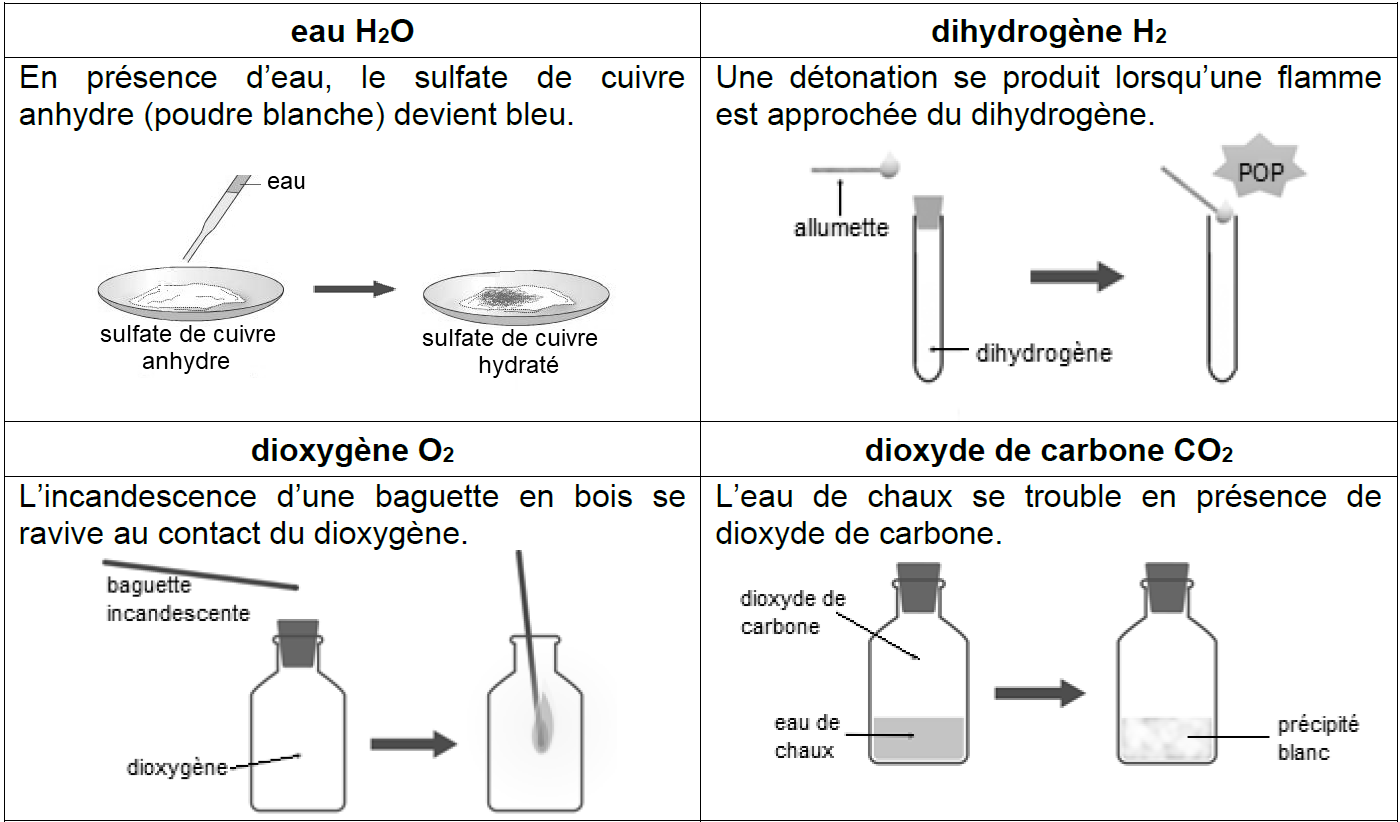
\includegraphics[scale=0.46]{Images/TP1/Tests_chimiques.png}
    \end{center}
\end{doc}

\begin{doc}{Pictogrammes de sécurité des produits utilisés lors du TP}
    \begin{minipage}{0.5\linewidth}
        
        \begin{center}
            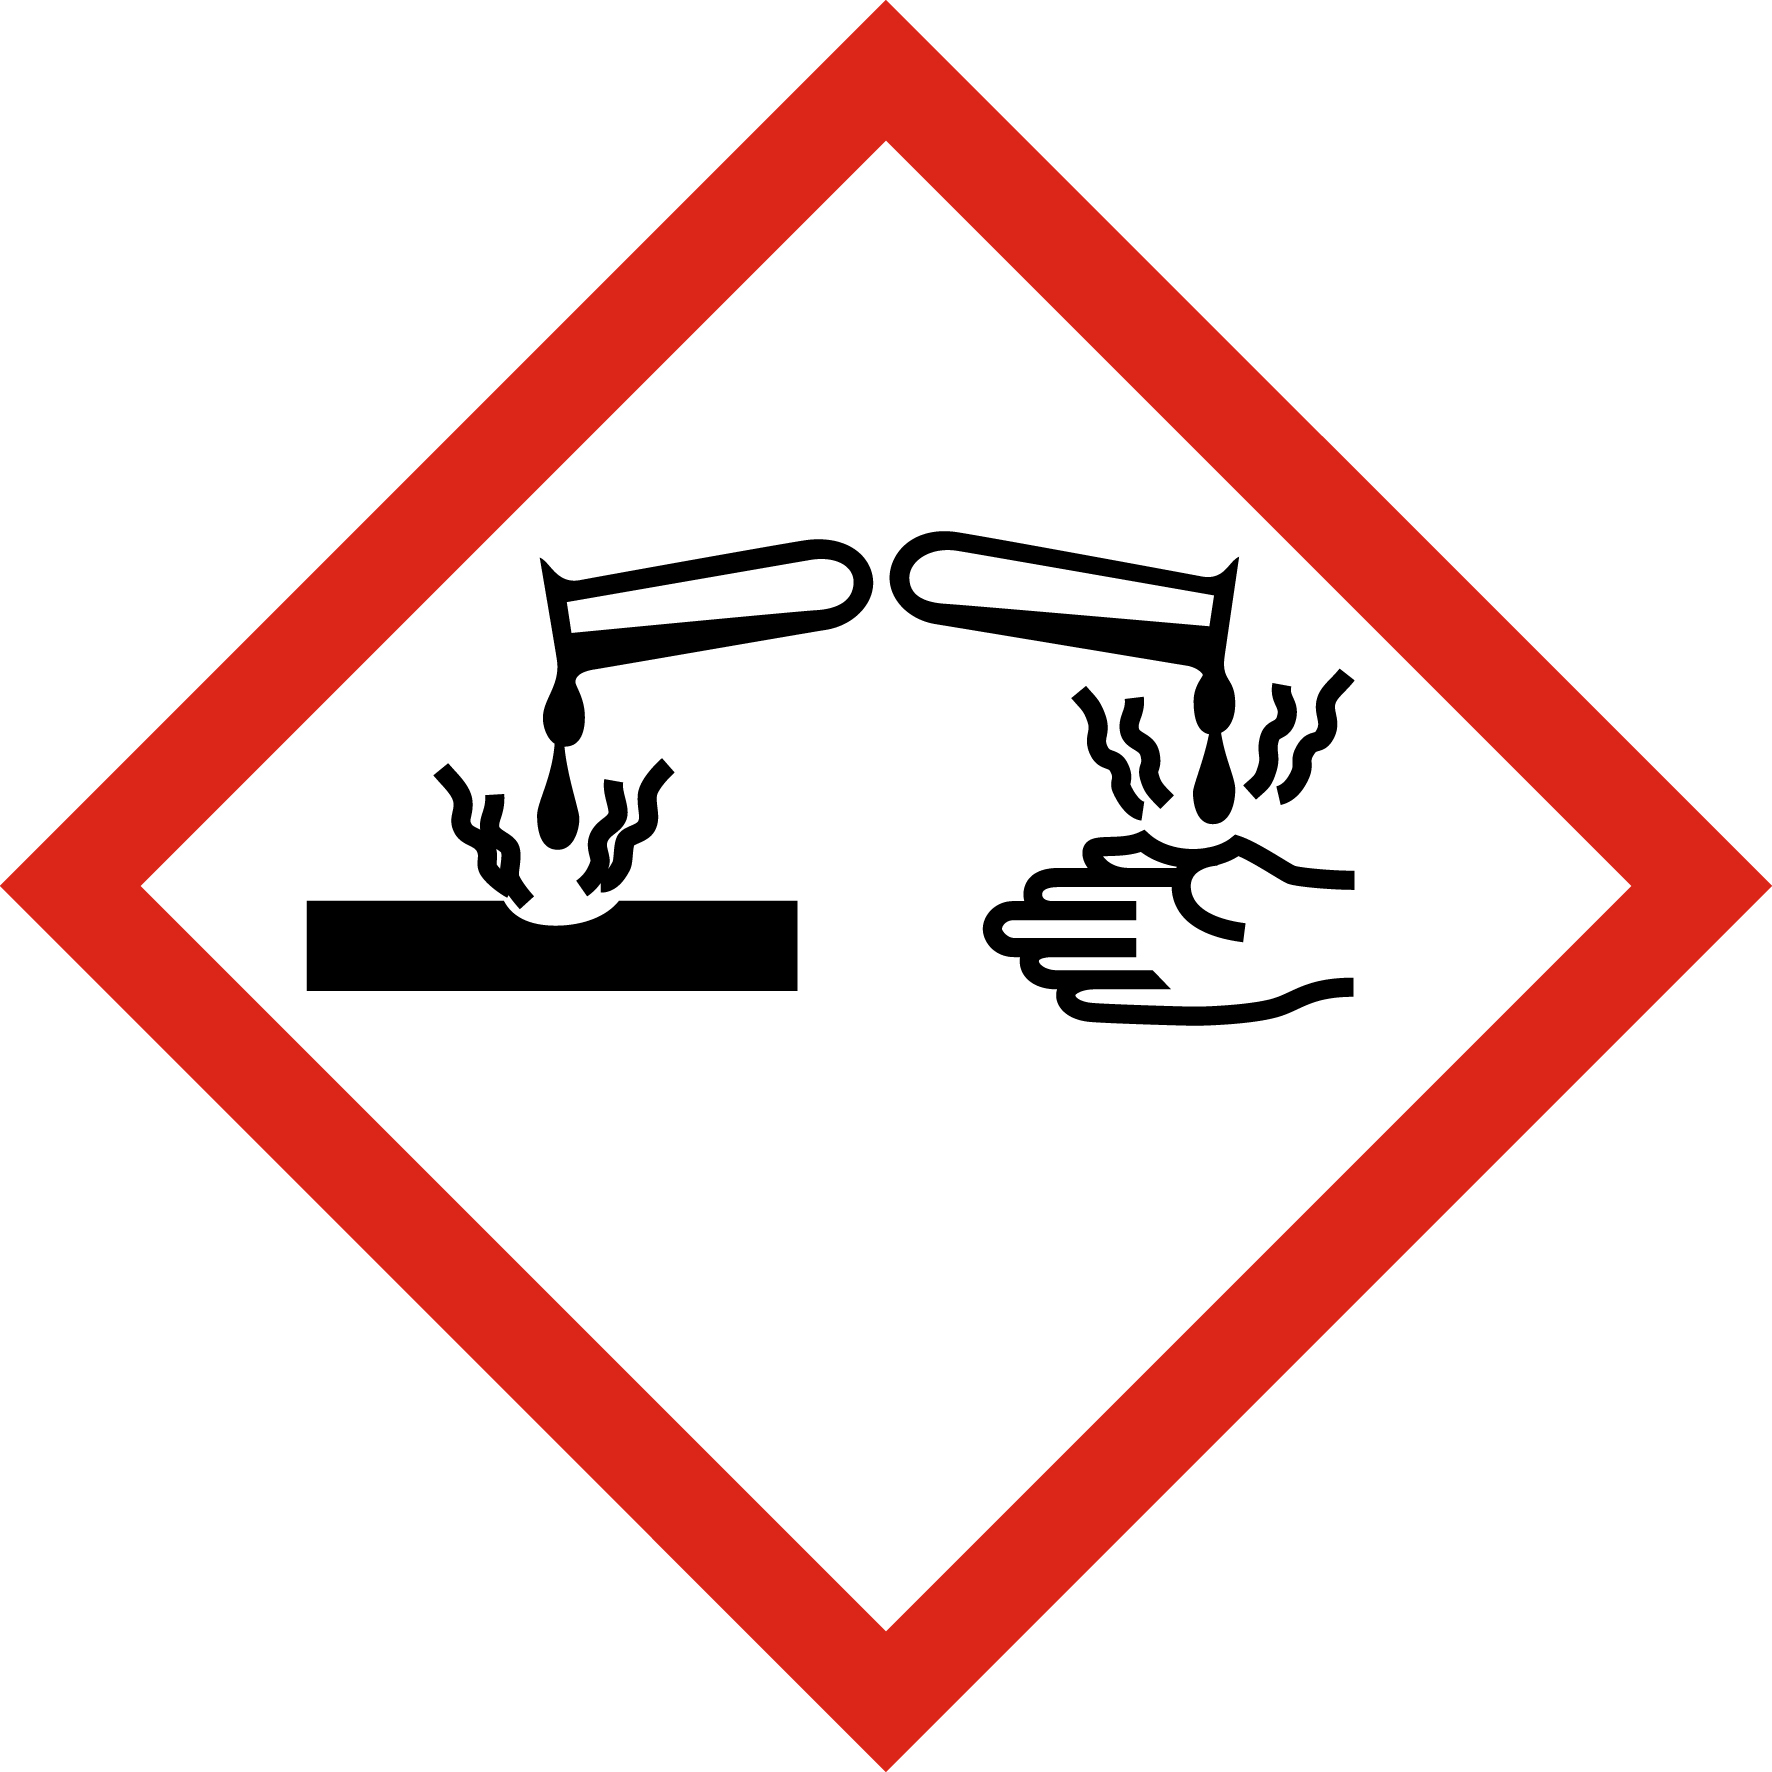
\includegraphics[scale=0.3]{Images/Fiche_Methode1/SGH05_Corrosion.jpg}
        \end{center}
        \begin{itemize}
            \item Solution d'acide chlorhydrique (\chemform{H^+_{(aq)}+Cl^-_{(aq)}})
            \item solution de chlorure de fer III (\chemform{Fe^{3+}_{(aq)}+3Cl^-_{(aq)}})
            \item eau oxygénée \chemform{H_2O_2}
        \end{itemize}
        
    \end{minipage}
    \begin{minipage}{0.5\linewidth}\vspace{-1.8cm}
    \begin{center}
        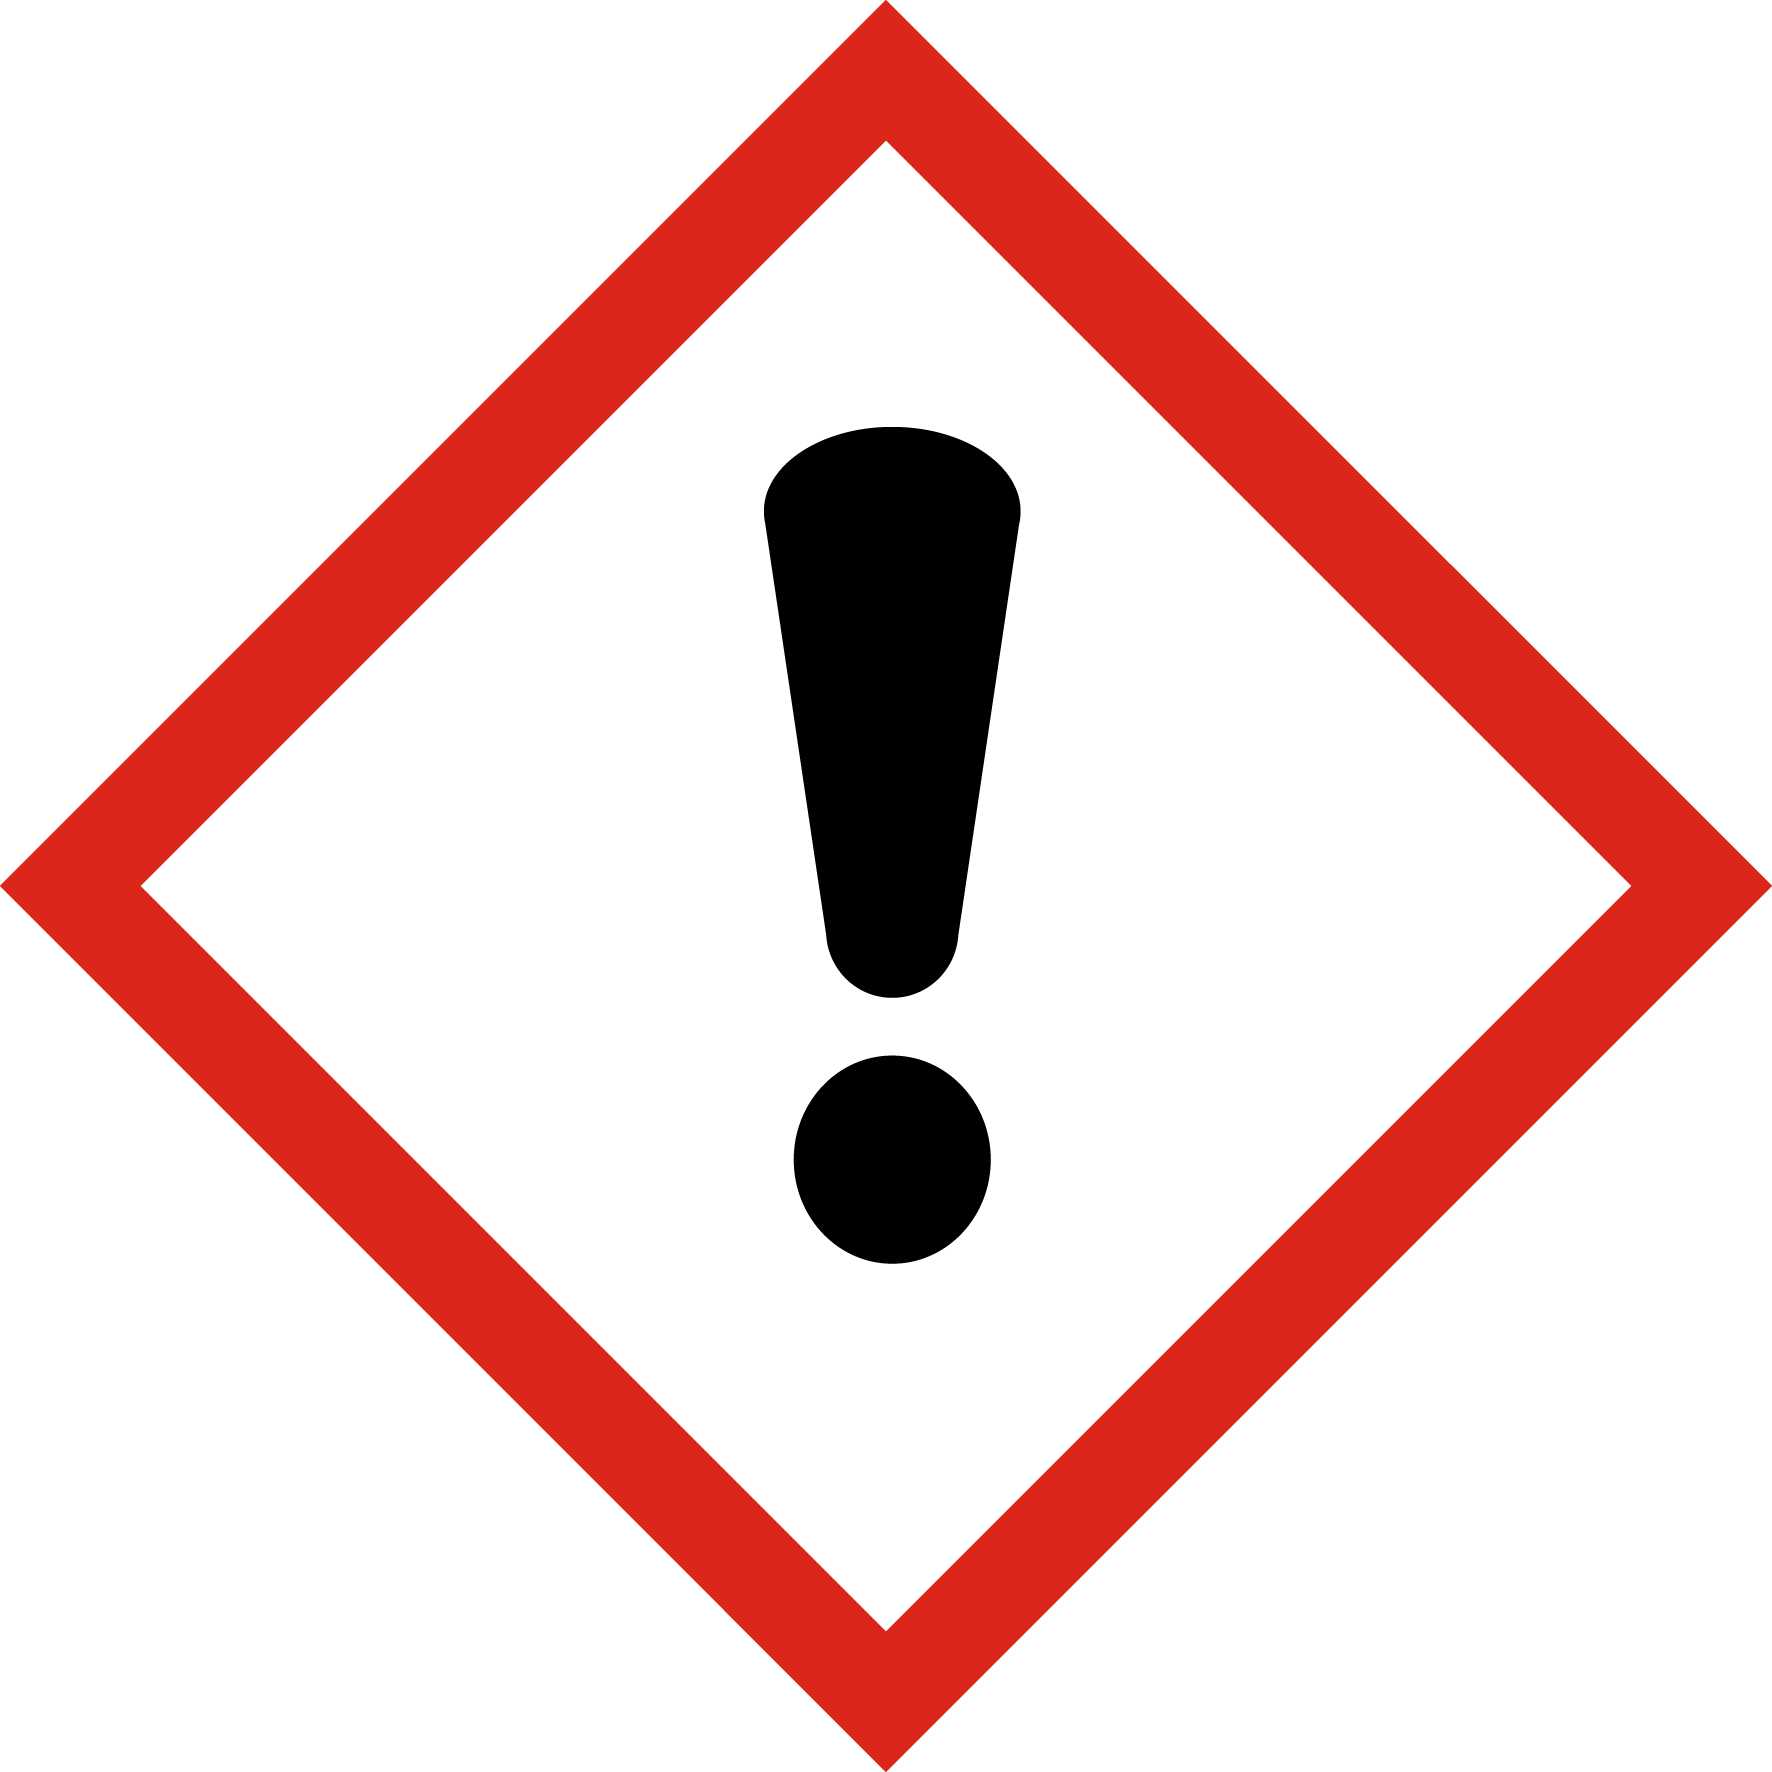
\includegraphics[scale=0.3]{Images/Fiche_Methode1/SGH07_PointExclamation.jpg}
    \end{center}
    \begin{itemize}
            \item eau de chaux (\chemform{Ca^{2+}_{(aq)}+HO^-_{(aq)}})
            \item sulfate de cuivre anhydride \chemform{CuSO_4(s)}
    \end{itemize}
    \end{minipage}
    \vspace{1cm}
    
    \begin{large}
        \ding{52}
    \end{large}Pour s'approprier les pictogrammes de sécurité : \url{https://learningapps.org/display?v=pz0yp6isn23} 
\end{doc}

\begin{doc}{Protocoles expérimentaux}
\begin{minipage}{\linewidth}
\begin{center}
    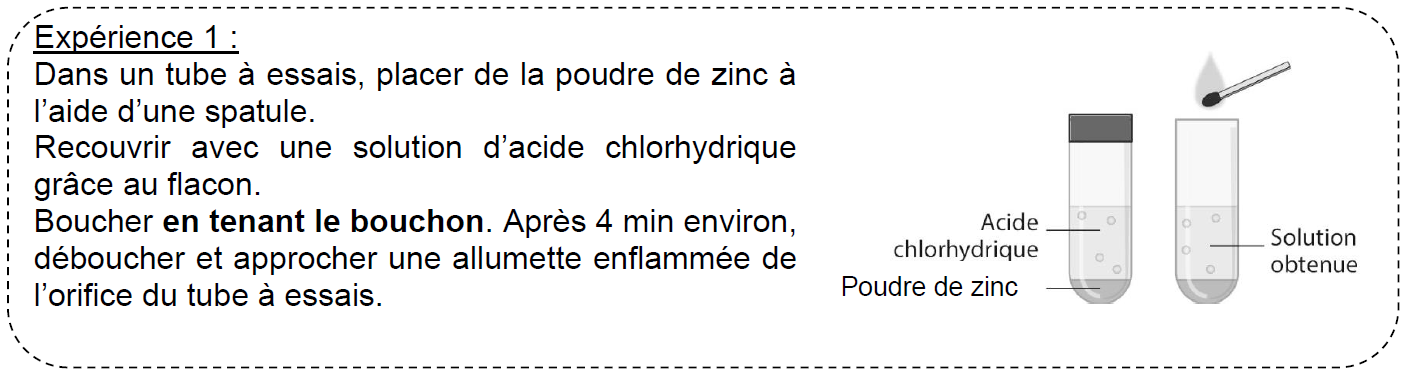
\includegraphics[scale=0.46]{Images/TP1/Exp_H2.png}
\end{center}
\end{minipage}
\begin{minipage}{\linewidth}
\begin{center}
    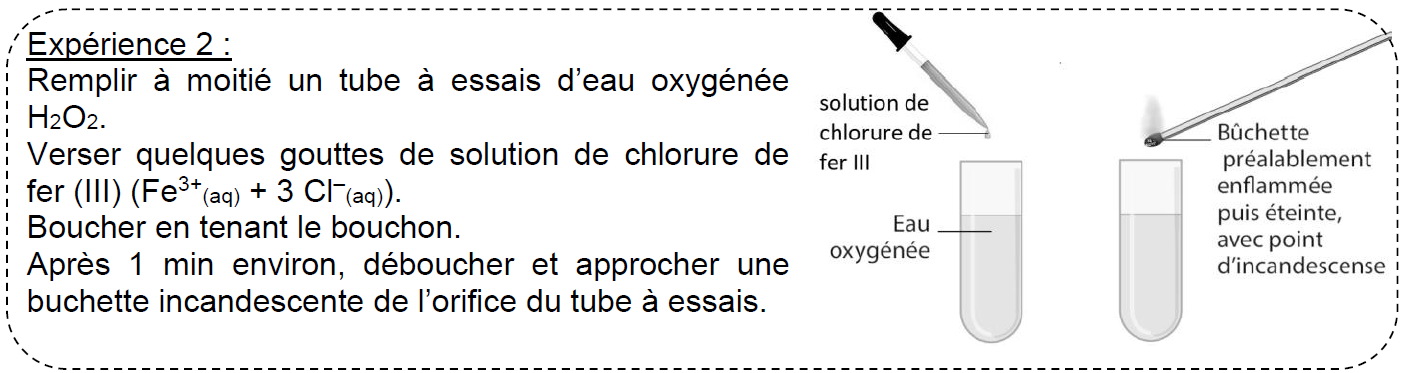
\includegraphics[scale=0.46]{Images/TP1/Exp_O2.png}
\end{center}
\end{minipage}
\begin{minipage}{\linewidth}
\begin{center}
    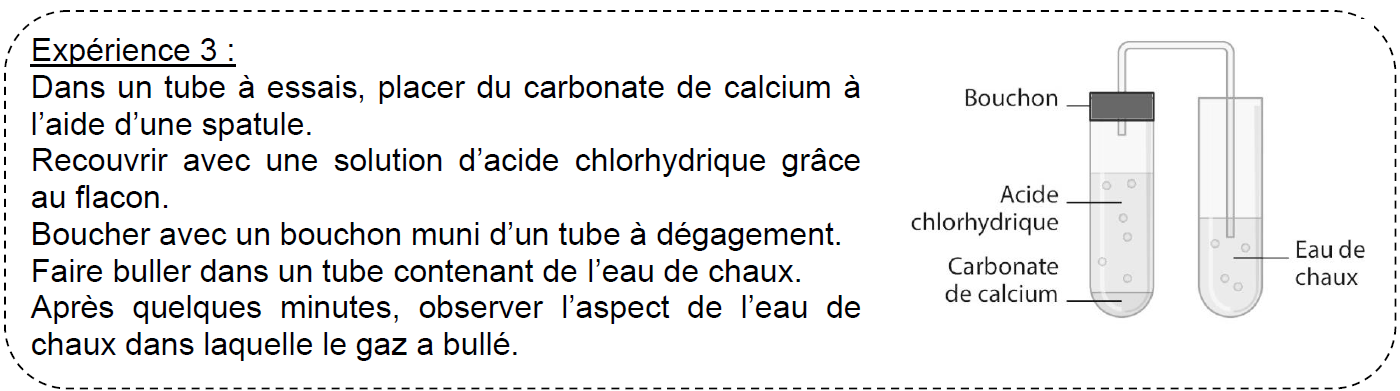
\includegraphics[scale=0.46]{Images/TP1/Exp_CO2.png}
\end{center}
\end{minipage}
\end{doc}

\begin{mdframed}[style=autreexo]
\textbf{\bsc{Liste du matériel}}
\begin{itemize}
    \item un flacon contenant de la poudre de zinc ;
    \item un flacon contenant une solution d’acide chlorhydrique ;
    \item un flacon contenant de l’eau oxygénée \chemform{H_2O_2};
    \item un flacon contenant une solution de chlorure de fer III ;
    \item un flacon contenant du carbonate de calcium en poudre ;
    \item une pissette d'éthanol à 95\% ;
    \item une solution de glycérol ;
    \item une spatule ;
    \item une boite d’allumettes ;
    \item une bûchette en bois ;
    \item des tubes à essais et leur support ;
    \item des bouchons pour tubes à essais ;
    \item un tube à dégagement et un bouchon pour tube à essais adapté ;
    \item une coupelle ;
    \item des béchers ;
    \item des pipettes simples ;
	\item des gants et des lunettes de protection.
 
\end{itemize}
\end{mdframed}

\newpage

\begin{Large}
    \textbf{\textcolor{red}{Travail à effectuer :}}
\end{Large}
\\
\begin{enumerate}
    \item Allumer votre ordinateur. Aller sur le site \url{https://learningapps.org/display?v=pz0yp6isn23} et effectuer l'activité.
    \item À l’aide du document 2, expliquer pourquoi il sera obligatoire de porter des gants, en plus de la blouse et des lunettes de protection, tout au long de l’activité.
    \item Réaliser les trois expériences du document 3 et noter vos observations expérimentales.
    \item À l’aide du document 1, identifier pour chacune des expériences du document 3 le gaz libéré.
    \item Compléter le tableau du document de cours avec vos observations
    \item On dispose de deux solutions : une d'éthanol commerciale et une de glycérol. Proposer un protocole permettant de déterminer si ces solutions contiennent de l'eau.
    \item Appeler le professeur pour valider ce protocole.
    \item Mettre en \oe uvre le protocole et noter vos observations expérimentales.
    \item La solution d'éthanol est-elle pure ? Que veut dire \og Solution d'éthanol à 95\% \fg ?
\end{enumerate}

\textit{Bonus pour les plus rapides : calculer la masse d'éthanol contenue dans la bouteille suivante : }

\begin{minipage}{0.5\textwidth}
\centering
    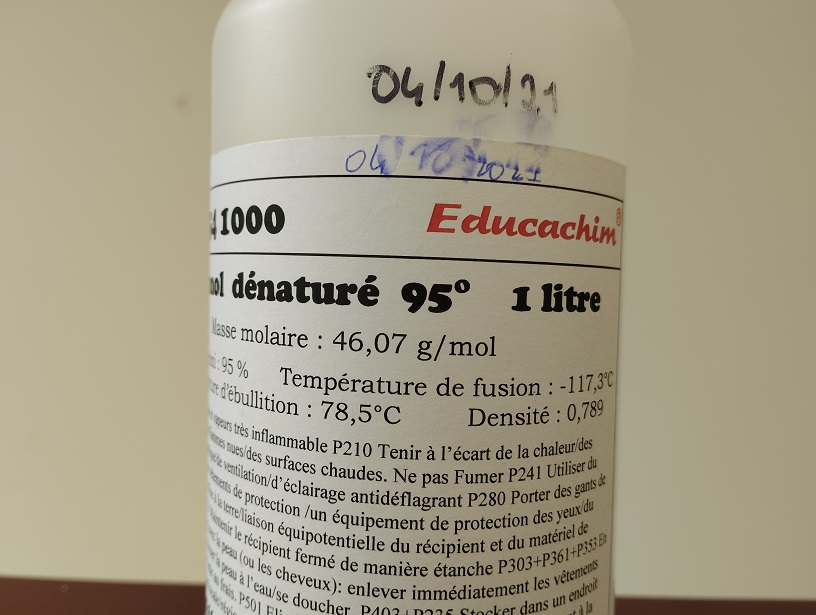
\includegraphics[scale=0.3]{Images/TP1/Bouteille_ethanol.jpg}
\end{minipage}
\begin{minipage}{0.5\textwidth}
\centering
    
\includegraphics[scale=0.3]{Images/TP1/qrcode_picto.png}
    \\
    QR-code pour les pictogrammes de sécurité.
\end{minipage}


  %%\newpage
%$ $
%\newpage

\renewcommand{\thesubsection}{\textcolor{red}{\Roman{section}.\arabic{subsection}}}
\renewcommand{\thesubsubsection}{\textcolor{red}{\Roman{section}.\arabic{subsection}.\alph{subsubsection}}}

\setcounter{section}{0}
\setcounter{document}{0}
\sndEnTeteTPDeux

\begin{center}
\begin{mdframed}[style=titr, leftmargin=60pt, rightmargin=60pt, innertopmargin=7pt, innerbottommargin=7pt, innerrightmargin=8pt, innerleftmargin=8pt]

\begin{center}
\large{\textbf{TP 2 : Mais qui a pollué la Seine ?}}
\end{center}

\end{mdframed}
\end{center}



\begin{tcolorbox}[colback=blue!5!white,colframe=blue!75!black,title=Objectifs de la séance :]
\begin{itemize}
    \item Mesurer une température de changement d'état,
    \item Réaliser une chromatographie sur couche mince,
\end{itemize}
\end{tcolorbox}

\begin{tcolorbox}[colback=orange!5!white,colframe=orange!75!black,title= Scénario:]
\og Le 5 août dernier, une compétition-test pré-JO de natation en eaux libres dans la Seine avait dû être annulée en raison de la pollution du fleuve.\fg 
\begin{flushright}
    \textit{Source : RadioFrance, le 16 août 2023}
\end{flushright}
\begin{large}
    \ding{43}
\end{large} Une grande usine est suspectée d’avoir déversé des milliers de litres de produits chimiques dans la Seine. Une équipe de scientifique a permis par évaporation d'isoler un solide blanc présent dans l'eau et un colorant. Vous avez pour mission de déterminer qui a déversé ces produits chimiques.
\end{tcolorbox}
\begin{center}
    \textbf{\textcolor{red}{Vous présenterez en fin de TP votre rapport d'enquêteur au professeur.}}
\end{center}

\section{Analyse d'une espèce solide}

\begin{doc}{Utilisation du banc Kofler}
Le banc Kofler est une plaque chauffante présentant un gradient de température, c’est à dire une augmentation progressive de la température de droite (température ambiante) à gauche (environ 250$\degreCelsius$-300$\degreCelsius$ selon les bancs). \textbf{Le banc Kofler permet de déterminer la température de fusion d’une espèce chimique}.
\begin{center}
    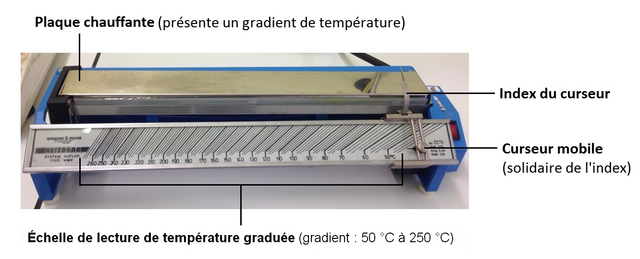
\includegraphics[scale=0.65]{Images/Chapitre_1/Banc_Kofler.png} 
\end{center}

Avant toute utilisation, le banc doit être étalonné (c’est-à-dire calibré). Voici les étapes d'utilisation du banc Kofler :
\begin{enumerate}
    \item \textbf{Etalonnage} \textit{(réalisé par le professeur)} : une très petite quantité de l’espèce étalon est déposée sur la partie froide du banc. On déplace ensuite cette quantité vers la partie chaude jusqu’à observer sa fusion. Le curseur de température est alors ajusté pour faire correspondre son index avec la température de l’étalon. Le banc doit ensuite être essuyé, pour enlever tous les résidus.
    \item \textbf{Mesure :} Comme lors de l’étalonnage, une petite quantité de l’espèce est déposée sur la partie froide du banc. On déplace ensuite cette quantité vers la partie chaude jusqu’à observer sa fusion. On lit à l’aide du curseur la température de fusion.
\end{enumerate}
Voici le lien d'une vidéo sur l'utilisation du banc : \url{https://ladigitale.dev/digiview/#/v/630614d1b4375}\\
\importantbox{Ne pas utiliser de gants lors de l'utilisation du banc Kofler !}
\end{doc}

\begin{doc}{Schéma des entreprises en bordure de la Seine}
\begin{center}
    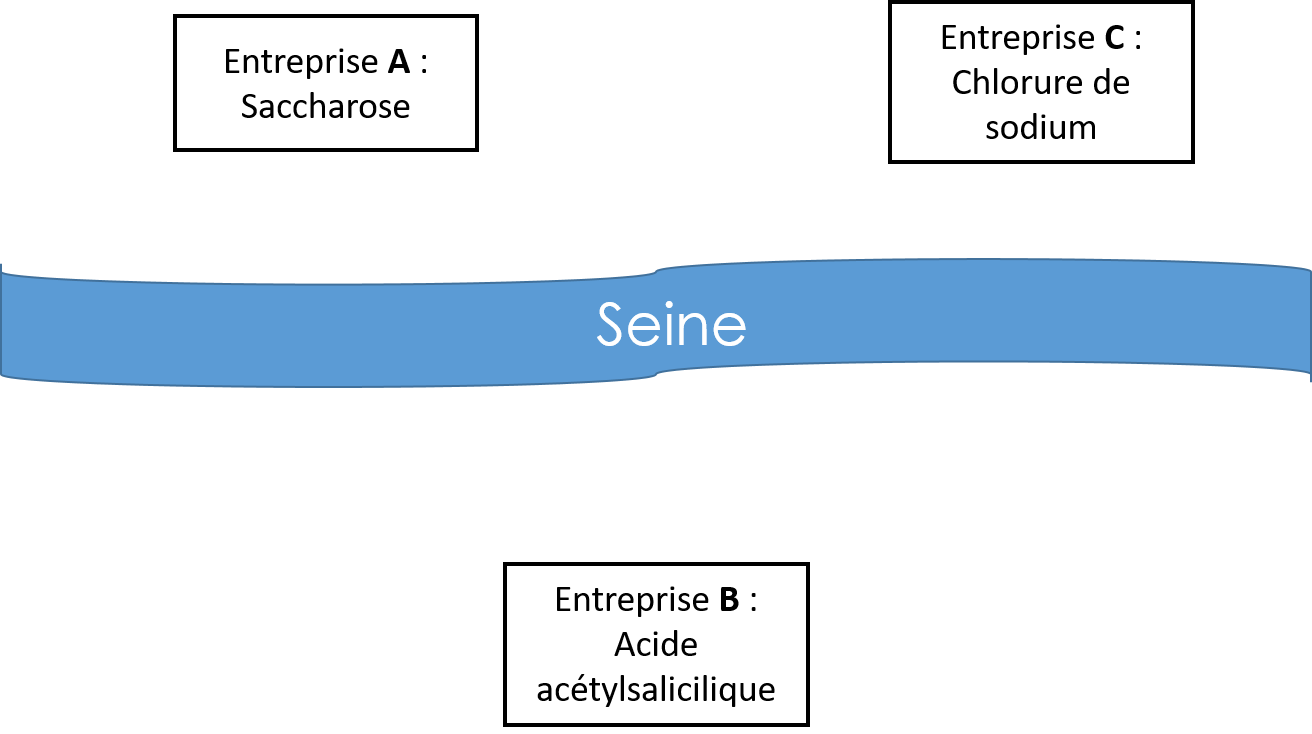
\includegraphics[scale=0.5]{Images/TP2/Entreprise.png}
\end{center}
\end{doc}
\newpage
\begin{doc}{Fiche technique des trois produits chimiques fabriqués par les entreprises}
\newline
    \begin{tabular}{|C{0.4}|C{0.1}|C{0.2}|C{0.2}|}
    \hline
     & Chlorure de sodium & Saccharose & Acide acétylsalycilique \\
    \hline
    Température de fusion $T_{f}$ \newline (en $\degreCelsius$) & 801 & 185,5 & 135 \\
    \hline
    Température d'ébullition $T_{eb}$ \newline (en $\degreCelsius$) & 1465 & Décomposition & Se décompose à 140 $\degreCelsius$ \\
    \hline
    Masse volumique (en g.cm$^{-3}$) & 2,16 & 1,59 & 1,4 \\
    \hline
    \end{tabular}
\end{doc}

\textbf{Vous souhaitez déterminer l’entreprise d’où provient la poudre retrouvée sur la victime pour en déduire ainsi le lieu du crime.}\\
A l’aide des documents :
\begin{enumerate}
    \item Trouver et rédiger le protocole à mettre en place
    \item Réaliser l’expérience
    \item Déterminer le lieu du crime en justifiant,
    \item \textit{(Bonus)} Proposer une autre technique qui aurait pu permettre de déterminer le lieu du crime
\end{enumerate}

\section{Analyse d'un colorant}
Maintenant que vous avez découvert le lieu du crime, les enquêteurs penchent sur deux suspects : le Professeur Violet qui utilise les colorants E102 et E131 et le Docteur Orchidée qui utilise le colorant E133.\\

\begin{doc}{Mettre en place une Chromatographie sur Couche Mince (CCM)}
Protocole expérimental :
    \begin{itemize}
        \item Introduire l’éluant (eau + éthanol) dans la cuve à chromatographie (sur environ 0,5 cm de hauteur). Fermer la cuve avec son couvercle pour la saturer en vapeurs d’éluant.
        \item Tracer, au crayon, sur le papier filtre la ligne de dépôt à 1,5 cm du bord inférieur. Placer, en les espaçant d’au moins 1 cm, une marque par dépôt à effectuer (ici 4 dépôts, \textbf{notez les sur le papier filtre !}),
        \item Déposer les échantillons à analyser à l’aide d’un tube capillaire. Un dépôt pour le feutre, un dépôt pour la tâche, un dépôt pour l’encre.
        \item Introduire la plaque dans la cuve (attention, la ligne de dépôt et les échantillons ne doivent pas être immergés dans l’éluant !) 
        \item Retirer la plaque à chromatographie de la cuve lorsque l’éluant a migré jusqu’à atteindre 1 cm du bord supérieur. Tracer au crayon le front de solvant.
    \end{itemize}
Une animation pour réaliser une CCM est disponible à cette adresse \url{https://ladigitale.dev/digiplay/#/v/63061cea42993} 
\end{doc}
%\qrcode{https://ladigitale.dev/digiplay/#/v/63061cea42993}
\begin{doc}{Analyse comparative d'un ou plusieurs chromatogrammes}
\begin{wrapfigure}{r}{0.4\textwidth}
\vspace{-1cm}
    \centering
      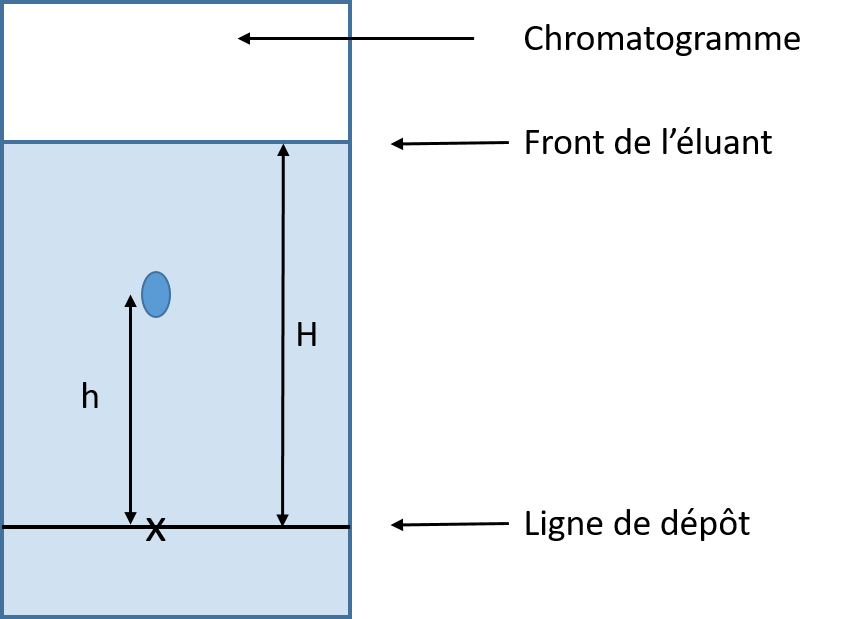
\includegraphics[width=0.4\textwidth]{Images/TP2/Chromatogramme.png}
  \end{wrapfigure}
    Le rapport frontal (noté $R_f$) se calcule à l'aide de la formule suivante :
\begin{equation*}
    R_f = \frac{h}{H}
\end{equation*}
avec $h$ la distance parcourue par l'espèce chimique, $H$ la distance parcourue par le front de l'éluant.\\
\textbf{Si deux espèces chimiques ont le même rapport frontal, alors elles sont identiques.}

\end{doc}



\begin{mdframed}[style=autreexo]
\textbf{\bsc{Liste du matériel}}
\begin{itemize}
    \item tube capillaire,
    \item flacon de colorant E133 ;
    \item flacon de colorant E102 ;
    \item flacon de colorant E131 ;
    \item papier filtre ;
    \item cuve chromatographique ;
\end{itemize}
\end{mdframed}
A l’aide des documents :
\begin{enumerate}
    \item À l’aide d’un schéma, présenter les résultats de la CCM,
    \item Interpréter les résultats de la CCM,
    \item Déterminer le coupable.
\end{enumerate}
  %%\newpage
%$ $
%\newpage

\renewcommand{\thesubsection}{\textcolor{red}{\Roman{section}.\arabic{subsection}}}
\renewcommand{\thesubsubsection}{\textcolor{red}{\Roman{section}.\arabic{subsection}.\alph{subsubsection}}}

\setcounter{section}{0}
\setcounter{document}{0}
\sndEnTeteTPTrois

\begin{center}
\begin{mdframed}[style=titr, leftmargin=60pt, rightmargin=60pt, innertopmargin=7pt, innerbottommargin=7pt, innerrightmargin=8pt, innerleftmargin=8pt]

\begin{center}
\large{\textbf{TP 3 : Détermination de la composition d'un mélange : l'alcool pharmaceutique}}
\end{center}

\end{mdframed}
\end{center}



\begin{tcolorbox}[colback=blue!5!white,colframe=blue!75!black,title=Objectifs de la séance :]
Mesurer des volumes et des masses pour estimer la composition de mélanges.
\end{tcolorbox}

\begin{tcolorbox}[colback=orange!5!white,colframe=orange!75!black,title= Scénario:]
Un pharmacien vend de l’alcool pharmaceutique (mélange eau-éthanol), qui sert de désinfectant notamment pour le matériel médical. L’étiquette d’un flacon d’alcool pharmaceutique porte la mention de sa composition. Le pharmacien aimerait s’assurer que cette indication est correcte.
\end{tcolorbox}

\section{Documents mis à disposition}

\begin{multicols}{2}
    \begin{doc}{Flacon d'alcool pharmaceutique}
\begin{center}
    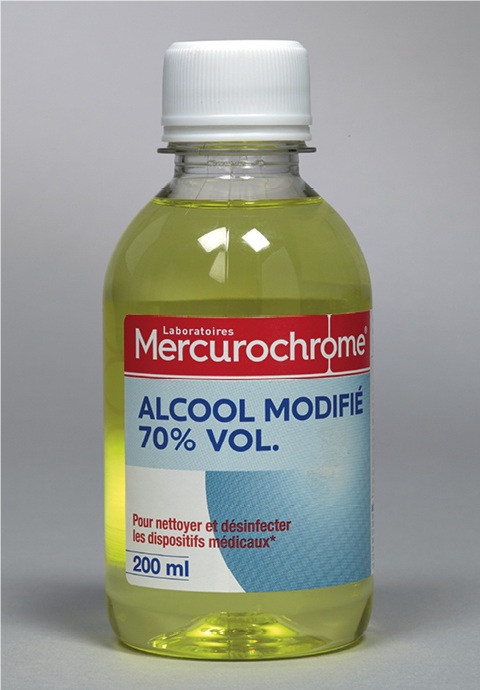
\includegraphics[scale=0.81]{Images/TP3/Alcool_pharma.png}
\end{center}
\end{doc}
\begin{doc}{Variation de la masse volumique d’un mélange eau-éthanol en fonction du pourcentage volumique en éthanol}
\vspace{-1cm}
\begin{center}
    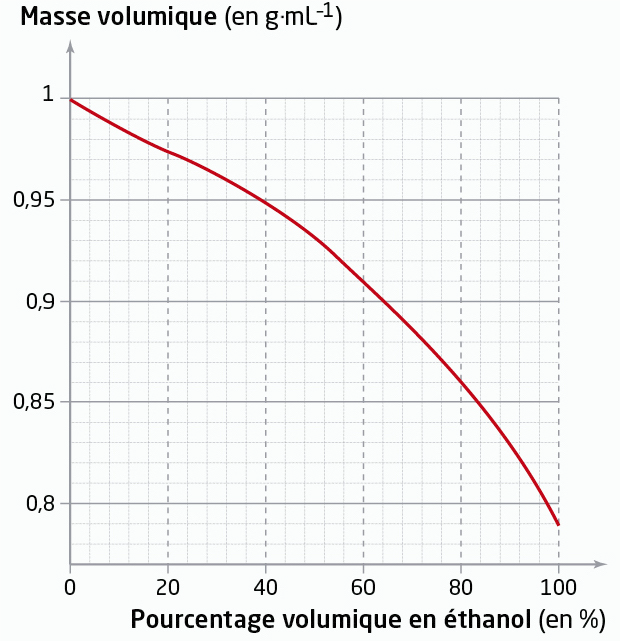
\includegraphics[scale=0.75]{Images/TP3/Masse_vol_ethanol.png}
\end{center}
\end{doc}

\end{multicols}

\newpage

\begin{mdframed}[style=autreexo]
\textbf{\bsc{Liste du matériel}}
\begin{itemize}
    \item un flacon contenant de l'alcool pharmaceutique
    \item une balance
    \item une éprouvette graduée de 10mL
    \item une fiole jaugée de 25mL
    \item une pissette en plastique
    \item un bécher de 25mL 
\end{itemize}
\end{mdframed}


\section{Travail à effectuer}

\question{À l’aide du document 2, déterminer la masse volumique de l’éthanol pur, ainsi que la masse volumique de l’eau.}{Par lecture graphique, on lit $\rho_{eau}=1$~g.mL$^{-1}$ lorsque le pourcentage volumique en éthanol est égal à 0\% et $\rho_{ethanol}=0.79$~g.mL$^{-1}$ lorsque le pourcentage volumique en éthanol est égal à 100\%.}{0}

\question{Proposer un protocole permettant de déterminer expérimentalement la masse volumique de l’alcool pharmaceutique vendu par le pharmacien.}{On pèse la verrerie qu'on va utiliser (bécher, fiole jaugée ou éprouvette graduée). On tare la balance (ou on note la masse de la verrerie pour la soustraire par la suite). On verse un volume V d'alcool pharmaceutique dans la verrerie en s'aidant des traits de graduation de la verrerie. On vérifie que le bas du ménisque coïncide bien avec la graduation. On note le volume versé $V$. On pèse ensuite l'ensemble \{verrerie+alcool\} pour en déduire la masse d'alcool versé.}{0}

\question{Appeler le porfesseur pour valider votre protocole expérimental.}{}{0}

\question{Mettre en \oe uvre le protocole précédent et déterminer la masse volumique de l’alcool pharmaceutique vendu par le pharmacien.}{On pèse l'éprouvette graduée à vide, on remplit d'un certain volume d'alcool pharmaceutique $V$ et on pèse l'ensemble. On en déduit la masse volumique $\rho=\frac{m_{verrerie+eau/ethanol}-m_{verrerie}}{V}$
. On laisse ici le choix de la verrerie, le TP suivant permettra d'appréhender la précision des différents types de verrerie. Mais pour une mesure précise, il faut choisir ici une fiole jaugée.}{0}

\question{La législation autorise un écart de $\pm~2\%$.VOL sur la proportion volumique d'éthanol contenue dans ce produit. Déterminer si l’indication portée sur le flacon d’alcool pharmaceutique vendu est conforme.}{La mesure doit être conforme à la valeur indiquée. Si l'écart entre la mesure et la valeur indiquée est supérieur à 2\%, on peut mettre en cause :
\begin{itemize}
    \item le choix de la verrerie dans le protocole : effectivement, si le choix s'est porté sur le bécher, le volume lu est peu précis (5\% sur la valeur lue au moins),
    \item la quantité réelle d'éthanol contenue : l'éthanol étant volatil, une petite quantité a pu s'évaporer du flacon modifiant la masse volumique du mélange.
\end{itemize}}{0}

\question{L’alcool pharmaceutique vendu par le pharmacien a été préparé en utilisant 75 mL d’eau. Calculer le volume d’éthanol qu’il a fallu ajouter pour fabriquer cet alcool.}{On sait que la proportion volumique en éthanol vaut $x_V=\frac{V_{ethanol}}{V_tot}=70$\%. Comme $V_{tot}=V_{ethanol}+V_{eau}$, on en déduit : 
\begin{align*}
    \frac{V_{ethanol}}{V_{ethanol}+V_{eau}} &= 0,70 \\
    V_{ethanol} &= 0,70\times (V_{ethanol}+V_{eau}) \\
    V_{ethanol}\times (1-0,70) &= V_{eau} \\
    V_{ethanol}  &= \frac{V_{eau}}{1-0,70} = \frac{75~\text{mL}}{1-0,70}=250~\text{mL}
\end{align*}}{0}
  %\modeCorrection

\nomPrenomClasse

\begin{center}
\begin{Large}
    
    Interrogation de cours : Corps purs et mélanges au quotidien (10min)
\end{Large}
\end{center}
\vspace{1cm}


\question{Citer un test chimique pour reconnaitre la présence de dioxyde de carbone \chemform{CO_2}.}{Le \chemform{CO_2} réagit avec l'eaux de chaux pour former un précipité blanc. L'eau de chaux se trouble donc en présence de \chemform{CO_2}.}{2}

\question{L'acétone est miscible avec l'eau. Que cela veut-il dire ? Citer deux espèces chimiques non miscibles.}{Le mélange eau-acétone est homogène. L'huile et l'eau ne sont pas miscibles. On pourrait également citer le graphite avec de l'huile par exemple.}{2}

\question{Donner la formule de la densité d'une espèce chimique. Donner la signification et l'unité de chaque grandeur physique introduite (y compris la densité).}{La densité $d$ d'une espèce chimique est donnée par la formule :
\begin{equation*}
    d = \frac{\rho_{\text{espèce}}}{\rho_{eau}}
\end{equation*} avec $\rho$ la masse volumique (en g.cm$^{-3}$ ou g.L$^{-1}$). La densité s'exprime sans unité.}{3}
\\
\newline
\newline
  %\renewcommand{\thesubsection}{\textcolor{red}{\Roman{section}.\arabic{subsection}}}
\renewcommand{\thesubsubsection}{\textcolor{red}{\Roman{section}.\arabic{subsection}.\alph{subsubsection}}}

\setcounter{section}{0}
\setcounter{document}{0}
\sndEnTeteActUn

\begin{center}
\begin{mdframed}[style=titr, leftmargin=60pt, rightmargin=60pt, innertopmargin=7pt, innerbottommargin=7pt, innerrightmargin=8pt, innerleftmargin=8pt]

\begin{center}
\large{\textbf{Activité 1 : Composition d'un mélange eau-huile}}
\end{center}

\end{mdframed}
\end{center}
\begin{Large}{\textbf{Q : Quelle est la proportion volumique et massique de l'huile et de l'eau présent dans l'éprouvette graduée sur le bureau du professeur ?}} \end{Large} 
\begin{mdframed}[style=autreexo]
\textbf{\bsc{Consignes :}}
\begin{itemize}
    \item Lever la main si vous souhaitez vous déplacer,
    \item Lever la main si vous souhaitez un indice,
    \item Vous pouvez travailler en binôme \textbf{\underline{uniquement}} avec votre voisin de table,
    \item Vous pouvez rendre le travail à la fin de l'heure si vous améliorer votre note d'interrogation.
   
\end{itemize}
\end{mdframed}

\begin{doc}{Lecture d'un volume sur la verrerie}

\begin{wrapfigure}{r}{0.3\textwidth}
\vspace{-2cm}
    \centering
      \includegraphics[width=0.27\textwidth]{Images/Activite/Chap1/Lecture_Verrerie.png}
  \end{wrapfigure}
  Lorsqu'on verse un liquide dans une pièce de verrerie (éprouvette, tube à essai, etc), l se forme un ménisque qui va perturber la mesure du volume sur cette verrerie. Pour lire le volume occupé par un liquide, il faut positionner son \oe il sur le bas du ménisque.%En 1775, Antoine Lavoisier réalise une expérience qui lui permet de déterminer la composition de l’air.
%Son expérience est résumée dans la vidéo suivante : \url{https://ladigitale.dev/digiplay/#/v/6305f2f7b8fd4}.\\
%D’après Lavoisier, l’air est constitué de deux gaz : le dioxygène et le diazote. Le volume du gaz initialement
%présent dans la cloche est de 0,80 L d’air. À la fin de l’expérience, le volume du gaz qui n’a pas réagi avec le
%mercure (c’est-à-dire le diazote) est de 0,66 L.}
\end{doc}

\begin{doc}{Proportion volumique ou massique d’une espèce dans un mélange}
Pour décrire la composition d’un mélange, on indique la proportion (ou le pourcentage) de chaque espèce chimique constituant le mélange. On peut choisir d’utiliser la proportion massique notée $x_m$, ou la proportion volumique notée $x_V$ :
\begin{align*}
    x_m &= \frac{m_{\text{espèce}}}{m_{\text{totale}}} & x_V & = \frac{V_{\text{espèce}}}{V_{\text{totale}}}\\
\end{align*}
Ces deux grandeurs s'expriment en général en \%.
\end{doc}

\begin{doc}{Données utiles}
La masse volumique de l'huile est :
\begin{equation*}
    \rho_{huile} = 0,92 \text{~g.cm$^{-3}$}
    \end{equation*}
\end{doc}

  %\renewcommand{\thesubsection}{\textcolor{red}{\Roman{section}.\arabic{subsection}}}
\renewcommand{\thesubsubsection}{\textcolor{red}{\Roman{section}.\arabic{subsection}.\alph{subsubsection}}}

\setcounter{section}{0}
\setcounter{document}{0}
\sndEnTeteActUn

\begin{center}
\begin{mdframed}[style=titr, leftmargin=60pt, rightmargin=60pt, innertopmargin=7pt, innerbottommargin=7pt, innerrightmargin=8pt, innerleftmargin=8pt]

\begin{center}
\large{\textbf{Activité 1 : Composition d'un mélange eau-huile - \textbf{Correction}}}
\end{center}

\end{mdframed}
\end{center}
\begin{Large}{\textbf{Q : Quelle est la proportion volumique et massique de l'huile et de l'eau présent dans l'éprouvette graduée sur le bureau du professeur ?}} \end{Large}
\newline

\`{A} la lecture sur l'éprouvette graduée, on lisait :
\begin{enumerate}
    \item $V_{huile}=15$~mL,
    \item $V_{eau}=30$~mL,
    \item $V_{Tot}= 45$~mL $=V_{huile}+V_{eau}$
\end{enumerate}

\section{Calcul de la proportion volumique de l'huile et de l'eau}
On en déduit directement la proportion volumique pour chaque espèce :
\begin{enumerate}
    \item $x_V(huile)=\frac{V_{huile}}{V_{Tot}}=\frac{15}{45}=33\%$
    \item $x_V(eau)=\frac{V_{eau}}{V_{Tot}}=\frac{30}{45}=67\%$
    \item \textcolor{red}{On vérifie bien que $x_V(huile)+x_V(eau)=100\%$}
\end{enumerate}

\section{Calcul de la proportion massique de l'huile et de l'eau}
Maintenant pour calculer la proportion massique de chaque espèce chimique, on doit d'abord calculer la masse de chaque espèce chimique. \\

\textbf{\underline{D'après le cours}}, la relation qui lie la masse et le volume est celle de la masse volumique à savoir :
\begin{equation*}
    \rho_{\text{espèce}} = \frac{m_{\text{(espèce)}}}{V_{\text{espèce}}}
\end{equation*}

On en déduit donc :
\begin{enumerate}
    \item $m_{\text{eau}}=\rho_{\text{eau}}\times V_{\text{eau}}=1,0~\text{g/mL}\times 30~\text{mL}=30$~g. \textcolor{red}{On ne garde que deux chiffres significatifs au résultat},
    \item $m_{\text{huile}}=\rho_{\text{huile}}\times V_{\text{eau}}=0,92~\text{g/mL}\times 15~\text{mL}=14$~g. \textcolor{red}{On ne garde que deux chiffres significatifs au résultat}
    \item $m_{Tot}=m_{\text{huile}}+m_{\text{eau}}=44$~g.
\end{enumerate}

On en déduit donc d'après le Document 2 la proportion massique des deux espèces :
\begin{align*}
    x_m(eau)&=\frac{m_{\text{eau}}}{m_{Tot}}=\frac{30}{44}=68\% & x_m(huile)&=\frac{m_{\text{eau}}}{m_{Tot}}=\frac{14}{44}=32\% 
\end{align*}
\textcolor{red}{On vérifie bien que $x_m(huile)+x_m(eau)=100\%$}
  %\renewcommand{\thesubsection}{\textcolor{red}{\Roman{section}.\arabic{subsection}}}
\renewcommand{\thesubsubsection}{\textcolor{red}{\Roman{section}.\arabic{subsection}.\alph{subsubsection}}}

\setcounter{section}{0}
\setcounter{document}{0}
\sndEnTeteDMUn

\begin{center}
\begin{mdframed}[style=titr, leftmargin=60pt, rightmargin=60pt, innertopmargin=7pt, innerbottommargin=7pt, innerrightmargin=8pt, innerleftmargin=8pt]

\begin{center}
\large{\textbf{Devoir maison 1 : la composition de l'air}}
\end{center}

\end{mdframed}
\end{center}

\begin{wrapfigure}{r}{0.3\textwidth}
\vspace{-1cm}
    \centering
      \includegraphics[width=0.3\textwidth]{Images/Activite/Chap1/Lavoisier.PNG}
  \end{wrapfigure}
Antoine Laurent Lavoisier (1743-1794) est considéré comme le père de la chimie moderne. Avec ses multiples expériences sur l’air, le dioxygène, ou le dioxyde de carbone, il montre que la matière est
constituée d’espèces chimiques (même s’il n’emploie pas ce terme), et non de quatre éléments (feu, terre, eau et air) comme les anciens chimistes
l’admettaient.\\
\newline

\begin{doc}{Lecture d'un volume sur la verrerie}
\begin{wrapfigure}{r}{0.2\textwidth}
\vspace{-1cm}
    \centering
      \includegraphics[width=0.2\textwidth]{Images/DM/Qr_code_Lavoisier.png}
  \end{wrapfigure}
En 1775, Antoine Lavoisier réalise une expérience qui lui permet de déterminer la composition de l’air.
Son expérience est résumée dans la vidéo suivante : \url{https://ladigitale.dev/digiplay/#/v/6305f2f7b8fd4}.\\
D’après Lavoisier, l’air est constitué de deux gaz : le dioxygène et le diazote. Le volume du gaz initialement
présent dans la cloche est de 0,80 L d’air. À la fin de l’expérience, le volume du gaz qui n’a pas réagi avec le mercure (c’est-à-dire le diazote) est de 0,66 L.
\end{doc}

\begin{doc}{Proportion volumique ou massique d’une espèce dans un mélange}
Pour décrire la composition d’un mélange, on indique la proportion (ou le pourcentage) de chaque espèce chimique constituant le mélange. On peut choisir d’utiliser la proportion massique notée $x_m$, ou la proportion volumique notée $x_V$ :
\begin{align*}
    x_m &= \frac{m_{\text{espèce}}}{m_{\text{totale}}} & x_V & = \frac{V_{\text{espèce}}}{V_{\text{totale}}}\\
\end{align*}
Ces deux grandeurs s'expriment en général en \%.
\end{doc}

\begin{doc}{Données utiles}
On donne les informations suivantes à pression atmosphérique :
\begin{itemize}
    \item 1 mL de dioxygène a une masse $m_{O_2}
=1,354$~mg à $15\degreCelsius$,
    \item 1 mL de diazote a une masse $m_{N_2}
=1,185$~mg à $15\degreCelsius$,
    \item 1 mL d’air ambiant a une masse $m_{air}=1,225$~mg à $15\degreCelsius$.
\end{itemize}
\end{doc}

\newpage

\question{Résumer en quelques lignes l’expérience de Lavoisier}{Lavoisier fait chauffer un récipient (un matras) rempli de mercure qui est relié à une cloche remplie d'air placée dans une bassine d'eau servant à mesurer le volume d'air présent dans la cloche. Au deuxième jour d'expérience, le mercure réagit avec le dioxygène présent de la cloche formant un précipité d'oxyde de mercure \chemform{HgO}. Le volume qu'occupe le gaz dans la cloche a donc diminué. Lavoisier place une souris dans la cloche et celle-ci meurt. Il en déduit que c'est le dioxygène qui a régit avec le mercure et nomme l'autre gaz \og azote \fg. Par la lecture du volume, Lavoisier peut en déduire la proportion de chaque espèce présente dans l'air.}{4}
\\
\question{Déterminer si l’air est un corps pur, un mélange homogène ou un mélange hétérogène. Justifier.}{D'après le document 1, l'air est constitué d'au moins deux gaz différents : le dioxygène \chemform{O_2}, le diazote \chemform{N_2}. Il s'agit donc d'un mélange (ici gazeux). On ne distingue pas les deux gaz à l'\oe il nu. L'air est donc un mélange homogène.}{2}
\\
\question{Calculer la proportion volumique de diazote dans l’air obtenue d'après l'expérience de Lavoisier.}{D'après le document 1, le volume de diazote n'ayant pas réagi avec le mercure vaut $V_{N_2}=0,66$~L. Le volume total de gaz initialement présent dans la cloche était de $V_{tot}=0,80$~L. On en déduit la proportion volumique de \chemform{N_2} d'après la formule donnée par le document 3 : \begin{equation*}
    x_{V}(N_2)=\frac{V_{N_2}}{V_{tot}}=\frac{0,66}{0,80} = 0,83 = 83\%
\end{equation*}}{2}
\\
\question{Déduire de la question précédente le volume initial du dioxygène. Quelle était la masse initiale $m_{O_2}(ini)$ de dioxygène dans l'expérience de Lavoisier ?}{On déduit de la proportion volumique de diazote de la question précédente la proportion volumique de dioxygène :
\begin{equation*}
    x_V(O_2) =1-x_V(N_2) = 17\%
\end{equation*}
On en déduit le volume initial de dioxygène par rapport au volume total de la cloche $V_{tot}=0.80$~L :
\begin{equation*}
    V(O_2)=x_V(O_2)\times V_{tot}=0,17\times 0,80 = 0,14~\text{L} = 140~\text{mL}
\end{equation*}
Remarque : ce résultat est bien sur cohérent avec les données du document 1 : $V(O_2)=V_{tot}-V(N_2)=0,80-0,66=0,14$~L.\\
On en déduit la masse de \chemform{O_2} d'après les données du document 3 :
\begin{equation*}
    m_{O_2}(ini)=1,354~\text{g/mL}\times\underbrace{140~\text{mL}}_{\text{Attention aux unités !}} = 190~\text{mg}
\end{equation*}}{5}

\question{À présent, calculer la proportion massique de diazote dans l’air et la proportion massique de dioxygène dans l’air. Les valeurs sont-elles exactement les mêmes que celles de la figure 2 du Chapitre 1 ? A votre avis, pourquoi ?}{Même calcul que précédemment :
\begin{equation*}
    m_{N_2}(ini)=1,185~\text{g/mL}\times 660~\text{mL} = 782~\text{mg}
    \end{equation*}
La masse totale d'air est $m_{tot}=1,225~\text{g/mL}\times 800~\text{mL}=980$~mg. Les proportions massiques du dioxgène et de diazote sont donc :
\begin{align*}
    x_m(O_2) &= \frac{190}{980} = 0,19\% & x_m(N_2) = \frac{782}{980} = 0,80\%
\end{align*}
On peut faire les hypothèses quant aux écarts avec la figure 2 :
\begin{itemize}
    \item erreurs de lecture du volume dans l'expérience (faite au 18ème siècle),
    \item les données du document 3 sont pour une température de 15$\degreCelsius$, la température pouvait être différente dans l'expérience de Lavoisier (certainement puisqu'on chauffe du mercure),
    \item Il y a d'autres gaz que le \chemform{O_2} et le \chemform{N_2} présents dans l'air (du dioxyde de carbone \chemform{CO_2} en particulier, qui augmente petit à petit avec l'activité humaine).
\end{itemize}}{5}
  %%\modeCorrection


\renewcommand{\thesubsection}{\textcolor{red}{\Roman{section}.\arabic{subsection}}}
\renewcommand{\thesubsubsection}{\textcolor{red}{\Roman{section}.\arabic{subsection}.\alph{subsubsection}}}
\renewcommand{\titreDocu}[1]{
  \refstepcounter{document} % update counter
  \textbf{Exercice \arabic{document} -- #1} 
  \addcontentsline{toc}{document}{\protect\numberline{} #1} % update table of content
}

\setcounter{section}{0}
\setcounter{document}{0}


\nomPrenomClasse
\vspace{1cm}

\begin{center}
\begin{mdframed}[style=titr, leftmargin=60pt, rightmargin=60pt, innertopmargin=7pt, innerbottommargin=7pt, innerrightmargin=8pt, innerleftmargin=8pt]
\begin{center}
\begin{Large}
    Devoir Surveillé : Corps purs et mélanges au quotidien (55min)
\end{Large}
\end{center}
\end{mdframed}
\end{center}
\vspace{1cm}

\begin{tableauCompetences}
    APP & S'approprier les informations d'un document & & & & \\
    \hline
    REA & Utiliser les pourcentages et les fractions  & & & & \\
     \hline 
    ANA &  Exploiter les informations extraites des données & & & & \\
    \hline
    VAL & Valider/critiquer un modèle & & & &
\end{tableauCompetences}

\begin{tcolorbox}[colback=red!5!white,colframe=red!75!black,title=\textbf{Consignes : }]
   \begin{enumerate}
       \item Vous rendrez l'énoncé avec votre copie de rédaction.
       \item Lisez-bien l'énoncé des exercices. Les questions sont pour la plupart indépendantes. Si vous bloquez sur une question, passez à la suivante,
       \item N'oubliez pas les unités dans vos résultats.
   \end{enumerate}
\end{tcolorbox}

\begin{doc}{Le cyclohexane \begin{large}
    /9,5 points
\end{large}}
Le cyclohexane est une espèce chimique incolore très utilisée en chimie organique pour la synthèse d'arôme artificiel par exemple.
\begin{center}
    \includegraphics[scale=0.5]{Images/DS/DS1/Cyclohexane.png}
\end{center}

\question{Représenter deux pictogrammes de sécurité sur votre copie et donner leur signification. (2pts)}{De gauche à droite sur la figure : inflammable, toxicité aigu (agent CMR), irritant/nocif, pollue l'environnement.}{0}
%\\
\question{Le cyclohexane est très volatil (il s'évapore à l'air libre). Quels sont les Equipements de Protection Individuels (EPI) à utiliser pour manipuler ce produit ? (1pt)}{Blouse, gants, lunettes et hotte protectrice (car volatil).}{0}
%\\
\question{Donner la signification \underline{précise} du symbole \og $\theta_{f}$ \fg. (1pt)}{Il s'agit de la température de fusion, c'est-à-dire la température à partir de laquelle le cyclohexane devient liquide.}{0}
%\\
\question{Avec quel instrument peut-on mesurer $\theta_{f}$ ? (1pt)}{Avec un banc Kofler (attention à l'écriture).}{0}
%\\
\question{Justifier que le cyclohexane est liquide à la température $T=20\degreCelsius$. (1pt)}{D'après les données fournies, la température de 20$\degreCelsius$ est supérieure à la température de fusion $\theta_{f}$ et inférieure à la température d'ébullition $\theta_{eb}$. Le cyclohexane est donc bien liquide.}{0}
%\\
\question{Citer la masse volumique de l'eau en kg.m$^{-3}$.(0,5pt)}{La masse volumique de l'eau est $\rho_{eau}=1000$~kg.m$^{-3}$.}{0}
%\\
\question{En déduire la densité $d$ du cyclohexane. (1pt)}{La densité du cyclohexane est donc :
\begin{equation*}
    d = \frac{779}{1000}=0,779
\end{equation*}}{0}
%\\
\question{Sachant que le cyclohexane \underline{n'est pas miscible} avec l'eau, schématiser une éprouvette graduée avec un mélange eau-cyclohexane (2pts).}{\begin{center}
    \includegraphics[scale=0.5]{Images/DS/DS1/Eprouvette_solution.png}
\end{center}}{0}
\end{doc}

\begin{doc}{L'huile essentielle d'orange\begin{Large}
    /4,5 points
\end{Large}}
\begin{wrapfigure}{r}{0.3\textwidth}
\vspace{-1cm}
    \centering
      \includegraphics[scale=0.65]{Images/DS/DS1/CCm_HEO_3.png}
  \end{wrapfigure}
L'huile essentielle de citron (notée HEC) est obtenue par un procédé mécanique appelé \og extraction par expression à froid\fg~. Cette technique est réservée spécifiquement aux agrumes en raison de la localisation de leurs huiles essentielles (principalement dans la peau).\\
On réalise une CCM afin d'identifier les espèces chimiques présentes dans ces huiles essentielles. Le résultat de la CCM est observable sur la figure de gauche.\\

\question{Rappeler la signification du sigle \og CCM \fg. (0,5pt)}{CCM = Chromatographie sur Couche Mince}{0}
%\\
\question{Que permet de faire la CCM ? (1pt)}{La chromatograpie sur couche mince permet de \textbf{séparer} et d'\textbf{identifier} des espèces chimiques au sein d'un mélange homogène.}{0}
%\\
\question{En vous appuyant sur le résultat de la CCM, justifier que l'huile essentielle de citron (HEC) est un mélange. (1pt)}{On voit apparaître 3 tâches lors de la migration des espèces avec l'éluant correspondant à trois espèces chimiques différentes contenues dans HEC. HEC est donc composé de plusieurs espèces chimiques ce qui est la définition d'un mélange.}{0}
%\\
\question{En vous appuyant sur la légende de la figure, déterminer les espèces chimiques présentes dans l'huile essentielle de citron. (2pts)}{En regardant les espèces avec un même rapport frontal que ceux présents dans HEC, on en déduit qu'il y a du limonène, du linalol et du citral dans HEC.}{0}
\end{doc}

\begin{doc}{Les solutions antisceptiques \begin{Large}
    /6 points
\end{Large}}
Les solutions d’eau oxygénée sont des mélanges d’eau et de peroxyde d’hydrogène \chemform{H_2O_2}. Les solutions d’eau oxygénée à usage domestique, utilisées pour nettoyer et désinfecter les plaies, ont généralement un pourcentage en masse de peroxyde d’hydrogène égal à 3\%. Cependant, les solutions d’eau oxygénée à usage industriel sont plus concentrées : leur pourcentage en masse de peroxyde d’hydrogène peut atteindre 30\%, et même plus.\\

La courbe ci-dessous représente l’évolution de la masse volumique d’une solution d’eau oxygénée en fonction de sa proportion (ou pourcentage) en masse de peroxyde d’hydrogène :

\begin{center}
    \includegraphics[scale=0.4]{Images/DS/DS1/Peroxyde_hydrogene.png}
\end{center}

Afin de déterminer le pourcentage en masse de peroxyde d’hydrogène d’une solution d’eau oxygénée à usage industriel, on détermine la masse d’un volume $V_{H_2O_2} = 25$~mL de cette solution : $m_{H_2O_2} = 30$~g.\\
\question{Nommer le matériel qu'il faut utiliser pour réaliser les mesures précédentes. (2pts)}{Pour mesurer la masse : une balance. Pour mesurer un volume, une éprouvette graduée ou une fiole jaugée (qui est plus précise).}{0}
%\\
\question{Calculer la masse volumique $\rho_{indus}$ de la solution d’eau oxygénée à usage industriel étudiée. (1pt)}{On sait d'après le cours que $\rho=\frac{m}{V}$ soit avec les notations de l'énoncé : $\rho_{indus}=\frac{m_{H_2O_2}}{V_{H_2O_2}}=\frac{30}{25}=1,2$~g.mL$^{-1}$.}{0}
%\\
\question{Déterminer graphiquement la proportion (ou pourcentage) en masse de peroxyde d’hydrogène de la solution d’eau oxygénée à usage industriel étudiée. (1,5pt)}{A l'aide du graphique, on lit un pourcentage en masse pour une masse volumique de $1,2$~g.mL$^{-1}$ égale à 50\%.}{0}
%\\
\question{Calculer le volume de solution d’eau oxygénée à usage industriel contenant $m_2=16$~g de peroxyde d’hydrogène. (1,5pts)}{On sait que la masse volumique correspondante est $\rho_{indus}=1,2$~g.mL$^{-1}$. On en déduit $V=\frac{m_2}{\rho_{indus}}=\frac{16}{1,2}=13$~mL.}{0}
\end{doc}
\newpage
\begin{doc}{La face cachée de l'iceberg  \begin{Large}
    /5 points
\end{Large}}
\begin{wrapfigure}{r}{0.3\textwidth}
\vspace{-1cm}
    \centering
      \includegraphics[scale=0.5]{Images/DS/DS1/Iceberg.png}
  \end{wrapfigure}
On appelle \og volume immergé \fg, noté $V_{\text{immergé}}$, d'un iceberg le volume de cet iceberg se situant sous l'eau. De même, on appelle \og volume émergé \fg~ d'un iceberg la partie de cette iceberg flottante sur l'eau. Un petit modèle mécanique permet d'établir :
\begin{equation*}
    \rho_{glace}\times V_{Tot} = \rho_{eau}\times V_{\text{immergé}}
\end{equation*}
avec $V_{Tot}$ le volume total de l'iceberg.\\
\question{Donner la relation entre le volume total $V_{Tot}$ de l'iceberg, $V_{\text{immergé}}$ et $V_{\text{émergé}}$. (1pt)}{$V_{Tot}=V_{\text{immergé}}+V_{\text{émergé}}$}{0}%\\
\question{Déterminer l'expression littérale de la proportion du volume immergé de l'iceberg, noté $x_V(\text{immergé})$, en fonction de $\rho_{glace}$ et $\rho_{eau}$. \`{A} l'aide des données, calculer cette proportion. (3pts)}{La proportion volumique du volume immergé est donné par la formule : 
\begin{equation*}
    x_V(\text{immergé}) = \frac{V_{\text{immergé}}}{V_{Tot}}
\end{equation*}
Soit avec l'équation donnée par l'énoncé :
\begin{equation*}
    x_V(\text{immergé}) = \frac{\rho_{glace}}{\rho_{eau}} = \frac{920}{1000} = 92\%
\end{equation*}}{0}%\\
\question{Valider votre résultat en regardant la figure. (1pts)}{Le résultat obtenu est cohérent avec la partie du volume immergé qu'on peut voir sur la figure.}{0}
\end{doc}

  
  %% Chapitre 2
  %\modeCorrection

\renewcommand{\thesubsection}{\textcolor{red}{\Roman{section}.\arabic{subsection}}}
\renewcommand{\thesubsubsection}{\textcolor{red}{\Roman{section}.\arabic{subsection}.\alph{subsubsection}}}

\setcounter{section}{0}
\setcounter{document}{0}
\sndEnTeteActDeux

\begin{center}
\begin{mdframed}[style=titr, leftmargin=60pt, rightmargin=60pt, innertopmargin=7pt, innerbottommargin=7pt, innerrightmargin=8pt, innerleftmargin=8pt]

\begin{center}
\large{\textbf{Activité documentaire : Concentration en masse et masse volumique d'une solution acqueuse.}}
\end{center}

\end{mdframed}
\end{center}

\begin{tcolorbox}[colback=orange!5!white,colframe=orange!75!black,title= Contexte de l'activité]
Consommées en excès, certaines boissons peuvent être dangereuses pour la santé à cause de leur teneur en sucre. Quelle grandeur permet d’identifier, parmi plusieurs boissons, la boisson la plus sucrée ?
\end{tcolorbox}
\begin{tcolorbox}[colback=blue!5!white,colframe=blue!75!black,title=Objectifs :]
\begin{itemize}
    \item Identifier le solvant et le(s) soluté(s) d’une solution,
    \item Déterminer la valeur de la concentration en masse d’un soluté dans une solution à partir de résultats expérimentaux,
    \item Distinguer la masse volumique d’une solution et la concentration en masse d’un soluté dans une solution.
\end{itemize}
\end{tcolorbox}

%\begin{mdframed}[style=autreexo]
%\textbf{\bsc{Consignes :}}
%\begin{itemize}
%    \item Lever la main si vous souhaitez vous déplacer,
%    \item Lever la main si vous souhaitez un indice,
%    \item Vous pouvez travailler en binôme \textbf{\underline{uniquement}} avec votre voisin de table,
 %   \item Vous pouvez rendre le travail à la fin de l'heure si vous améliorer votre note d'interrogation.
   
%\end{itemize}
%\end{mdframed}

\begin{doc}{Définitions}
\begin{tcolorbox}[colback=green!5!white,colframe=green!75!black,title=\textbf{Solution, soluté et solvant}]

\begin{wrapfigure}{r}{0.5\textwidth}
\vspace{-0.6cm}
    \centering
      \includegraphics[width=0.5\textwidth]{Images/Activite/Chap2/Solution_solvant.png}
  \end{wrapfigure}
  Une \textbf{solution} est un mélange homogène obtenu par dissolution d’une ou plusieurs espèces chimiques appelées \textbf{solutés} dans une espèce chimique liquide appelé \textbf{solvant}.\\

  Si le solvant est l'eau, on parle de \textbf{solution acqueuse}.
\end{tcolorbox}
\begin{tcolorbox}[colback=green!5!white,colframe=green!75!black,title=\textbf{Concentration en masse}]
La \textbf{concentration en masse}, notée $C_m$,  d’un soluté dans une solution correspond à la masse de soluté dissous dans un litre de solution. Elle s’exprime par exemple en gramme par litre (g.L$^{-1}$).

\end{tcolorbox}

\end{doc}
\newpage
\begin{doc}{Données utiles sur quatre boissons sucrées}
\begin{center}
    \includegraphics[scale=0.5]{Images/Activite/Chap2/Donnees.png}
\end{center}
\end{doc}

\question{Identifier le solvant et un des solutés des boissons du document 2.}{Le solvant est l'eau, les boissons sont donc des solutions acqueuses. Un soluté de la solution est le sucre car le sucre est minoritaire par rapport à l'eau.}{0}

\question{Calculer la concentration en masse de sucre $C_m$ dans chacune des boissons du document 2 en g.L$^{-1}$. Noter les résultats obtenus dans l’avant-dernière ligne du tableau de ce document.}{\begin{enumerate}
    \item Pour la boisson 1, $C_m=\frac{93}{1}=93$~g.L$^{-1}$,
    \item Pour la boisson 2, $C_m=\frac{22}{0,50}=44$~g.L$^{-1}$,
    \item Pour la boisson 3, $C_m=\frac{36}{0,33}=109$~g.L$^{-1}$,
    \item  Pour la boisson 4, $C_m=\frac{9}{0,42}=21$~g.L$^{-1}$,
\end{enumerate}}{0}

\question{Sachant qu'un morceau de sucre pèse 4,5 grammes, combien de morceaux de sucre contient la boisson la moins sucrée ? La boisson la plus sucrée ?}{La boisson la moins sucrée est la n$^\circ$4. Elle contient $\frac{9}{4,5}=2$ morceaux de sucre. La boisson la plus sucrée est la n$^\circ$3. Elle contient environ $\frac{36}{4,5}=8$ morceaux de sucre.}{0}

\question{Formuler une expression mathématique pour calculer la concentration en masse $C_m$ à partir de la masse de soluté $m_{\text{soluté}}$ et du volume $V_{solution}$ de la solution.}{En raisonnant sur les unités, on a :
\begin{equation*}
    C_m = \frac{m_{\text{soluté}}}{V_{\text{solution}}}
\end{equation*}}{0}

\question{Rappeler l’expression de la masse volumique $\rho$ d’un échantillon en précisant le nom des grandeurs utilisées.}{D'après le cours du Chapitre 1 : \begin{equation*}
    \rho = \frac{m_{boisson}}{V_{boisson}}
\end{equation*}}{0}

\question{Calculer la masse volumique $\rho$ de chacune des boissons du document 2 en g.L$^{-1}$. Noter les résultats obtenus dans la dernière ligne du tableau.}{\begin{enumerate}
    \item Pour la boisson 1, $\rho=\frac{996}{1}=996$~g.L$^{-1}$,
    \item Pour la boisson 2, $\rho=\frac{509}{0,50}=1018$~g.L$^{-1}$,
    \item Pour la boisson 3, $\rho=\frac{334}{0,33}=1012$~g.L$^{-1}$,
    \item  Pour la boisson 4, $\rho=\frac{438}{0,42}=1043$~g.L$^{-1}$.
    \end{enumerate}}{0}

\question{La concentration en masse $C_m$ d’un soluté dans une solution et la masse volumique $\rho$ d’une solution sont deux grandeurs distinctes qui peuvent être données dans la même unité (en g.L$^{-1}$ par exemple). Expliquer la différence entre la concentration en masse et la masse volumique.}{La concentration en masse permet de déterminer la masse d'un soluté contenue dans une solution. La masse volumique d'une solution est une propriété physique de la solution. Elle permet de savoir quelle sera la masse de la solution pour un volume donné}{0}
  %\renewcommand{\thesubsection}{\textcolor{red}{\Roman{section}.\arabic{subsection}}}
\renewcommand{\thesubsubsection}{\textcolor{red}{\Roman{section}.\arabic{subsection}.\alph{subsubsection}}}

\setcounter{section}{0}
\sndEnTeteCoursDeux

\begin{mdframed}[style=titr, leftmargin=60pt, rightmargin=60pt, innertopmargin=7pt, innerbottommargin=7pt, innerrightmargin=8pt, innerleftmargin=8pt]

\begin{center}
\large{\textbf{Chapitre 2 : Les solutions aqueuses}}
\end{center}
\end{mdframed}
Dans ce chapitre, nous nous intéressons à un type de mélanges homogènes en particulier : les solutions aqueuses. 

\begin{tcolorbox}[colback=blue!5!white,colframe=blue!75!black,title=Mots clés du chapitre :]
Solution, solvant, soluté, solubilité, dissolution, dilution, échelle de teinte, courbe d'étalonnage. 
\end{tcolorbox}


\section{Composition d'une solution}
\begin{Large}
    \ding{43}
\end{Large}\textit{Voir activité 1 : Concentration en masse}
\begin{tcolorbox}[colback=green!5!white,colframe=green!75!black,title=\textbf{Solution, solvant, soluté}]
\begin{center}
    \includegraphics[width=\textwidth]{Images/Chapitre_2/Solution_def.png}
\end{center}
\end{tcolorbox}
Sur l'image de la tasse de café ci-dessus, qui jouent le rôle du solvant et des solutés ? Comment s'appelle la solution ?\\
\textit{Réponse :} \gap{........................................................................................................................}\\

\begin{Large}
    \ding{45}
\end{Large}\textbf{Exercice DOC : l'alcool dénaturé.}
\section{Concentration en masse et solubilité}
\subsection{Concentration en masse}
\begin{tcolorbox}[colback=green!5!white,colframe=green!75!black,title=\textbf{Définition}, upperbox=invisible]
La concentration en masse d’un soluté dans une 
solution est la masse de soluté dissous $m_{\text{soluté}}$ par rapport au volume de solution $V_{\text{solution}}$ :
\begin{equation*}
    C_m = \frac{m_{\text{soluté}}}{V_{\text{solution}}}
\end{equation*}
Elle est notée $C_m$ et elle s’exprime en gramme par litre (\textbf{g.L$^{-1}$}).
\end{tcolorbox}

\importantbox{
\begin{Large}
    \ding{43}
\end{Large}\textit{Voir activité 1 : Concentration en masse}
\begin{empheq}[box=\fbox]{equation*}
    C_m = \frac{m_{\text{soluté}}}{V_{\text{solution}}} \neq \rho = \frac{m_{\text{solution}}}{V_{\text{solution}}}
\end{empheq}
}
\begin{Large}
    \ding{45}
\end{Large}\textit{Exercices 14, 15, 25}\\

\textcolor{blue}{\textbf{Remarque :}} Peut-on ajouter une quantité infinie de soluté dans un solvant ? Non bien sûr, il existe une quantité maximale de soluté qu'on peut dissoudre dans un solvant : c'est la solubilité.
\subsection{Solubilité}
Comprendre la solubilité en vidéo : \url{https://www.youtube.com/watch?v=8bkfkRu_mbg}\\
\begin{Large}
    \faFlask
\end{Large} \textcolor{blue}{\textbf{Expérience :}} Dissolution de sel dans l'eau et dans l'huile.
\begin{tcolorbox}[colback=green!5!white,colframe=green!75!black,title=\textbf{Définition}, upperbox=invisible]
La solubilité, notée $s$, d'une espèce chimique est la masse maximale de cette espèce que l'on peut dissoudre dans $1$~L de solvant. Elle s'exprime en $\mathbf{g.L^{-1}}$.\\
Il s'agit d'une \textbf{concentration massique} !\\

La solubilité d'un soluté particulier dépend : 
\begin{center}
   1. de la température,\\
   2. du solvant utilisé.
\end{center}
\end{tcolorbox}

\section{Préparer des solutions aqueuses}

\subsection{Préparer par dissolution}
Le principe est de dissoudre une certaine masse de soluté (en général, il s'agit d'un solide) dans un volume précis d'eau afin d'obtenir une solution aqueuse de concentration en masse de soluté bien précise.

\begin{tcolorbox}[colback=red!5!white,colframe=red!75!black,title=\textbf{Protocole de préparation de la dissolution (résumé) : }, upperbox=invisible]
    \vspace{10cm}
\end{tcolorbox}


\begin{mdframed}[style=autreexo]
\textbf{\bsc{Exercice de cours} - Dissolution}\\
On souhaite préparer par dissolution 100 mL d’une solution aqueuse de concentration en masse de sulfate de cuivre égale à 15 g.L$^{-1}$. Calculer la masse de soluté à peser.\end{mdframed}
\gap{.......................................................................................................................................}
\newline
\gap{.......................................................................................................................................}\\
\begin{Large}
    \ding{45}
\end{Large}\textit{Exercice 18}

\subsection{Préparer par dilution}
Le principe est de prélever un certain volume d'une solution concentrée initiale appelée \textcolor{red}{solution mère} puis d'y ajouter de l'eau pour obtenir une solution moins concentrée appelée \textcolor{red}{solution fille} :
\begin{center}
    \includegraphics[scale=0.59]{Images/Chapitre_2/Dilution.png}
\end{center}
\begin{tcolorbox}[colback=red!5!white,colframe=red!75!black,title=\textbf{Propriété de la dilution : }, upperbox=invisible]
Au cours d'une dilution, la masse de soluté prélevée se conserve :
\begin{empheq}[box=\fbox]{align*}
    m_{\text{prélevée, mère}} &= m_{\text{soluté, fille}}\\
    C_{m,\text{mère}}V_{\text{prélevé}} &= C_{m,fille}V_{\text{fille}}
\end{empheq}
On peut dès lors définir le \textcolor{red}{facteur de dilution}, noté $F$ de la manière suivante :
\begin{equation*}
    F=\frac{C_{m,\text{mère}}}{C_{m,fille}} = \frac{V_{\text{fille}}}{V_{\text{prélevé}}}
\end{equation*}
\end{tcolorbox}
\begin{center}
    \includegraphics[scale=0.6]{Images/Chapitre_2/Protocole_dilution.png}
\end{center}

Avant de préparer une solution aqueuse par  dilution, il faut calculer le volume $V_{\text{mère}}$ de solution mère à 
prélever.\\

\begin{mdframed}[style=autreexo]
\textbf{\bsc{Exercice de cours} - Dilution}\\
On souhaite préparer par dilution 100 mL d’une solution aqueuse de concentration en masse de sulfate de cuivre égale à 15 g.L$^{-1}$ à partir d’une solution aqueuse de concentration en masse de sulfate de cuivre égale à 60 g.L$^{-1}$. Calculer le volume de solution mère à prélever. Calculer le facteur de dilution $F$.
\end{mdframed}

\gap{.......................................................................................................................................}
\newline
\gap{.......................................................................................................................................}
\newline
\gap{.......................................................................................................................................}
\newline
\gap{.......................................................................................................................................}\\

\begin{Large}
    \ding{45}
\end{Large}\textit{Exercices 16, 21}
\section{Détermination de la concentration en masse d'une solution}

\subsection{Echelle de teinte}
\begin{Large}
    \ding{43}
\end{Large}\textit{Voir TP : Préparer un médicament par dilution}\\
Partons de l'exemple suivant : on peut savoir si un verre de sirop dilué par de l'eau est plus ou moins concentré en sirop, simplement en regardant la couleur du mélange par rapport à la couleur du sirop sans eau. En faisant cela, on réalise sans le savoir une \textcolor{red}{échelle de teinte}. La solution diluée est appelée \textcolor{red}{solution étalon}.\\
En chimie, l'utilisation d'une échelle de teinte permet \textbf{d'encadrer la valeur d'une concentration en masse d'un soluté coloré}. Regardons la figure suivante :

\begin{center}
    \includegraphics[scale=0.45]{Images/Chapitre_2/Echelle_teinte.png}
\end{center}

\begin{mdframed}[style=autreexo]
\textbf{\bsc{Exercice de cours} - Echelle de teinte}\\
Encadrer la concentration $C_{inconnue}$ en visualisant l'écchelle de teinte réalisée ci-dessus.
\end{mdframed}


\subsection{Par une courbe d'étalonnage}
\begin{Large}
    \ding{43}
\end{Large}\textit{Voir TP : Les sodas sont-ils très sucrés ?}\\
Une deuxième méthode plus précise consiste à réaliser une \textcolor{red}{courbe d'étalonnage} d'une grandeur physique ou chimique (par exemple : la masse volumique $\rho$, la conductivité $\sigma$, l'absorbance $A$ d'une solution, etc) à partir des solutions étalons.

\begin{center}
    \includegraphics[scale=0.6]{Images/Chapitre_2/Courbe_etalonnage.png}
\end{center}

\begin{tcolorbox}[colback=red!5!white,colframe=red!75!black,title=\textbf{Protocole expérimental pour réaliser une courbe d'étalonnage: }, upperbox=invisible]
\begin{enumerate}
    \item Préparer une série de solutions étalons, c’est-à-dire des solutions obtenues à partir du même soluté que la solution de concentration inconnue et dont les concentrations en masse sont connues,
    \item Mesurer la valeur de la grandeur G pour chacune des solutions étalons,
    \item À partir des mesures précédentes, tracer la courbe représentant la grandeur $G$ en fonction de la concentration en masse $C_m$, appelée courbe d’étalonnage,
    \item Lorsque la grandeur $G$ est proportionnelle à concentration en masse $C_m$, la courbe d’étalonnage est une droite qui passe par l’origine,
    \item Mesurer la valeur de la grandeur $G$ pour la solution de concentration inconnue,
    \item Déterminer la concentration inconnue par lecture graphique sur la courbe d’étalonnage.
\end{enumerate}
\end{tcolorbox}
  %\renewcommand{\thesubsection}{\textcolor{red}{\Roman{section}.\arabic{subsection}}}
\renewcommand{\thesubsubsection}{\textcolor{red}{\Roman{section}.\arabic{subsection}.\alph{subsubsection}}}

\setcounter{section}{0}
\sndEnTeteCoursDeux

\begin{mdframed}[style=titr, leftmargin=60pt, rightmargin=60pt, innertopmargin=7pt, innerbottommargin=7pt, innerrightmargin=8pt, innerleftmargin=8pt]

\begin{center}
\large{\textbf{Chapitre 2 : Les solutions acqueuses}}
\end{center}
\end{mdframed}
Dans ce chapitre, nous nous intéressons à un type de mélange en particulier : les solutions acqueuses.

\begin{tcolorbox}[colback=blue!5!white,colframe=blue!75!black,title=Mots clés du chapitre :]
Solution, solvant, soluté, dissolution, solubilité, 
\end{tcolorbox}


\section{Composition d'une solution}
\begin{Large}
    \ding{43}
\end{Large}\textit{Voir activité 1 : Concentration en masse}
\subsection{Définitions}
\begin{tcolorbox}[colback=green!5!white,colframe=green!75!black,title=\textbf{Solution, solvant, soluté}]
\begin{center}
    \includegraphics[width=\textwidth]{Images/Chapitre_2/Solution_def.png}
\end{center}
\end{tcolorbox}
Sur l'image de la tasse de café ci-dessus, qui jouent le rôle du solvant et des solutés ? Comment s'appelle la solution ?\\
\textit{Réponse :} \gap{........................................................................................................................}\\

\begin{Large}
    \ding{45}
\end{Large}\textbf{Exercice DOC : l'alcool dénaturé.}

\section{La solubilité}

\begin{tcolorbox}[colback=green!5!white,colframe=green!75!black,title=\textbf{Définition de la solubilité}]
La solubilité, notée $s$, d'une espèce chimique est la masse maximale de cette espèce que l'on peut dissoudre dans $1$~L de solvant. Elle s'exprime en $\mathbf{g.L^{-1}}$.\\
Il s'agit d'une \textbf{concentration massique} !
\end{tcolorbox}

\section{La concentration en masse}

\section{Préparer des solutions}

\subsection{La dilution}


  %\renewcommand{\thesubsection}{\textcolor{red}{\Roman{section}.\arabic{subsection}}}
\renewcommand{\thesubsubsection}{\textcolor{red}{\Roman{section}.\arabic{subsection}.\alph{subsubsection}}}

\setcounter{section}{0}
\sndEnTeteExerciceDeux

\begin{center}
\begin{mdframed}[style=titr, leftmargin=60pt, rightmargin=60pt, innertopmargin=7pt, innerbottommargin=7pt, innerrightmargin=8pt, innerleftmargin=8pt]

\begin{center}
\large{\textbf{Feuille d'exercices du Chapitre 2}}
\end{center}

\end{mdframed}
\end{center}

\section{Pour commencer}
\begin{mdframed}[style=autreexo]
\textbf{\bsc{Exercice 1} - Entoure la bonne réponse} 5min chrono !\\
\begin{enumerate}
    \item \textbf{Le sang est un liquide dont l'eau est :}
\begin{align*}
    a.& \text{ le soluté} & b.& \text{ le solvant} & c.& \text{ la solution}
\end{align*}
    \item \textbf{La concentration en masse d'une solution est le quotient de la masse du soluté par le volume de :}
    \begin{align*}
        a.& \text{ solvant} & b.& \text{ soluté} & c.& \text{ solution}
    \end{align*}
    \item \textbf{L'unité usuelle de la concentration en masse est :}
    \begin{align*}
        a.& \text{ le g.L$^{-1}$} & b.& \text{ le g.L} & c.& \text{  le L.g$^{-1}$}
    \end{align*}
    \item \textbf{Pour réaliser avec précision un volume V=50,0~mL d'ammoniac, il faut utiliser : }
    \begin{align*}
        a.& \text{un erlenmeyer} & b.& \text{ un bécher} & c.& \text{  une fiole jaugée}
    \end{align*}
    \item \textbf{Un échantillon de 10g d'aspirine est dissous dans 1,0L d'eau. La concentration en masse d'aspirine dans la solution acqueuse est :}
    \begin{align*}
        a.& \text{ 10 g.L$^{-1}$} & b.& \text{ 0,10 g.L$^{-1}$} & c.& \text{  1,0 g.L$^{-1}$}
    \end{align*}
    \item \textbf{La teinte d'un sirop de menthe est plus foncée que les teintes d'une gamme étalon dont les concentrations en masse sont comprises entre 1,0~mg.L$^{-1}$ et 10~mg.L$^{-1}$. La concentration en masse $c_m$ du sirop est :}
    \begin{align*}
        a.& \text{ $c_m$ < 1,0~mg.L$^{-1}$} & b.& \text{ 1,0~mg.L$^{-1}$ < $c_m$ < 10~mg.L$^{-1}$} & c.& \text{  $c_m$ > 10~mg.L$^{-1}$}
    \end{align*}
\end{enumerate}
\end{mdframed}

\begin{center}
    \includegraphics[scale=0.6]{Images/Chapitre_2/Exo_Doc.png}
\end{center}


\section{Pour s'entrainer}

\begin{center}
\includegraphics[scale=1.1]{Images/Chapitre_2/Ex_14.png}
\vspace{1cm}
\includegraphics[scale=0.9]{Images/Chapitre_2/Ex_16.png}
\includegraphics[scale=0.9]{Images/Chapitre_2/Exo_paracetamol.PNG}
\includegraphics[scale=1.5]{Images/Chapitre_2/Ex_21.png}
\end{center}
\newpage
\begin{center}
\includegraphics[scale=2]{Images/Chapitre_2/Ex_25.png}
\end{center}

\section{Pour aller plus loin}
\begin{center}
\includegraphics[scale=1.5]{Images/Chapitre_2/Ex_31.png}
\end{center}
\newpage
\begin{center}
\includegraphics[scale=1.5]{Images/Chapitre_2/Ex_32.png}
\end{center} 
  %%%%% début de la page

\renewcommand{\thesubsection}{\textcolor{red}{\Roman{section}.\arabic{subsection}}}
\renewcommand{\thesubsubsection}{\textcolor{red}{\Roman{section}.\arabic{subsection}.\alph{subsubsection}}}

\setcounter{section}{0}
\setcounter{document}{0}
\sndEnTeteTPQuatre

\begin{center}
\begin{mdframed}[style=titr, leftmargin=60pt, rightmargin=60pt, innertopmargin=7pt, innerbottommargin=7pt, innerrightmargin=8pt, innerleftmargin=8pt]

\begin{center}
\large{\textbf{TP 4 : Comment bien choisir la verrerie pour mesurer des volumes précis ?}}
\end{center}


\end{mdframed}
\end{center}

%\begin{tableauCompetences}
 %   ANA & Mesurer des volumes & & & &
    
%\end{tableauCompetences}

%%%% objectifs
\begin{tcolorbox}[colback=blue!5!white,colframe=blue!75!black,title=Objectifs de la séance :]
\begin{itemize}
    \item Mesurer des masses pour étudier la variabilité du volume mesuré par une pièce de verrerie
  %\item Choisir et utiliser la verrerie adaptée pour préparer une solution par dissolution
\end{itemize}
\end{tcolorbox}

%%%% contexte

\begin{tcolorbox}[colback=orange!5!white,colframe=orange!75!black,title= Scénario:]
Le laboratoire dispose de trois principales pièces de verrerie qu'on utilise couramment lors de manipulation complexe. Nommer ces trois verreries.
\begin{center}
    \includegraphics[scale=0.7]{Images/TP4/Verrerie_a_completer.png}
\end{center}
\problematique{On souhaite vérifier que la fiole jaugée est la pièce de verrerie la plus précise et la plus fidèle. Comment fait-on ?}
\end{tcolorbox}

\begin{tcolorbox}[colback=red!5!white,colframe=red!75!black,title= Consignes :]
\begin{itemize}
    \item Vous travaillez collaborativement par rangées de 2 binômes,
    \item Dans chaque binôme, nommer un responsable \og MES \fg : il aura la responsabilité de vérifier la bonne réalisation des mesures et de rentrer les valeurs expérimentales sur le fichier Excel du tableau. Nommer également un responsable \og COM \fg : il aura la responsabilité du compte-rendu et fera office de porte-parole du binôme,
    \item Faire attention à la verrerie lors de son utilisation,
    \item Respectez les consignes d'utilisation de la salle de chimie.
\end{itemize}

\end{tcolorbox}
\begin{mdframed}[style=autreexo]
\textbf{\bsc{Liste du matériel}}
\vspace{-0.5cm}
\begin{multicols}{2}
\begin{itemize}
    \item une balance, 
    \item un bécher de 50~mL
    \item un bécher de 100~mL,
    \item une fiole jaugée de 100~mL,
    \item une éprouvette graduée de 100~mL,
    \item une pipette plastique,
    \item une pissette d'eau distillée,
    \item un ordinateur avec le tableur Excel.    
\end{itemize}
\end{multicols}
\end{mdframed}

\newpage
%%%% documents
\begin{doc}{Lecture d'un volume sur la verrerie}

\begin{wrapfigure}{r}{0.3\textwidth}
\vspace{-2cm}
    \centering
      \includegraphics[width=0.27\textwidth]{Images/Activite/Chap1/Lecture_Verrerie.png}
  \end{wrapfigure}
  Lorsqu'on verse un liquide dans une pièce de verrerie (éprouvette, tube à essai, etc), il se forme un ménisque qui va perturber la lecture du volume sur la verrerie. Pour lire le volume occupé par un liquide, il faut positionner son \oe il sur le bas du ménisque.
\end{doc}

%%%%
\begin{doc}{Protocole de remplissage d'une fiole jaugée}
  \label{doc:fiole_jaugee}
  \begin{center}
      \includegraphics[scale=0.5]{Images/TP4/Protocole_fiolejaugee.png}
  \end{center}
\end{doc}

%%%%
\begin{large}
    \textbf{\textcolor{red}{\underline{Travail à réaliser :}}}
\end{large}

\question{Récupérer le fichier \og TP4Resultats.xlsx \fg~dans le dossier de votre classe sur l'ENT dans l'application \og Espace Documentaire \fg. }{~}{0}
\question{Comment réaliser la mesure d'un volume d'eau distillée avec une balance ? Vous écrirez le protocole expérimental sur votre compte-rendu \underline{avec la formule que vous utiliserez}.}{On connaît la masse volumique de l'eau $\rho_{eau}=\frac{m}{V}=1$~g.mL$^{-1}$. En pesant la masse d'eau contenue dans la verrerie (après avoir soustrait la masse de la verrerie bien sûr), on en déduit immédiatemement le volume d'eau}{0}

\question{Pour chaque type de verrerie, réaliser 3 fois la mesure d'un volume de 100~mL d'eau distillée. Compléter le tableau suivant avec vos résultats :
\begin{center}
    \begin{tabular}{|c|C{0.2}|C{0.2}|C{0.2}|}
    \hline
         Verrerie & Mesure n°1 & Mesure n°2 & Mesure n°3  \\
         \hline
         \cellcolor{blue!25} Bécher &   &  & \\
         \hline
         \cellcolor{blue!25} \'{E}prouvette graduée &   &   &\\ 
         \hline
         \cellcolor{blue!25} Fiole jaugée &   &   &\\
         \hline
    \end{tabular}
\end{center}}{Blabla}{0}

\question{Rentrer vos valeurs dans votre tableur Excel et dans celui du binôme de votre rangée.}{~}{0}
\question{Le responsable MES vient compléter avec ses mesures le tableau Excel au tableau.}{~}{0}
\question{Avec les fonctions MOYENNE et ECART-TYPE du tableur Excel, calculer la valeur moyenne et l'écart-type pour chaque verrerie.}{~}{0}
\question{Imprimer les graphiques de vos mesures pour chaque verrerie : sélectionner les 3 graphiques, cliquer sur Fichier-> Imprimer -> Aperçu avant impression.}{~}{0}
\question{Représenter la moyenne et l'écart-type sur vos graphiques.}{~}{0}
\question{A l'aide des moyennes et des écart-types, justifier quelle est la verrerie la plus précise.}{~}{0}
  %%%%% début de la page

\renewcommand{\thesubsection}{\textcolor{red}{\Roman{section}.\arabic{subsection}}}
\renewcommand{\thesubsubsection}{\textcolor{red}{\Roman{section}.\arabic{subsection}.\alph{subsubsection}}}

\setcounter{section}{0}
\setcounter{document}{0}
\sndEnTeteTPQuatre

\begin{center}
\begin{mdframed}[style=titr, leftmargin=60pt, rightmargin=60pt, innertopmargin=7pt, innerbottommargin=7pt, innerrightmargin=8pt, innerleftmargin=8pt]

\begin{center}
\large{\textbf{TP 4 : Comment bien choisir la verrerie pour mesurer des volumes précis ?}}
\end{center}


\end{mdframed}
\end{center}

%\begin{tableauCompetences}
 %   ANA & Mesurer des volumes & & & &
    
%\end{tableauCompetences}

%%%% objectifs
\begin{tcolorbox}[colback=blue!5!white,colframe=blue!75!black,title=Objectifs de la séance :]
\begin{itemize}
    \item Mesurer des masses pour étudier la variabilité du volume mesuré par une pièce de verrerie
  \item Choisir et utiliser la verrerie adaptée pour préparer une solution par dissolution
\end{itemize}
\end{tcolorbox}

%%%% contexte

\begin{tcolorbox}[colback=orange!5!white,colframe=orange!75!black,title= Scénario:]
Le laboratoire dispose de trois principales pièces de verrerie qu'on utilise couramment lors de manipulation complexe. Nommer ces trois verreries.
\begin{center}
    \includegraphics[scale=0.7]{Images/TP4/Verrerie_a_completer.png}
\end{center}
\problematique{On souhaite vérifier que la fiole jaugée est la pièce de verrerie la plus précise et la plus fidèle. Comment fait-on ?}
\end{tcolorbox}

\begin{tcolorbox}[colback=red!5!white,colframe=red!75!black,title= Consignes :]
\begin{itemize}
    \item Par binôme, nommer un responsable \og MES \fg : il aura la responsabilité de vérifier la bonne réalisation des mesures et de rentrer les valeurs expérimentales sur le fichier Excel du tableau. Nommer également un responsable \og COM \fg : il aura la responsabilité du compte-rendu et fera office de porte-parole du binôme,
    \item Faire attention à la verrerie lors de son utilisation,
    \item Respectez les consignes d'utilisation de la salle de chimie.
\end{itemize}

\end{tcolorbox}
\begin{mdframed}[style=autreexo]
\textbf{\bsc{Liste du matériel}}
\begin{itemize}
    \item une balance, 
    \item un bécher de 100~mL,
    \item une fiole jaugée de 25~mL,
    \item une éprouvette graduée de 50~mL,
    \item une pipette plastique,
    \item une pissette d'eau distillée,
    \item un ordinateur avec le tableur Excel.    
\end{itemize}
\end{mdframed}

\newpage
%%%% documents
\begin{doc}{Lecture d'un volume sur la verrerie}

\begin{wrapfigure}{r}{0.3\textwidth}
\vspace{-2cm}
    \centering
      \includegraphics[width=0.27\textwidth]{Images/Activite/Chap1/Lecture_Verrerie.png}
  \end{wrapfigure}
  Lorsqu'on verse un liquide dans une pièce de verrerie (éprouvette, tube à essai, etc), il se forme un ménisque qui va perturber la lecture du volume sur la verrerie. Pour lire le volume occupé par un liquide, il faut positionner son \oe il sur le bas du ménisque.
\end{doc}

%%%%
\begin{doc}{Concentration en soluté}
  \label{doc:concentration}
  \vspace*{-24pt}
  \begin{tcolorbox}[colback=green!5!white,colframe=green!75!black,title=\textbf{Concentration massique}]
    La \important{concentration massique}, notée $c$, mesure la quantité de soluté présent dans une solution.
    C'est le rapport de la masse $m$ de \textbf{soluté} dissous dans le volume $V$ de la \textbf{solution}
    \begin{equation*}
      c = \frac{m_\text{soluté}}{V_\text{solution}}
    \end{equation*}
  \end{tcolorbox}
  
  \importantbox{Ne pas confondre \textbf{concentration massique} et \textbf{masse volumique} !
  La concentration mesure la masse de soluté contenue dans une solution.
  La masse volumique mesure la masse d'un échantillon contenue dans un volume donné.}
\end{doc}


%%%%
\newpage
\begin{doc}{Dakin}
  \label{doc:dakin}
  Le Dakin est une solution aqueuse d'hypochlorite de sodium \chemfig{Na ClO}.
  Du permanganate de potassium \chemfig{K MnO_4} est ajouté à la solution, pour qu'elle ne soit pas dégradée par l'exposition au rayonnement UV du Soleil.
  
  \fleche Le constructeur indique que la concentration de \chemfig{KMnO_4} est de l'ordre de $0,\!01 \unit{g/L}$ dans le Dakin.
\end{doc}


%%%%
\begin{doc}{Mesure de concentration}
  \label{doc:dosage}
  \vspace*{-24pt}
  \begin{definition}{Dosage}
    On parle de \important{dosage} quand on mesure la concentration d'une espèce chimique présente dans une solution.
    
    Un \important{dosage par étalonnage} consiste à déterminer la concentration d’une espèce chimique en comparant une grandeur physique caractéristique de la solution, à la même grandeur physique mesurée pour des solutions étalon.
  \end{definition}
  
 Une \textcolor{red}{\textbf{échelle de teinte} }permet de mesurer la concentration d'un soluté coloré. En effet, la teinte d'une solution est proportionnelle à la concentration en soluté.
  En préparant une série de solutions de concentrations connues, une \textbf{gamme}, et en comparant les teintes, on va pouvoir encadrer la valeur de la concentration de la solution que l'on veut mesurer.
  
  \bigskip
  
  \importantbox{Il faut comparer les teintes avec des verreries identiques, la teinte s'assombrit avec l'épaisseur. \newline
  La solution dont on veut mesurer la concentration doit avoir une teinte comprises dans la gamme réalisée !
  }
\end{doc}
 

%%%%
\begin{doc}{Dilution d'une solution}
  \label{doc:dilution}
  \vspace*{-24pt}
  \begin{definition}{Dilution}
La \textcolor{green}{dilution} est la diminution de la concentration d'une solution par ajout de solvant, sans ajout de soluté. On dit que la solution est diluée.
  \end{definition}
  On parle de \textcolor{red}{\textbf{solution mère}} pour la solution de départ et de \textcolor{red}{\textbf{solution fille}} pour la solution obtenue.\\
  Le \textcolor{red}{\textbf{facteur de dilution}}, noté F, est le rapport des concentrations des solutions mère et fille. Ce rapport est égal au volume de la solution fille sur le volume de la solution mère : 
  \begin{equation*}
    F = \frac{c_\text{mère}}{c_\text{fille}}
      = \frac{V_\text{fille}}{V_\text{mère}}
  \end{equation*}
\end{doc}


%%%%
\begin{doc}{Protocole d'une dilution}
  \label{doc:protocole_dilution}
  \begin{center}
    \image{1}{Images/TP4/Protocole_dilution.png}
  \end{center}
  
  \begin{enumerate}
    \item Prélever le volume $V_\text{mère}$ de la solution mère à l'aide de la pipette graduée.
    Le bas du ménisque doit atteindre la graduation supérieure.
    \item Introduire la solution prélevée dans la fiole jaugée de volume $V_\text{fille}$.
    \item Ajouter de l'eau distillée dans la fiole jaugée jusqu'aux $2/3$ et agiter doucement. Compléter jusqu'à ce que le bas du ménisque atteigne le trait de jauge.
    \item Fermer la fiole et l'agiter en la retournant plusieurs fois.
    \item Verser la solution fille obtenue dans un bécher.
  \end{enumerate}

Voici le lien d'une vidéo sur le protocole d'une dilution si vous souhaitez réviser \url{https://www.youtube.com/watch?v=8j7K-8SnzqQ}
\end{doc}


  %\modeCorrection

%%%% début de la page

\renewcommand{\thesubsection}{\textcolor{red}{\Roman{section}.\arabic{subsection}}}
\renewcommand{\thesubsubsection}{\textcolor{red}{\Roman{section}.\arabic{subsection}.\alph{subsubsection}}}

\setcounter{section}{0}
\setcounter{document}{0}
\sndEnTeteTPSix

\begin{center}
\begin{mdframed}[style=titr, leftmargin=60pt, rightmargin=60pt, innertopmargin=7pt, innerbottommargin=7pt, innerrightmargin=8pt, innerleftmargin=8pt]

\begin{center}
\large{\textbf{TP 6 : Les sodas sont-ils trop sucrés ?
}}
\end{center}
\end{mdframed}
\end{center}

\begin{tableauCompetences}
    APP & Exploiter des explications orales pour rédiger un protocole & & & & \\
    \hline
    REA & Réaliser une série de mesures ; relever les résultats obtenus & & & & \\
     \hline 
     REA & Utiliser une grandeur quotient pour déterminer le numérateur ou le dénominateur& & & & \\
     \hline 
    COM & Rendre compte de façon écrite & & & & \\
    \hline
    VAL & Analyser l’ensemble des résultats de façon critique  & & & &
\end{tableauCompetences}


%%%% objectifs
\begin{tcolorbox}[colback=blue!5!white,colframe=blue!75!black,title=Objectifs de la séance :]
\begin{itemize}
    \item Choisir et utiliser la verrerie adaptée pour préparer une solution par dissolution,
    \item Réaliser une courbe d'étalonnage,
    \item Déterminer la valeur d’une concentration en masse à partir de résultats expérimentaux.
\end{itemize}
\end{tcolorbox}

%%%% Consignes
\begin{tcolorbox}[colback=red!5!white,colframe=red!75!black,title= Consignes :]
\begin{itemize}
    \item Rendre un compte-rendu par binôme en fin de TP,
    \item Faire attention à la verrerie lors de son utilisation,
    \item Respectez les consignes d'utilisation de la salle de chimie.
\end{itemize}
\end{tcolorbox}

%%%% contexte

\begin{tcolorbox}[colback=orange!5!white,colframe=orange!75!black,title= Scénario:]
\begin{wrapfigure}{r}{0.4\textwidth}
\vspace{-0.6cm}
    \centering
      \includegraphics[width=0.4\textwidth]{Images/TP/TP6/Soda_flou.png}
  \end{wrapfigure}
La consommation de soda dans le monde est gigantesque. Pour la marque Coca-cola, des études statistiques estiment que la consommation moyenne de ce soda est d'environ 350 milliards de litres par jour.\\
Les sodas sont des boissons gazeuses pour la plupart très sucrées pouvant causer une maladie qu'on a pu nommer que très récemment : la maladie du soda ou maladie du foie gras. Cette maladie cause des effets très sévères à moyen et long terme : diabète de type 2, excès de graisse dans le foie, ... Une étude pilotée par l'INSERM (Institut National de la Santé et de la Recherche Médicale) a montré que près d’un français sur cinq (18,2\%) présente un excès de graisse dans le foie.

\problematique{Quelle est la concentration en masse de sucre dans une bouteille de soda de marque bien connue ?}
\end{tcolorbox}
\newpage

\begin{mdframed}[style=autreexo]
\textbf{\bsc{Liste du matériel}}
\begin{itemize}
    \item Spatule ;
    \item Balance ;
    \item Fiole jaugée de 100,0 mL ;
    \item Béchers ;
    \item Entonnoir en plastique ;
    \item Une bouteille de soda dégazée ;
    \item Sucre ;
    \item Eau ;
    \item Logiciel tableur-grapheur (Excel) ; 
\end{itemize}
\end{mdframed}

\begin{doc}{\'{E}tiquette d'une bouteille de soda d'une marque bien connue}
\vspace{-0.4cm}
  \label{doc:Coca}
  \begin{center}
     \includegraphics[scale=2]{Images/TP/TP6/Etiquette_coca.png}
  \end{center}
\end{doc}
 
%%%%
\newpage

%%%% documents
\begin{doc}{Utilisation d'une courbe d'étalonnage}
Une courbe d'étalonnage permet de relier deux grandeurs mesurables (par exemple la masse volumique et la concentration en masse). \\
L'idée est de fabriquer des \textcolor{red}{solutions étalons} avec des propriétés (masse volumique, concentration en masse, ...) que l'expérimentateur choisit puis mesure : ce sont les croix noires sur le graphique ci-dessous. Ensuite, on mesure une grandeur d'une solution inconnue (par exemple sa masse volumique) qu'on place sur la courbe d'étalonnage pour en déduire l'autre grandeur (par exemple sa concentration en masse) : c'est la croix bleue sur le graphique ci-dessous.
\begin{center}
    \includegraphics[scale=0.5]{Images/TP/TP6/Courbe_etalonnage.png}
\end{center}
On peut connaître la valeur recherchée soit par une lecture graphique, soit à l'aide d'une \textcolor{red}{courbe d'étalonnage} (courbe rouge sur le graphique ci-dessus) qui représente une modélisation mathématique du lien entre les deux grandeurs mesurées (une relation linéaire sur le grahique ci-dessus).
\end{doc}
%%%%
\begin{doc}{Protocole expérimental de préparation d'une solution aqueuse par dissolution}
\vspace{-0.8cm}
\begin{center}
    \includegraphics[scale=0.5]{Images/TP/TP6/Dissolution.png}
  \end{center}

\end{doc}

%%%%
\newpage
%%%%
\begin{large}
    \textbf{\textcolor{red}{\underline{Travail à réaliser :}}}
\end{large}
\\
\question{Télécharger le fichier \og \text{TP6\_Coca\_Resultats.xlsx}~\fg ~depuis l'ENT dans l'application "Espace Documentaire". Vous l'enregistrerez sur le bureau de votre session.}{~}{0}
\\
\question{Déterminer le solvant et au moins deux solutés dans le soda de marque bien connue.}{D'après le document \ref{doc:Coca}, le solvant est l'eau et deux solutés possibles sont : le sucre et le colorant E150d.}{0}
\\
\question{Déterminer la concentration en masse de sucre dans le soda à l'aide de l'étiquette de la bouteille de soda. On donnera le résultat en g.L$^{-1}$.}{On lit qu'il y a $m=10,6$~g de sucre pour $V=100$~mL de boisson soit une concentration en masse de sucre égale à $C_m= \frac{m}{V}=\frac{10,6}{0,100}=106$~g.L$^{-1}$.}{0}
\\
\question{\'{A} l'aide des explications et de l'expérience réalisée par le professeur, écrire votre protocole expérimental pour réaliser la dissolution d'une masse $m_{sucre}$ de sucre dans un volume $V$. \textbf{\underline{Attention de bien nommer la verrerie}} utilisée à chaque étape du protocole.}{Voici les étapes pour réaliser le protocole de dissolution :
\begin{enumerate}
    \item Peser la fiole jaugée, noter sa masse ;
    \item Mettre un entonnoir en plastique sur la fiole. Placer le tout sur la balance puis tarer la balance ;
    \item \`{A} l'aide d'une spatule, verser une masse $m_{sucre}$ de sucre dans l'entonnoir. Noter la valeur $m_{sucre}$ ;
    \item Rincer l'entonnoir à l'aide d'une pissette d'eau distillée ;
    \item Retirer l'entonnoir puis compléter jusqu'au 2/3 la fiole jaugée d'eau distillée ;
    \item Agiter la fiole pour dissoudre le sucre ;
    \item Compléter la fiole jaugée jusqu'au trait de jauge à l'aide d'une pipette pasteur ;
    \item Placer un bouchon et retourner plusieurs fois la fiole jaugée pour homogénéiser le mélange ;
    \item Peser la masse de l'ensemble \{fiole sans bouchon + solution d'eau sucrée\} et retirer la masse de la fiole jaugée pour en déduire la masse de solution d'eau sucrée ;
\end{enumerate}}{0}
%
\question{Calculer la masse de sucre à peser pour réaliser une solution d'eau sucrée de concentration en masse de sucre $C_{1}=55$~g.L$^{-1}$ de volume $V=100,0$~mL. \textbf{\underline{Expliciter clairement le détail du calcul.}}}{On cherche la masse $m_{sucre}$ telle que $C_m=55$~g.L$^{-1}$. D'après le cours et en utilisant les notations de la question, on sait que :
\begin{equation*}
    C_m = \frac{m_{sucre}}{V}
\end{equation*}
On en déduit donc :
\begin{equation*}
    m_{sucre} = C_m \times V = 55\times 0,100 = 5,5~\text{g}
\end{equation*}
On doit donc peser 5,5~g de sucre pour obtenir une telle solution.}{0}
\\
\question{Sans détailler les calculs, compléter le tableau suivant pour la masse de sucre :
\begin{center}
    \begin{tabular}{|c|C{0.15}|C{0.3}|C{0.1}|C{0.2}|}
    \hline
         Solution & Masse de sucre (en g) & Concentration en masse de sucre $C_m$ (en g.L$^{-1}$) & Volume (en mL) & Masse volumique $\rho$ (en g.L$^{-1}$) \\
         \hline
         $S_1$ & & 55 & 100,0 &\\
         \hline
         $S_2$ & & 75 & 100,0 & \\
         \hline
         $S_3$ & & 95 & 100,0 & \\
         \hline 
         $S_4$ & & 120 & 100,0 & \\
         \hline
    \end{tabular}
\end{center}}{\begin{center}
    \begin{tabular}{|c|C{0.15}|C{0.3}|C{0.1}|C{0.2}|}
    \hline
         Solution & Masse de sucre (en g) & Concentration en masse de sucre $C_m$ (en g.L$^{-1}$) & Volume (en mL) & Masse volumique $\rho$ (en g.L$^{-1}$)\\
         \hline
         $S_1$ & 5,5 & 55 & 100,0 & 1022 \\
         \hline
         $S_2$ & 7,5 & 75 & 100,0 & 1029 \\
         \hline
         $S_3$ & 9,5 & 95 & 100,0 & 1037 \\
         \hline 
         $S_4$ & 11,5 & 120 & 100,0 & 1046 \\
         \hline
    \end{tabular}
\end{center}}{0}

\question{Réaliser les solutions $S_1$ et $S_2$ pour les groupes A et les solutions $S_3$ et $S_4$ pour les groupes B.}{Travail en classe}{0}
\\
\question{Mesurer les masses volumiques de vos solutions et compléter le tableau de la question 6.}{Voir la question 4.}{0}
\\
\question{Reporter vos valeurs dans le tableur Excel. Tracer la courbe (ici une droite) d'étalonnage puis imprimer votre graphique que vous collerez dans votre compte-rendu.}{\begin{center}
    \includegraphics[scale=0.5]{Images/TP/TP6/Resultat_coca.png}
\end{center}}{0}
\question{Mesurer la masse volumique du soda, notée $\rho_{soda}$. Placer ce point sur votre courbe d'étalonnage.}{On verse 100,0~mL de soda dans une fiole jaugée dont on connaît la masse. On mesure la masse du liquide introduit et on détermine sa masse volumique. On trouve $\rho_{soda}=1043$~g.L$^{-1}$ qu'on place sur le graphique (carré rouge sur le graphique de la question 8).}{0}
\\
\question{En déduire la concentration en masse $C_{m}^{soda}$ de sucre dans le soda de marque bien connue.}{On en déduit par lecture graphique $C_{m}^{soda}=109$~g.L$^{-1}$.}{0}
\\
\question{Comparer la concentration en masse de sucre obtenue de vos mesures à celle donnée sur l'étiquette de la bouteille de soda. Proposer une explication sur la différence/la similitude entre votre résultat et celui attendu.}{On trouve une valeur très proche de celle donnée sur l'étiquette. Néanmoins nos mesures permettent de montrer que le résultat est légèrement différent (écart de 2,3\%). C'est normal puisque dans le soda, il y a d'autres ingrédients que le sucre (dont les concentrations en masse nous sont inconnues, secret d'entreprise !).}{0}
\\
\question{\textit{(Bonus)} L'OMS (Organisation Mondiale de la Santé) recommande de ne pas consommer plus de 100~g de sucre par jour pour rester en bonne santé, calculer combien de verres de $V=12,5$~cL du soda étudié un être humain peut consommer par jour.}{Un verre de 12,5~cL possède $m=C_m^{soda}\times V = 106\times 0,125=12,7$~g. Un être humain peut donc consommer environ 2 verres de soda par jour si son apport en sucre dans la journée provient uniquement du soda.}{0}
\\
\question{\textit{(Bonus)} Quelle serait la valeur de la masse volumique d'une solution si la concentration en masse de sucre était égale à $C_{m}=0$~g.L$^{-1}$ ? Vous donnerez le résultat en g.L$^{-1}$.}{On aurait une solution composée d'un volume de 100,0~mL d'eau distillée, sa masse volumique serait donc celle de l'eau soit $\rho_{eau}=1000$~g.L$^{-1}$.}{0}
%\begin{center}
%    \includegraphics[scale=0.75]{Images/Feuilles/Grands_carreaux.pdf}
%\end{center}

%\begin{center}
 %   \includegraphics[scale=0.85]{Images/Feuilles/Grands_carreaux.pdf}
%\end{center}
  %\modeCorrection


\renewcommand{\thesubsection}{\textcolor{red}{\Roman{section}.\arabic{subsection}}}
\renewcommand{\thesubsubsection}{\textcolor{red}{\Roman{section}.\arabic{subsection}.\alph{subsubsection}}}
\renewcommand{\titreDocu}[1]{
  \refstepcounter{document} % update counter
  \textbf{Exercice \arabic{document} -- #1} 
  \addcontentsline{toc}{document}{\protect\numberline{} #1} % update table of content
}

\setcounter{section}{0}
\setcounter{document}{0}


\nomPrenomClasse
\vspace{1cm}

\begin{center}
\begin{mdframed}[style=titr, leftmargin=60pt, rightmargin=60pt, innertopmargin=7pt, innerbottommargin=7pt, innerrightmargin=8pt, innerleftmargin=8pt]
\begin{center}
\begin{Large}
    Devoir Surveillé n°2 : Solutions aqueuses (30min)
\end{Large}
\end{center}
\end{mdframed}
\end{center}
\vspace{1cm}

\begin{tableauCompetences}
    APP & S'approprier les informations d'un document & & & & \\
    \hline
    REA & Utiliser une grandeur quotient 
pour déterminer le numérateur ou le dénominateur  & & & & \\
\hline
    ANA &  Exploiter les informations extraites des données & & & & 
\end{tableauCompetences}

\begin{tcolorbox}[colback=red!5!white,colframe=red!75!black,title=\textbf{Consignes : }]
   \begin{enumerate}
        \item Vous rédigez tout sur le sujet,
        \item N'oubliez pas les unités dans vos résultats, 
        \item La calculatrice \underline{n'est pas autorisée}.
   \end{enumerate}
\end{tcolorbox}

\begin{doc}{Quizz \begin{large}
    /6,5 points
\end{large}}
Entourer \underline{la ou les} bonne(s) réponse(s) :
\begin{enumerate}
    \item \textbf{Le sang est un liquide dont l'eau est : (1pt)}
        \begin{align*}
            %a.& ~\text{le soluté} & b.& ~\text{ le solvant} & c.& ~\text{la solution}
            a.& ~\text{le soluté} & b.& ~\text{ \textcolor{red}{le solvant}} & c.& ~\text{la solution}
        \end{align*}
    \item \textbf{Un échantillon de 10 g d’aspirine est dissous dans 50 cL d’eau. La concentration
en masse d’aspirine dans la solution acqueuse est : (1pt)}
        \begin{align*}
            %a.& \text{ 20 g.L$^{-1}$} & b.& \text{ 0,2 g.L$^{-1}$} & c.& ~\text{ 200 g.L$^{-1}$}
            a.& \text{ \textcolor{red}{20 g.L$^{-1}$}} & b.& \text{ 0,2 g.L$^{-1}$} & c.& ~\text{ 200 g.L$^{-1}$}
        \end{align*}
    \item \textbf{On place un cachet de 1000 mg d'aspirine dans un verre contenant un volume de 25 cL d'eau. On agite avec une cuillère. On a réalisé : (1,5pts) }
        \begin{align*}
            %a.& ~\text{Une dilution} & b.& ~\text{Une dissolution} & c.& ~\text{Une solution fille} & d.& ~\text{Une solution aqueuse}
            a.& ~\text{Une dilution} & b.& ~\text{\textcolor{red}{Une dissolution (1pt)} } & c.& ~\text{Une solution fille} & d.& ~\text{\textcolor{red}{Une solution aqueuse (0.5pt)}} 
        \end{align*}
    \item \textbf{La concentration en masse d'aspirine de la solution obtenue à la question précédente est : (1pt)}
        \begin{align*}
            %a.& ~\text{ 25 g.L$^{-1}$} & b.& ~\text{ 40 mg.L$^{-1}$} & c.& ~\text{4 g.L$^{-1}$}
            a.& ~\text{25 g.L$^{-1}$} & b.& ~\text{40 mg.L$^{-1}$} & c.& ~\text{\textcolor{red}{4 g.L$^{-1}$}}
        \end{align*}
    \item \textbf{On rajoute 25 cL d'eau dans le verre : (2pts)}
        %\begin{enumerate}[label=\textit{\alph*.}, align=left, leftmargin=*]
        %    \item la solution obtenue est moins concentrée en aspirine
        %    \item la masse d'aspire dans le verre est 2000 mg 
        %    \item la concentration en masse d'aspirine est deux fois plus grande 
        %    \item la concentration en masse d'aspirine vaut 2g.L$^{-1}$
        %\end{enumerate}
        \begin{enumerate}[label=\textit{\alph*.}, align=left, leftmargin=*]
            \item \textcolor{red}{La solution obtenue est moins concentrée en aspirine}
            \item la masse d'aspire dans le verre est 2000 mg
            \item la concentration en masse d'aspirine est deux fois plus grande 
            \item \textcolor{red}{la concentration en masse d'aspirine vaut 2g.L$^{-1}$}
        \end{enumerate}
\end{enumerate}
\end{doc}

\begin{doc}{Retour sur le colorant bleu E131 \begin{Large}
    /8,5 points
\end{Large}}
\begin{wrapfigure}{r}{0.2\textwidth}
\vspace{-1cm}
    \centering
      \includegraphics[scale=0.35]{Images/DS/DS2/Sirop_menthe.png}
  \end{wrapfigure}
Certains sirops de menthe de couleur bleue utilise un colorant alimentaire appelé E131. \textbf{On cherche à déterminer la concentration en masse de ce colorant}, qu'on notera $C_{m,com}$, d'un sirop de menthe commercial à l'aide d'un dosage.\\
Pour cela, on réalise \textbf{une échelle de teintes} constituées de quatre solutions fille étalons notées S$_1$, S$_2$, S$_3$ et S$_4$, de volume $V_{f}=20,0$~mL, obtenues après dilution d'une solution mère de concentration en masse de colorant E131 $C_{m,m}=12,0$~mg.L$^{-1}$. On note $V_{m}$ le volume de solution mère prélevé pour obtenir les solutions filles.\\
\begin{tabular}{|C{0.6}|C{0.13}|C{0.13}|C{0.13}|C{0.13}|}
    \hline
    \cellcolor{orange!25} Solution fille & S$_1$ & S$_2$ & S$_3$ & S$_4$ \\
    \hline
    \cellcolor{orange!25} V$_m$ (en mL) & 13,3 & 10,0 &  & 2,5 \\
    \hline 
    \cellcolor{orange!25} V$_f$ (en mL) & 20,0 & 20,0 & 20,0 & 20,0 \\
    \hline
    \cellcolor{orange!25} Facteur de dilution F & 1,5 & 2,0 & & 8,0 \\
    \hline
    \cellcolor{orange!25} Concentration en masse solution fille $C_{m,f}$ (en mg.L$^{-1}$) & 8,0 & 6,0 & 3,0 & 1,5 \\
    \hline
\end{tabular}
\\

\question{En détaillant les calculs, compléter le tableau de l'énoncé. (3pts) }{
\begin{equation*}
    F = \frac{C_{m,m}}{C_{m,f}} ~(1pt)~= \frac{12,0}{3,0} = 4,0 ~(0,5+0,5=1pt)
\end{equation*}
On en déduit le volume $V_m$ :
\begin{equation*}
    V_m = \frac{V_f}{F}~(1pt) = \frac{20,0}{4,0} = 5,0~(0,5+0,5=1pt)
\end{equation*}
Voici le tableau complété (0,5pt):\\
\begin{tabular}{|C{0.35}|C{0.13}|C{0.13}|C{0.13}|C{0.13}|}
    \hline
    \cellcolor{orange!25} Solution fille & S$_1$ & S$_2$ & S$_3$ & S$_4$ \\
    \hline
    \cellcolor{orange!25} V$_m$ (en mL) & 13,3 & 10,0 & \textcolor{red}{5,0} & 2,5 \\
    \hline 
    \cellcolor{orange!25} V$_f$ (en mL) & 20,0 & 20,0 & 20,0 & 20,0 \\
    \hline
    \cellcolor{orange!25} Facteur de dilution F & 1,5 & 2,0 & \textcolor{red}{4,0} & 8,0 \\
    \hline
    \cellcolor{orange!25} Concentration en masse solution fille $C_{m,f}$ (en mg.L$^{-1}$) & 8,0 & 6,0 & 3,0 & 1,5 \\
    \hline
\end{tabular}}{0}
\\
\vspace{-5pt}
\question{Le sirop de menthe est dilué 10 fois. La teinte du sirop de menthe dilué est comprise entre celle des solutions S$_1$ et S$_2$. Déterminer un encadrement de la concentration en masse de la solution de menthe dilué. (1pt)}{\begin{equation*}
    6,0~\text{mg.L$^{-1}$} < C_{m,\text{sirop dilué} }< 8,0~\text{mg.L$^{-1}$}
\end{equation*}}{0}
\\
\vspace{-5pt}
\question{En déduire un encadrement de $C_{m,com}$. (1pt)}{Comme on a dilué 10 fois, les valeurs de l'encadrement précédent doivent être multipliées par 10 ce qui donne :
\begin{equation*}
    60~\text{mg.L$^{-1}$} < C_{m,com} < 80~\text{mg.L$^{-1}$}
\end{equation*}}{0}
\\
\vspace{-5pt}
\question{Choisir la verrerie pour diluer le sirop de menthe. \textbf{Vous ferez attention à donner des valeurs correctes des volumes de chaque verrerie utilisée.} (2,5pts)}{Verrerie pour une dilution par 10 de la solution mère : un bécher pour contenir le sirop (0,5pt), une pipette jaugée de 10,0 mL pour prélever le sirop dans le bécher (0,5+0,5=1pt), une
fiole jaugée de 100,0 mL pour avoir un facteur de dilution de 10 ($V_{\text{fiole}}=10\times V_{\text{prélevé}}$) (0,5+0,5=1pt)}{0}
\\
\vspace{-5pt}
\question{Proposer une méthode pour diminuer l'incertitude sur la concentration en masse de la solution commerciale (1pt).}{On pourrait réaliser plus de solutions filles dont les concentrations seraient comprises entre 6,0 mg.L$^{-1}$ et 8,0 mg.L$^{-1}$.\\
On peut également réaliser une courbe d'étalonnage en mesurant la masse volumique de solutions contenant du colorant E131 en fonction de leur concentration en masse de ce colorant puis mesurer la masse volumique du sirop (préalablement dilué) et en déduire sa concentration en masse par lecture graphique.}{0}
\end{doc}

%\begin{center}
 %   \includegraphics[scale=0.85]{Images/Feuilles/Grands_carreaux.pdf}
%\end{center}
  %\newpage

\renewcommand{\thesubsection}{\textcolor{red}{\Roman{section}.\arabic{subsection}}}
\renewcommand{\thesubsubsection}{\textcolor{red}{\Roman{section}.\arabic{subsection}.\alph{subsubsection}}}

\setcounter{section}{0}
\sndEnTeteMethodoDeux


\begin{mdframed}[style=titr, leftmargin=60pt, rightmargin=60pt, innertopmargin=7pt, innerbottommargin=7pt, innerrightmargin=8pt, innerleftmargin=8pt]

\begin{center}
\large{\textbf{Fiche méthode 2 : La verrerie en chimie}}
\end{center}
\end{mdframed}

%\begin{center}
%    \includegraphics[scale=0.75]{Images/Methodo/Verrerie/Verrerie_acompleter.png}
%\end{center}

\begin{center}
    \includegraphics[scale=0.75]{Images/Methodo/Verrerie/Verrerie_completer.png}
\end{center}



  %% Chapitre 3
  % %\modeCorrection

%%%% début de la page
\renewcommand{\thesection}{\textcolor{red}{Partie \Roman{section} -}}
\renewcommand{\thesubsection}{\textcolor{red}{\Roman{section}.\arabic{subsection}}}
\renewcommand{\thesubsubsection}{\textcolor{red}{\Roman{section}.\arabic{subsection}.\alph{subsubsection}}}

\setcounter{section}{0}
\setcounter{document}{0}
\sndEnTeteTPSept

\begin{center}
\begin{mdframed}[style=titr, leftmargin=60pt, rightmargin=60pt, innertopmargin=7pt, innerbottommargin=7pt, innerrightmargin=8pt, innerleftmargin=8pt]

\begin{center}
\large{\textbf{TP 7 : Mesure de la vitesse des ondes sonores dans l'air
}}
\end{center}
\end{mdframed}
\end{center}

%\begin{tableauCompetences}
%    APP & Exploiter des explications orales pour rédiger un protocole & & & & \\
 %   \hline
  %  REA & Réaliser une série de mesures ; relever les résultats obtenus & & & & \\
   %  \hline 
    % REA & Utiliser une grandeur quotient pour déterminer le numérateur ou le dénominateur& & & & \\
     %\hline 
   % COM & Rendre compte de façon écrite & & & & \\
    %\hline
    %VAL & Analyser l’ensemble des résultats de façon critique  & & & &
%\end{tableauCompetences}


%%%% objectifs
\begin{tcolorbox}[colback=blue!5!white,colframe=blue!75!black,title=Objectifs de la séance :]
\begin{itemize}
    \item Mesurer la vitesse d’un signal sonore dans l'air ;
    \item Exploiter une série de mesures indépendantes d’une grandeur physique : moyenne et écart-type ;
    \item Écrire, avec un nombre adapté de chiffres significatifs, le résultat d’une mesure ;
    \item Comparer qualitativement un résultat à une valeur de référence ;
\end{itemize}
\end{tcolorbox}

%%%% Consignes
\begin{tcolorbox}[colback=red!5!white,colframe=red!75!black,title= Consignes :]
\begin{itemize}
    \item Faire attention au matériel lors de son utilisation ;
    \item Ne pas gêner les expériences des autres avec le bruit ambiant ;
\end{itemize}
\end{tcolorbox}

%%%% contexte

\begin{tcolorbox}[colback=orange!5!white,colframe=orange!75!black,title= Scénario:]
\begin{wrapfigure}{r}{0.4\textwidth}
\vspace{-0.6cm}
    \centering
     \includegraphics[width=0.4\textwidth]{Images/TP/TP7/Orage.png}
   \end{wrapfigure}
Au cours d'un orage, lorsqu'un éclair tombe à une certaine distance d'un observateur, celui-ci voit l'éclair \og immédiatement \fg~ tandis que le son du tonnerre lui parvient après quelques instants. Voici une petite vidéo qui illustre bien ce décalage : \url{https://www.youtube.com/watch?v=0XPEi0-IUtA}.\\
Le son et la lumière ne se propagent pas du tout à la même vitesse ce qui n'est pas étonnant du fait de l'origine de leur propagation : le son a besoin d'un milieu matériel (par exemple l'air, l'acier, l'eau, ...) pour se propager tandis que la lumière peut se propager dans le vide.\\

\problematique{Quelle est la vitesse de propagation du son dans l'air ?}
\end{tcolorbox}


\begin{mdframed}[style=autreexo]
\textbf{\bsc{Liste du matériel}}
\begin{itemize}
    \item Deux smartphones avec l'application Phyphox ;
    \item Une règle graduée ;
    \item Un mètre ruban de plusieurs mètres ;
    \item Un thermomètre
\end{itemize}
\end{mdframed}
 
%%%%
\newpage

\section{Mesure de la vitesse du son par Phyphox}
%%%% documents

%%%%
\begin{doc}{Protocole de mesure de la vitesse d'un signal sonore par l'application Phyphox}
\begin{wrapfigure}{r}{0.2\textwidth}
\vspace{-2cm}
    \centering
     \includegraphics[width=0.2\textwidth]{Images/TP/TP7/qrcode_phyphox.png}
\end{wrapfigure}
Vous pouvez regarder la vidéo explicative d'un protocole de mesure de la vitesse du son dans l'air utilisant Phyphox : \url{https://www.youtube.com/watch?v=uoUm34CnHdE}.\newline
Fonctionnement du chronomètre sonore :
\begin{enumerate}
    \item Télécharger l'application Phyphox sur votre smartphone,
    \item Dans le menu principal, choisir \og Chronomètre sonore \fg ~(voir la figure de droite),
    \item Appuyer sur l'icône "Play". Relever la valeur du seuil jusqu'à ce que le chronomètre ne se déclanche plus avec le bruit ambiant de la salle,
    \item Le déclanchement du chronomètre se fait par la réception d'un son externe suffisament fort (au-dessus de la valeur du seuil) pour le smartphone et s'arrête lors de la réception d'un deuxième son suffisament fort.
\end{enumerate}

\begin{center}
    \includegraphics[scale=0.7]{Images/TP/TP7/Phyphox_1.png}
  \end{center}
\end{doc}
\newpage

\begin{doc}{\'{E}volution de la vitesse du son en fonction de la température}
Le graphe ci-dessous représente la vitesse de propagation du son dans l'air en fonction de la température de la pièce.
\begin{center}
    \includegraphics[scale=0.9]{Images/TP/TP7/Courbe_VitesseTemp.jpg}
  \end{center}

\end{doc}
%%%%
\begin{large}
    \textbf{\textcolor{red}{\underline{Travail à réaliser :}}}
\end{large}
\\

\question{Proposer un protocole expérimental pour mesurer la vitesse du son dans l'air.}{On a deux possibilités qui sont réalisables en pratiques :
\begin{enumerate}
    \item On place deux smartphones d'une distance $d$. Une personne du binôme se met proche du premier smartphone et fait un premier \og clap \fg~ qui déclanche le chronomètre des deux smartphone (avec un petit décalage correspondant au temps de propagation du son entre les deux smartphones). L'autre personne du binôme peut ensuite faire un autre \og clap \fg~ pour arrêter les chronomètres (toujours avec le même décalage).
    \item On place deux smartphones d'une distance $d$. Une personne du binôme se met proche du premier smartphone et fait un premier \og clap \fg~ qui déclanche le chronomètre des deux smartphone (avec un petit décalage correspondant au temps de propagation du son entre les deux smartphones). L'autre personne rapproche un smartphone de l'autre sans arrêter le chronomètre puis fait un \og clap \fg~ pour arrêter simultanément les deux smartphones.
\end{enumerate}}{0}
%\\
\question{Faire un schéma de votre expérience, le légender et faire apparaître toutes les grandeurs physiques pertinentes : $t_{1}$ le temps mesuré par le premier smartphone, $t_{2}$ le temps mesuré par le second smartphone et $d$ la distance entre les deux smartphones.}{Faire le schéma.}{0} 
%\\
\question{Déterminer l'expression de la vitesse du son dans l'air, notée $c_{air}$ en fonction de $t_1$, $t_2$ et $d$.}{Le temps de parcours du son dans l'air dans l'expérience est la différence des temps mesurés par les smartphones, soit $\Delta t=t_1-t_2$. On a deux possibilités suivant l'expérience qu'on met en place :
\begin{enumerate}
    \item Si on ne change pas la distance entre les deux smartphones entre les deux signaux sonores, la distance totale que parcours le son correspond à un aller-retour entre les deux smartphones soit $2d$. La vitesse du son est donc :
        \begin{equation*}
            c_{air} = \frac{2d}{\Delta t} = \frac{2d}{t_1-t_2}
        \end{equation*}
    \item Si, après avoir fait un premier bruit, on rapproche les deux smartphones en les collant l'un à l'autre (sans arrêter le chronomètre), la distance parcourue par le son est simplement la distance $d$ donc :
    \begin{equation*}
        c_{air} = \frac{d}{\Delta t} = \frac{d}{t_1-t_2}
    \end{equation*}
\end{enumerate}}{0}
%\\
\question{Réaliser les mesures de la vitesse du son dans l'air \textbf{3 fois} et noter vos valeurs dans le tableau suivant :
\begin{center}
    \begin{tabular}{|c|C{0.25}|C{0.25}|C{0.25}|}
    \hline
         Mesures & n$^{\circ}$1 & n$^{\circ}$2 & n$^{\circ}$3 \\
         \hline
         $t_1$ (en s) & &  & \\
         \hline
         $t_2$ (en s) & &  & \\
         \hline
         $c_{air}$ (en m.s$^{-1}$) & & & \\
         \hline 
    \end{tabular}
\end{center}}{~}{0}
%\\
\question{Estimer l'incertitude-type de vos mesures. \'{E}crire votre résultat expérimental sous la forme suivante :
\begin{empheq}[box=\fbox]{equation*}
    c_{air} = \text{Valeur moyenne} \pm \text{incertitude-type}
\end{empheq}}{~}{0}
%\\
\question{Déterminer avec le graphique du document 2 la vitesse théorique du son dans la salle de TP. \textbf{Faire apparaître la construction graphique sur la figure.}}{\begin{center}
    \includegraphics[scale=0.5]{Images/TP/TP7/Vitesse_son_salleTP.png}
\end{center}}{0}
%\\
\question{Votre mesure expérimentale de la vitesse de propagation du son est-elle compatible avec la valeur théorique ?}{~}{0}
%\\
\question{\textit{(Bonus)} Un observateur observe un orage. L'air est lourd, le thermomètre affiche $T=25\degreCelsius$. Soudain, il voit le ciel s'éclairer et un éclair tomber. Il déclanche alors un chronomètre et mesure $\Delta t = 5,04$~s au moment où il entend le tonnerre gronder. \`{A} quelle distance de l'observateur se situe l'éclair qui vient de tomber  ?}{Comme la vitesse du son dans l'air à la température $T=25\degreCelsius$ est égale à $c(T=T=25\degreCelsius)=347$~m.s$^{-1}$, on en déduit la distance $d$ entre l'observateur et l'éclair : 
\begin{equation*}
    d = c(T=25\degreCelsius)\times \Delta t = 347\times 5 = 1,8~\text{km}
\end{equation*}}{0}

\section{\'{E}tude statistique des mesures}

\begin{doc}{\'{E}valuation d’une incertitude-type par une approche statistique}
{On l'a déjà vu au cours de l'année (TP0 et TP4) mais on peut évaluer précisément l'incertitude-type d'une grandeur physique par une approche statistique c'est-à-dire un réalisant un grand nombre de fois et de manière indépendante la même mesure de cette grandeur.\\
Si on réalise N mesures d'une grandeurs physique X (ici X=c$_{air}$), on peut calculer sa valeur moyenne , notée $\Bar{X}$, et son écart-type notée $\sigma(X)$. \\
L'incertitude-type statistique de cette grandeur X, notée $u(X)$ est alors donnée par la formule :
\begin{empheq}[box=\fbox]{equation*}
    u(X) = \frac{\sigma(X)}{\sqrt{N}}
\end{empheq}
}
\end{doc}
\begin{doc}{Représentation de la mesure statistique d'une grandeur physique et interprétation du $\pm$}
Après un grand nombre de mesures de a grandeur X en suivant un même protocole expérimental, on note le résultat final de la mesure de cette grandeur de la manière suivante :
\begin{empheq}[box=\fbox]{equation*}
    X = \Bar{X}\pm u(X) 
\end{empheq}    

où \og $\pm$ \fg~signifie plus ou moins.\\
\textbf{\textcolor{red}{Interprétation :}} Le $\pm$ signifie que si on réalise une mesure de la grandeur $X$ alors on a $68\%$ de chances que la valeur obtenue soit entre $\Bar{X}-\sigma(X)$ et $\Bar{X}+\sigma$ :
\begin{center}
    \includegraphics[scale=0.5]{Images/TP/TP7/Interpretation_sigma.png}
\end{center}
\end{doc}

\begin{large}
    \textbf{\textcolor{red}{\underline{Travail à réaliser :}}}
\end{large}
%\\
\question{Récupérer le fichier \og TP7\_Resultats.xlsx \fg~dans le dossier de votre classe sur l'ENT dans l'application \og Espace Documentaire \fg. }{~}{0}
%\\
\question{Rassembler tous les résultats de votre groupe dans le fichier.}{~}{0}
%\\
\question{Calculer la valeur moyenne, l'écart-type ainsi que l'incertitude-type (à l'aide du document 3) à l'aide des fonctions MOYENNE, ECART-TYPE du tableur Excel.}{~}{0}
%\\
\question{En utilisant le document 4, donner le résultat de la mesure statistique de $c_{air}$.}{~}{0}
%\\
\question{Pourquoi l'incertitude-type que vous avez estimée dans la Partie 1 est-elle plus grande que celle que vous avez obtenue par l'approche statistique ?}{D'après le document 3, plus le nombre de mesures N augmente plus l'incertitude-type diminue. Il est donc normal de trouver une incertitude estimée à la partie 1 plus grande que celle obtenue dans cette partie par une approche statistique (à part si on a fait des mesures incroyablement reproductibles).}{0}
%\\
\question{Le résultat du groupe est-il compatible avec la valeur théorique ? Proposer des explications possible sur la différence entre les deux.}{Explications plausibles :
\begin{itemize}
    \item Trop faible distance entre les deux téléphones, cela augmente l'erreur de mesure ;
    \item Le chronomètre sonore s'est déclanché à cause d'un bruit extérieur, la mesure peut-être faussée (en générale, cela se voit bien sur l'histogramme) ;
    \item La précision du chronomètre sur le téléphone est trop faible (une variation de 1ms pour une distance de 5m entre les deux téléphones donne une variation de $23$~m.s$^{-1}$ sur la vitesse de propagation du son ;
    \item Une mauvaise mesure de la distance entre les téléphones ;
\end{itemize}}{0}
  % \renewcommand{\thesubsection}{\textcolor{red}{\Roman{section}.\arabic{subsection}}}
\renewcommand{\thesubsubsection}{\textcolor{red}{\Roman{section}.\arabic{subsection}.\alph{subsubsection}}}

\setcounter{section}{0}
\sndEnTeteCoursTrois

\begin{mdframed}[style=titr, leftmargin=60pt, rightmargin=60pt, innertopmargin=7pt, innerbottommargin=7pt, innerrightmargin=8pt, innerleftmargin=8pt]

\begin{center}
\large{\textbf{Chapitre 3 : \'{E}mission, propagation et perception du son}}
\end{center}
\end{mdframed}
Dans ce chapitre, nous allons nous intéresser aux propriétés du son : comment émettre un signal sonore ? Comment se propage-t'il ? \`{A} quelle vitesse ? Comment modéliser un signal sonore pour décrire des sons de la vie de tous les jours ?

\begin{tcolorbox}[colback=blue!5!white,colframe=blue!75!black,title=Mots clés du chapitre :]
Emission, propagation, vitesse du son dans l'air, signal périodique, fréquences audibles, hauteur, timbre, niveau d'intensité sonore.
\end{tcolorbox}


\section{\'{E}mission et propagation d'un signal sonore}
\subsection{Approche expérimentale de l'émission}

\textcolor{green}{\underline{Expérience 1 :}} On place une bougie allumée devant la membrane d'un haut-parleur (ici une enceinte branchée à un smartphone). On met une musique sur le smartphone qui est émise par le haut-parleur.\\
\textbf{Observations :} \gap{..................................................................}\\
\gap{........................................................................................................................................}\\
\gap{........................................................................................................................................}\\
\gap{........................................................................................................................................}\\
\gap{................................................................................................}\\
\begin{wrapfigure}{r}{0.3\textwidth}
\vspace{-7cm}
    \centering
     \includegraphics[width=0.32\textwidth]{Images/Chapitre_3/Haut_parleur_bougie.PNG}
   \end{wrapfigure}

\begin{tcolorbox}[colback=red!5!white,colframe=red!75!black,title=\textbf{Propriété de l'émission d'un son : }]
L'émission d'un signal sonore par un objet appelé \textcolor{red}{émetteur} résulte de la vibration de cet objet. Cette vibration se transmet fait vibrer les molécules dans l'air de proche en proche pour permettre sa \textcolor{red}{propagation}.
\end{tcolorbox}

\textcolor{blue}{Vidéo : les insectes les plus bruyants du monde !} \url{https://www.youtube.com/watch?v=qveMTTSAQPQ}
\begin{tcolorbox}[colback=red!5!white,colframe=red!75!black,title=\textbf{Caisse de résonance : }]
Une \textcolor{red}{caisse de résonance}permet de sélectionner et d'amplifier, c'est-à-dire augmenter son \textcolor{red}{amplitude} certains sons.
\end{tcolorbox}

\textbf{\underline{Exemple de caisse de résonance :}} Les instuments de musiques : flûte, guitare acoustique, contrebasse, etc.


\subsection{Approche expérimentale de la propagation}
\textcolor{green}{\underline{Expérience 2 :}} On place un réveil ou une alarme sur le plateau d'une cloche à vide. On met l'alarme en marche et on fait progressivement le vide (on retire l'air) sous la cloche. On mesure l'intensité du son au cours de l'expérience grâce à un sonomètre.
\begin{center}
    \includegraphics[scale=0.57]{Images/Chapitre_3/Propagation_exp.png}
\end{center}

\textbf{Observations :} \gap{...............................................................................................................}\\
\gap{.......................................................................................................................................}\\
\gap{.......................................................................................................................................}\\
\gap{.......................................................................................................................................}\\

\begin{tcolorbox}[colback=red!5!white,colframe=red!75!black,title=\textbf{Propriété de la propagation du son : }]
Le son a besoin d'un \textcolor{red}{milieu matériel} pour se propager. Le signal se propage par suite de compressions et dilatations du milieu de propagation.
\end{tcolorbox}

Pour revoir l'expérience de la cloche à vide en vidéo : \url{https://www.youtube.com/watch?v=BC9Pod4cnpk}

\importantbox{Un signal sonore peut se propager dans un autre milieu matériel que l'air. Les baleines à bosses chantent sous l'eau pour communiquer entre elles et même choisir leur partenaire de reproduction sur des milliers de kilomètres ! C'est possible car dans l'eau, le son se propage à 500~m.s$^{-1}$, qu'en-est-il dans l'air ?}

\begin{Large}
    \ding{45}
\end{Large}\textbf{Exercice DOC : l'alcool dénaturé.}


\section{Vitesse de propagation d'un signal sonore}
\begin{Large}
    \ding{43}
\end{Large}
Voir TP 7 : Mesure de la vitesse du son dans l'air.
\subsection{Définition}
\begin{tcolorbox}[colback=green!5!white,colframe=green!75!black,title=\textbf{Vitesse de propagation :}]
La \textcolor{red}{vitesse de propagation} $v$ d'un signal sonore est définie comme le rapport de la distance $d$ parcourue par ce signal sur le temps (ou durée) de propagation $\Delta t$ associé :
\begin{empheq}[box=\fbox]{equation*}
    v = \frac{d}{\Delta t}
\end{empheq}
$v$ s'exprime en m.s$^{-1}$, $d$ en m et $\Delta t$ en s.
\end{tcolorbox}
\subsection{Influence du milieu et de ses caractéristiques sur la vitesse de propagation du son}
\subsubsection{La température}
\`{A} partir du document 2 dans le TP 7 : \textit{Mesure de la vitesse des ondes sonores dans l'air}, compléter le tableau suivant :
\begin{center}
    \begin{tabular}{|C{0.4}|C{0.09}|C{0.09}|C{0.09}|C{0.09}|C{0.09}|}
\hline
     Température (en $\degreCelsius$) & -10 & 0 & 10 & 20 & 30 \\
     \hline 
     Vitesse de propagation du son dans l'air (en m.s$^{-1}$) & 325 & 332 & 337 & 343 & 349 \\
     \hline
\end{tabular}
\end{center}
\subsubsection{Le milieu de propagation}
\begin{center}
    \begin{tabular}{|C{0.4}|C{0.09}|C{0.09}|C{0.09}|C{0.09}|C{0.09}|}
\hline
     Milieu & air & eau & béton & acier \\
     \hline 
     Vitesse de propagation du son dans le milieu à 15$\degreCelsius$ (en m.s$^{-1}$) & 340 & 1480 & 3100 & 5600 \\
     \hline
\end{tabular}
\end{center}

\begin{tcolorbox}[colback=red!5!white,colframe=red!75!black,title=\textbf{Bilan sur la propagation du son dans un milieu : }]
La vitesse de propagation du son dépend du \textcolor{red}{milieu matériel de propagation} et des \textcolor{red}{caractéristiques physiques} de ce milieu (température, masse volumique, compressibilité) de celui-ci.\\

On retiendra qu'à T=15$\degreCelsius$ : 
\begin{empheq}[box=\fbox]{equation*}
    v_{son, air} \simeq 340~\text{m.s$^{-1}$}
\end{empheq}

\end{tcolorbox}


\subsection{Comparaison de $v_{son, air}$ avec d'autres valeurs de vitesses}
Pour bien se rendre compte de la rapidité relative du son dans l'air, voici un tableau avec d'autres valeurs de vitesses couramment rencontrées :
\begin{center}
    \begin{tabular}{|c|c|c|c|c|c|c|c|}
\hline
     Exemple & Escargot & Usain Bolt & Guépard & Son (à 15$\degreCelsius$)  & Ariane 5 & Lumière \\
     \hline 
     Vitesse (en m/s) & 0,001 & 10,44 & 36,1 & 340 & 10410 & $300 000 000$\\
     \hline
\end{tabular}
\end{center}

\begin{wrapfigure}{r}{0.38\textwidth}
\vspace{-0.6cm}
    \centering
     \includegraphics[width=0.38\textwidth]{Images/Chapitre_3/Eclair.JPG}
   \end{wrapfigure}
\begin{mdframed}[style=autreexo]
\textbf{\bsc{Exercice de cours 1} - Distance d'un orage}\\
Un observateur observe un orage. Soudain, il voit le ciel s'éclairer et un éclair tomber. Il déclanche alors un chronomètre et mesure $\Delta t = 2,07$~s au moment où le grondement du tonnerre lui parvient. \`{A} quelle distance de l'observateur se situe l'éclair qui vient de tomber ?
\end{mdframed}
\textit{Réponse : } \gap{.......................................................................................................................}\\
\gap{.......................................................................................................................................}\\
\gap{.......................................................................................................................................}\\
\gap{.......................................................................................................................................}
\section{Les signaux sonores périodiques}
Nous nous intéressons dans cette section à décrire les caractéristiques d'un signal sonore : quels outils mathématiques peut-on utiliser pour décrire un son plus ou moins fort ? plus ou moins aigu ? Comment peut-on visualiser un signal sonore en physique ?
\subsection{\og Voir \fg un son à l'aide d'une chaîne de mesure}
\begin{tcolorbox}[colback=green!5!white,colframe=green!75!black,title=\textbf{Microphone et enregistrement:}]
Un microphone est un capteur qui convertit un signal sonore reçu en une tension électrique $U$ en volt. Le signal électrique produit par le microphone est ensuite enregistré sur une carte de mesure relié à un ordinateur qui permet d'afficher et anayser le signal sonore.
\begin{center}
    \includegraphics[scale = 0.5]{Images/Chapitre_3/Chaine_mesure.png}
\end{center}
\end{tcolorbox}
\subsection{Définition d'un signal sonore périodique}
\textcolor{green}{Expérience 3 :} On joue une note à l'aide d'un diapason (voir la figure ci-dessus), le signal est amplifié par une caisse de résonance devant laquelle est placé un microphone. Le signal produit est le suivant :
\begin{center}
    \includegraphics[scale=0.5]{Images/Chapitre_3/Signal_diapason.PNG}
\end{center}
\begin{tcolorbox}
[colback=green!5!white,colframe=green!75!black,title=\textbf{Signal périodique :}]
Un signal sonore \textcolor{red}{périodique} est un signal qui se \textcolor{red}{reproduit à l'identique} au cours du temps. 
\end{tcolorbox}

\section{Perception d'un son}
  % \renewcommand{\thesubsection}{\textcolor{red}{\Roman{section}.\arabic{subsection}}}
\renewcommand{\thesubsubsection}{\textcolor{red}{\Roman{section}.\arabic{subsection}.\alph{subsubsection}}}

\setcounter{section}{0}
\sndEnTeteCoursTrois

\begin{mdframed}[style=titr, leftmargin=60pt, rightmargin=60pt, innertopmargin=7pt, innerbottommargin=7pt, innerrightmargin=8pt, innerleftmargin=8pt]

\begin{center}
\large{\textbf{Chapitre 3 : \'{E}mission, propagation et perception du son}}
\end{center}
\end{mdframed}
Dans ce chapitre, nous allons nous intéresser aux propriétés du son : comment émettre un signal sonore ? Comment se propage-t'il ? \`{A} quelle vitesse ? Comment modéliser un signal sonore pour décrire des sons de la vie de tous les jours ?

\begin{tcolorbox}[colback=blue!5!white,colframe=blue!75!black,title=Mots clés du chapitre :]
Emission, propagation, vitesse du son dans l'air, signal périodique, fréquences audibles, hauteur, timbre, niveau d'intensité sonore.
\end{tcolorbox}


\section{\'{E}mission et propagation d'un signal sonore}
\subsection{Approche expérimentale de l'émission}
\begin{wrapfigure}{r}{0.3\textwidth}
\vspace{-1.5cm}
    \centering
     \includegraphics[width=0.32\textwidth]{Images/Chapitre_3/Haut_parleur_bougie.PNG}
   \end{wrapfigure}

\textcolor{green}{\underline{Expérience 1 :}} On place une bougie allumée devant la membrane d'un haut-parleur (ici une enceinte branchée à un smartphone). On met une musique sur le smartphone qui est émise par le haut-parleur.\\
\textbf{Observations :} \gap{.........................................................}\\
\gap{.................................................................................}\\
\gap{.................................................................................}\\
\gap{.................................................................................}\\
\gap{.................................................................................}\\
\gap{.................................................................................}\\

\begin{tcolorbox}[colback=red!5!white,colframe=red!75!black,title=\textbf{Propriété de l'émission d'un son : }, upperbox=invisible]
L'émission d'un signal sonore par un objet appelé \textcolor{red}{émetteur} résulte de la vibration de cet objet. Cette vibration se transmet fait vibrer les molécules dans l'air de proche en proche pour permettre sa \textcolor{red}{propagation}.
\end{tcolorbox}

\textcolor{blue}{Vidéo : les insectes les plus bruyants du monde !} \url{https://www.youtube.com/watch?v=qveMTTSAQPQ}
\begin{tcolorbox}[colback=red!5!white,colframe=red!75!black,title=\textbf{Caisse de résonance : }, upperbox=invisible]
Une \textcolor{red}{caisse de résonance} permet de sélectionner et d'amplifier, c'est-à-dire augmenter son \textcolor{red}{amplitude} certains sons.
\end{tcolorbox}

\textbf{\underline{Exemple de caisse de résonance :}} Les instuments de musiques : flûte, guitare acoustique, contrebasse, etc.


\subsection{Approche expérimentale de la propagation}
\textcolor{green}{\underline{Expérience 2 :}} On place un réveil ou une alarme sur le plateau d'une cloche à vide. On met l'alarme en marche et on fait progressivement le vide (on retire l'air) sous la cloche. On mesure l'intensité du son au cours de l'expérience grâce à un sonomètre.
\begin{center}
    \includegraphics[scale=0.57]{Images/Chapitre_3/Propagation_exp.png}
\end{center}

\textbf{Observations :} \gap{...............................................................................................................}\\
\gap{.......................................................................................................................................}\\
\gap{.......................................................................................................................................}\\
\gap{.......................................................................................................................................}\\

\begin{tcolorbox}[colback=red!5!white,colframe=red!75!black,title=\textbf{Propriété de la propagation du son : }, upperbox = invisible]
\vspace{2cm}
Le son a besoin d'un \textcolor{red}{milieu matériel} pour se propager. Le signal se propage par suite de compressions et dilatations du milieu de propagation.
\end{tcolorbox}

Pour revoir l'expérience de la cloche à vide en vidéo : \url{https://www.youtube.com/watch?v=BC9Pod4cnpk}

\importantbox{Un signal sonore peut se propager dans un autre milieu matériel que l'air. Les baleines à bosses chantent sous l'eau pour communiquer entre elles et même choisir leur partenaire de reproduction sur des milliers de kilomètres !}


\section{Vitesse de propagation d'un signal sonore}
\begin{Large}
    \ding{43}
\end{Large}
Voir TP 7 : Mesure de la vitesse du son dans l'air.
\subsection{Définition}
\begin{tcolorbox}[colback=green!5!white,colframe=green!75!black,title=\textbf{Vitesse de propagation :}, upperbox = invisible]
La \textcolor{red}{vitesse de propagation} $v$ d'un signal sonore est définie comme le rapport de la distance $d$ parcourue par ce signal sur le temps (ou durée) de propagation $\Delta t$ associé :
\begin{empheq}[box=\fbox]{equation*}
    v = \frac{d}{\Delta t}
\end{empheq}
$v$ s'exprime en m.s$^{-1}$, $d$ en m et $\Delta t$ en s.
\end{tcolorbox}
\subsection{Influence du milieu et de ses caractéristiques sur la vitesse de propagation du son}
\subsubsection{La température}
\`{A} partir du document 2 dans le TP 7 : \textit{Mesure de la vitesse des ondes sonores dans l'air}, compléter le tableau suivant :
\begin{center}
    \begin{tabular}{|C{0.4}|C{0.09}|C{0.09}|C{0.09}|C{0.09}|C{0.09}|}
\hline
     \cellcolor{blue!25}Température (en $\degreCelsius$) & -10 & 0 & 10 & 20 & 30 \\
     \hline 
     \cellcolor{blue!25}Vitesse de propagation du son dans l'air (en m.s$^{-1}$) &  & & & &  \\
     \hline
\end{tabular}
\end{center}
\subsubsection{Le milieu de propagation}
\begin{center}
    \begin{tabular}{|C{0.4}|C{0.09}|C{0.09}|C{0.09}|C{0.09}|C{0.09}|}
\hline
     \cellcolor{blue!25}Milieu & air & eau & béton & acier \\
     \hline 
     \cellcolor{blue!25}Vitesse de propagation du son dans le milieu à 15$\degreCelsius$ (en m.s$^{-1}$) & 340 & 1480 & 3100 & 5600 \\
     \hline
\end{tabular}
\end{center}

\begin{tcolorbox}[colback=red!5!white,colframe=red!75!black,title=\textbf{Bilan sur la propagation du son dans un milieu : }, upperbox = invisible]
\vspace{2cm}
La vitesse de propagation du son dépend du \textcolor{red}{milieu matériel de propagation} et des \textcolor{red}{caractéristiques physiques} de ce milieu (température, masse volumique, compressibilité) de celui-ci.\\

On retiendra qu'à T=15$\degreCelsius$ : 
\begin{empheq}[box=\fbox]{equation*}
    v_{son, air} \simeq 340~\text{m.s$^{-1}$}
\end{empheq}

\end{tcolorbox}


\subsection{Comparaison de $v_{son, air}$ avec d'autres valeurs de vitesses}
Pour bien se rendre compte de la rapidité relative du son dans l'air, voici un tableau avec d'autres valeurs de vitesses couramment rencontrées :
\begin{center}
    \begin{tabular}{|c|c|c|c|c|c|c|c|}
\hline
     \cellcolor{blue!25}Exemple & Escargot & Usain Bolt & Guépard & Son (à 15$\degreCelsius$)  & Ariane 5 & Lumière \\
     \hline 
     \cellcolor{blue!25}Vitesse (en m/s) & 0,001 & 10,44 & 36,1 & 340 & 10410 & 300 000 000\\
     \hline
\end{tabular}
\end{center}

%\begin{wrapfigure}{r}{0.3\textwidth}
%\vspace{-0.7cm}
%\centering
%     \includegraphics[width=0.3\textwidth]{Images/Chapitre_3/Eclair.JPG}
%   \end{wrapfigure}
\begin{mdframed}[style=autreexo]
\textbf{\bsc{Exercice de cours 1} - Distance d'un orage}\\
Un observateur observe un orage. L'air est lourd et le thermomètre affiche $30\degreCelsius$. Soudain, il voit le ciel s'éclairer et un éclair tomber. Il déclanche alors un chronomètre et mesure $\Delta t = 2,07$~s au moment où le grondement du tonnerre lui parvient. \`{A} quelle distance de l'observateur se situe l'éclair qui vient de tomber ?
\end{mdframed}
\textit{Réponse : } \gap{......................................................................................................................}\\
\gap{.......................................................................................................................................}\\
\gap{.......................................................................................................................................}\\
\gap{.......................................................................................................................................}
\begin{Large}
    \ding{45}
\end{Large}\textbf{Exercice 5,7,9 et 10}

%%%%%%%%%%%%%%%%%%%%%%%%%%%%%%%%%%%%%%%%%%%%%%%%%%

\section{Les signaux sonores périodiques}
%Nous nous intéressons dans cette section à décrire les caractéristiques d'un signal sonore : quels outils mathématiques peut-on utiliser pour décrire un son plus ou moins fort ? plus ou moins aigu ? Comment peut-on visualiser un signal sonore en physique ?
\subsection{\og Voir \fg ~un son à l'aide d'une chaîne de mesure}
\begin{tcolorbox}[colback=green!5!white,colframe=green!75!black,title=\textbf{Microphone et enregistrement:}]
Un microphone est un capteur qui \textcolor{red}{convertit un signal sonore reçu en une tension électrique $U$ en volt}. Le signal électrique produit par le microphone est ensuite enregistré sur une carte de mesure relié à un ordinateur qui permet d'afficher et anayser le signal sonore.
\begin{center}
    \includegraphics[scale = 0.5]{Images/Chapitre_3/Chaine_mesure_acompleter.png}
\end{center}
\end{tcolorbox}
\subsection{Définition d'un signal sonore périodique}
\textcolor{green}{Expérience 3 :} On joue une note à l'aide d'un diapason (voir la figure ci-dessus), le signal est amplifié par une caisse de résonance devant laquelle est placé un microphone. Le signal produit est le suivant :
\begin{multicols}{2}
\begin{center}
    \includegraphics[scale=0.5]{Images/Chapitre_3/Signal_diapason.PNG}
\end{center}
\begin{tcolorbox}
[colback=green!5!white,colframe=green!75!black,title=\textbf{Signal périodique :}]
\vspace{3cm}
%Un signal sonore \textcolor{red}{périodique} est un signal qui se \textcolor{red}{reproduit à l'identique} au cours du temps.
\begin{center}
    \includegraphics[scale=0.5]{Images/Chapitre_3/Periode.PNG}
\end{center}
\end{tcolorbox}
\end{multicols}

\subsection{Période et fréquence}
\begin{tcolorbox}
[colback=green!5!white,colframe=green!75!black,title=\textbf{Période :}, upperbox = invisible]
\vspace{1cm}La période est la plus petite durée au bout de laquelle le signal se reproduit identiquement à lui-même. Elle se note $T$ et s'exprime en secondes (s). 
\end{tcolorbox}
\begin{mdframed}[style=autreexo]
\textbf{\bsc{Exercice de cours 2} - Période du son émis par un diapason}\\
\question{Représenter sur le gaphique ci-dessus la période $T$ du signal sonore émis par le diapason. Que vaut cette période ?}{~}{0}
\question{Comment améliorer la précision de la mesure ?}{~}{2}
\end{mdframed}

\begin{tcolorbox}
[colback=green!5!white,colframe=green!75!black,title=\textbf{Fréquence :}]
La fréquence $f$ d'un signal sonore périodique est le nombre de répétitions de ce signal par unité de temps. C'est l'inverse de la période $T$ :
\begin{empheq}[box=\fbox]{equation*}
    f = \frac{1}{T}
\end{empheq}
Elle s'exprime en Hertz (Hz) où s$^{-1}$.
\end{tcolorbox}

\begin{mdframed}[style=autreexo]
\textbf{\bsc{Exercice de cours 3} - Fréquence sonore du diapason}\\
\question{Calculer la fréquence du signal sonore du diapason}{On sait que $T=0.5$~ms. On en déduit $f=\frac{1}{T}=\frac{1}{0,5\times 10^{-3}}=2000$~Hz.}{2}
\end{mdframed}
\begin{Large}
    \ding{45}
\end{Large}\textbf{Exercice 8 et 13}
\subsection{Hauteur et timbre d'un son}
\begin{Large}
    \ding{43}
\end{Large} Voir \textit{TP 8 : Mieux connaître sa voix}
\begin{multicols}{2}
    \begin{tcolorbox}[colback=green!5!white,colframe=green!75!black,title=\textbf{Hauteur :}, upperbox=invisible]
    \vspace{1cm}
        La \textcolor{red}{hauteur} d'un son est une caractéristique reliée à la fréquence de ce son. Elle permet de distinguer un son grave d'un son aigu : un son aigu a une fréquence plus grande qu'un son grave.
    \end{tcolorbox}
    \begin{tcolorbox}[colback=green!5!white,colframe=green!75!black,title=\textbf{Timbre :}, upperbox=invisible]
    \vspace{1cm}
        Le \textcolor{red}{timbre} d'un son ou d'un instrument de musique est lié à sa \textcolor{red}{perception} par l'oreille. Deux sons de même hauteur, joués par deux instruments de musique différents ont des timbres différens comme on peut le voir sur la figure de droite.
    \end{tcolorbox}
    
    \begin{center}
        \includegraphics[scale=1.2]{Images/Chapitre_3/Timbres_2.PNG}
    \end{center}
\end{multicols}

\section{Perception d'un son par l'oreille}
\subsection{Domaines de fréquence des signaux sonores}
\begin{tcolorbox}[colback=red!5!white,colframe=red!75!black,title=\textbf{Fréquences des signaux sonores : }]
\vspace{2cm}
%Un son est un signal sonore audible pour l'être humain dont la fréquence est comprise entre 20 et 20 000 Hz.
\begin{center}
    \includegraphics[scale=0.7]{Images/Chapitre_3/domaine_freq.PNG}
\end{center}
\vspace{1cm}%Les \textcolor{red}{infrasons} et les \textcolor{red}{ultrasons} sont des signaux inaudibles pour l'être humain.
\end{tcolorbox}
\begin{Large}
    \ding{45}
\end{Large}\textbf{Exercice 12 et 25}


\subsection{Intensité sonore et niveau d'intensité sonore}
\begin{tcolorbox}[colback=green!5!white,colframe=green!75!black,title=\textbf{Définition :}]
\begin{multicols}{2}
\begin{itemize}[label=\textbullet]
    \item L'\textcolor{red}{intensité sonore}, qu'on note I, est une grandeur liée à l'\textcolor{red}{amplitude} du signal sonore. L'intensité s'exprime en watts par mètre carré (W.m$^{-2}$). Plus l'amplitude du son est grande, plus l'intensité sonore est grande.
    \item Le \textcolor{red}{niveau d'intensité sonore},% noté $L$, est une grandeur liée à l'intensité sonore et traduit la perception du son par l'oreille humaine. Il s'exprime en décibel (dB). Le niveau d'intensité sonore se mesure avec un \textcolor{red}{sonomètre}.
    \end{itemize}
    \vspace{3cm}

\begin{center}
    \includegraphics[width=0.35\textwidth]{Images/Chapitre_3/Signal_diapason.PNG}
\end{center}
\begin{center}
    \includegraphics[width=0.35\textwidth]{Images/Chapitre_3/Sonometre.PNG}
\end{center}
\end{multicols}
\end{tcolorbox}

\importantbox{L'intensité sonore et le niveau sonore ne sont pas proportionnels : si l'intensité sonore est doublée, le niveau d'intensité sonore n'augmente \og que \fg~de 3dB. L'oreille ne perçoit donc pas un son deux fois plus fort mais \og un peu \fg~plus fort.}
\begin{center}
    \includegraphics[scale=0.65]{Images/Chapitre_3/Echelle_niveau_sonore.PNG}
\end{center}
\begin{Large}
    \ding{45}
\end{Large}\textbf{Exercice 22 et 27}
  % \modeCorrection

%%%% début de la page
\renewcommand{\thesection}{\textcolor{red}{Partie \Roman{section} -}}
\renewcommand{\thesubsection}{\textcolor{red}{\Roman{section}.\arabic{subsection}}}
\renewcommand{\thesubsubsection}{\textcolor{red}{\Roman{section}.\arabic{subsection}.\alph{subsubsection}}}

\setcounter{section}{0}
\setcounter{document}{0}
\sndEnTeteTPHuit

\begin{center}
\begin{mdframed}[style=titr, leftmargin=60pt, rightmargin=60pt, innertopmargin=7pt, innerbottommargin=7pt, innerrightmargin=8pt, innerleftmargin=8pt]

\begin{center}
\large{\textbf{TP 8 : Visualiser un son. Mieux connaître sa voix.
}}
\end{center}
\end{mdframed}
\end{center}

%\begin{tableauCompetences}
%    APP & Exploiter des explications orales pour rédiger un protocole & & & & \\
 %   \hline
  %  REA & Réaliser une série de mesures ; relever les résultats obtenus & & & & \\
   %  \hline 
    % REA & Utiliser une grandeur quotient pour déterminer le numérateur ou le dénominateur& & & & \\
     %\hline 
   % COM & Rendre compte de façon écrite & & & & \\
    %\hline
    %VAL & Analyser l’ensemble des résultats de façon critique  & & & &
%\end{tableauCompetences}


%%%% objectifs
\begin{tcolorbox}[colback=blue!5!white,colframe=blue!75!black,title=Objectifs de la séance :]
\begin{itemize}
    \item Mesurer la période et la fréquence d'un signal sonore périodique,
    \item Utiliser une chaîne de mesure pour obtenir des informations sur les vibrations d’un objet émettant un signal sonore ;
\end{itemize}
\end{tcolorbox}

%%%% Consignes
\begin{tcolorbox}[colback=red!5!white,colframe=red!75!black,title= Consignes :]
\begin{itemize}
    \item Faire attention au matériel lors de son utilisation ;
    \item Ne pas gêner les expériences des autres avec le bruit ambiant ;
\end{itemize}
\end{tcolorbox}

%%%% contexte

\begin{tcolorbox}[colback=orange!5!white,colframe=orange!75!black,title= Scénario:]
\begin{wrapfigure}{r}{0.4\textwidth}
\vspace{-0.6cm}
    \centering
     \includegraphics[width=0.4\textwidth]{Images/TP/TP8/Cinquieme_element.jpg}
   \end{wrapfigure}
Inva Mulla-Tchako est une soprano albanaise qui chante régulièrement les premiers rôles dans les plus grands opéras du monde.\\
Dans le film de science-fiction \textit{Le Cinquième élément} réalisé par Luc Besson en 1997, elle prête sa voix au personnage de la diva Plava-Laguna. Éric Serra, le compositeur de la bande originale du film, a déclaré que la voix représentait 85\% de l'enregistrement et que le reste avait dû être travaillé numériquement. Il a aussi déclaré qu'il n'imaginait pas quelqu'un capable de chanter plus de 60\% de la chanson.\\

\problematique{Comment décrire un son ? Comment le visualiser ? Quels outils peut-on utiliser pour déterminer ses propriétés ?}
\end{tcolorbox}


\begin{mdframed}[style=autreexo]
\textbf{\bsc{Liste du matériel}}
\begin{itemize}
    \item Un microphone relié à un ordinateur ;
    \item Un ordinateur muni du logiciel d'enregistrement numérique Audacity ;
    \item Un diapason ;
    \item Une guitare ;
    \item Un ukulele ;
    \item Un accordeur ;
\end{itemize}
\end{mdframed}
 
%%%%
\newpage

\section{Visualisation du son émis par un diapason}
%%%% documents

%%%%
\begin{doc}{Le diapason}
\begin{center}
\vspace{-0.5cm}
     \includegraphics[scale=0.5]{Images/TP/TP8/Diapason.PNG}
\end{center}
Un diapason est constitué de deux branches métalliques parallèles formant un \og U \fg. En vibrant, les branches du diapason émettent un son à une fréquence étalonnée unique : ce son constitue une note de référence mondialement acceptée et notée La3 de fréquence 440~Hz. Cette référence permet aux musiciens d'accorder leurs instruments de musique.\\
Le support en bois du diapason sert de \textcolor{red}{caisse de résonance} c'est-à-dire à amplifier le son émis par le diapason.
\end{doc}

\begin{doc}{Période et fréquence d'un signal périodique}
\begin{tcolorbox}
[colback=green!5!white,colframe=green!75!black,title=\textbf{Signal périodique :}]
Un signal sonore \textcolor{red}{périodique} est un signal qui se \textcolor{red}{reproduit à l'identique} au cours du temps.
\begin{center}
    \includegraphics[scale=0.35]{Images/Cours/Chapitre_3/Periode.PNG}
\end{center}
On appelle \textcolor{red}{période}, la plus petite durée au bout de laquelle le signal se répète. On note cette grandeur T et elle s'exprime en seconde (s).
\end{tcolorbox}
\begin{tcolorbox}
[colback=green!5!white,colframe=green!75!black,title=\textbf{Fréquence d'un son :}]
La \textcolor{red}{fréquence}, notée $f$, représente le nombre de périodes d'un signal périodique en 1 seconde. Elle se calcule de la manière suivante : 
\begin{empheq}[box=\fbox]{equation*}
    f = \frac{1}{T}
\end{empheq}
Elle s'exprime en Hz (Hertz) ou s$^{-1}$.
\end{tcolorbox}
\end{doc}

\begin{doc}{Protocole d'utilisation du logiciel Audacity}
\vspace{-1cm}
\begin{wrapfigure}{r}{0.15\textwidth}
\vspace{-0.6cm}
    \centering
     \includegraphics[width=0.15\textwidth]{Images/TP/TP8/Audacity_icone.jpeg}
   \end{wrapfigure}
\begin{enumerate}
    \item Brancher votre micro sur l'entrée jack de l'ordinateur,
    \item Double-cliquer sur l'icône Audacity sur le bureau,
    \item Vous devriez voir l'écran avec la barre de contrôle suivante :
        \begin{center}
        \includegraphics[scale=0.6]{Images/TP/TP8/Audacity.PNG}
        \end{center}
    \item Vérifier que le micro que vous avez branché apparaît dans le choix du micro, sinon appeler le professeur,
    \item Lorsque vous avez enregistré un signal avec les boutons de contrôle, on peut sélectionner une partie avec le click droit de la souris et appuyer sur la \og loupe \fg~ pour zoomer sur le signal. Le curseur vous indique le temps du début et de fin de la partie du signal sonore sélectionnée :
    \begin{center}
        \includegraphics[scale=0.5]{Images/TP/TP8/Audacity_son.png}
    \end{center}
    
\end{enumerate}

\end{doc}
%%%%
\newpage
\begin{large}
    \textbf{\textcolor{red}{\underline{Travail à réaliser :}}}
\end{large}
\\
\vspace{-0.3cm}
\question{\`{A} l'aide du document 3, enregistrer un signal sonore émis par le diapason. Visualiser le signal obtenu en zoomant sur l'écran si nécessaire.}{Voici le signal obtenu :
\begin{center}
    \includegraphics[scale=0.4]{Images/TP/TP8/Signal_Diapason.PNG}
\end{center}}{0}
%\\
\question{Enregistrez une capture d'écran du signal, imprimez la et collez-la sur votre compte rendu.}{Voir ci-dessus.}{0} 
\\
\question{\`{A} l'aide du document 2, le signal obtenu est-il périodique ? Représenter une période sur le signal que vous avez imprimé.}{Le signal se reproduit au cours du temps. Il est donc bien périodique. On peut représenter la période sur le signal obtenu de diverses façons :
\begin{center}
    \includegraphics[scale=0.55]{Images/TP/TP8/Signal_Diapason_periode.png}
\end{center}}{0}
%\\
\renewcommand{\arraystretch}{0.8}
\question{\`{A} l'aide des curseurs sur le logiciel Audacity, compléter le tableau suivant :
\begin{center}
\begin{tabular}{|c|C{0.15}|C{0.15}|C{0.15}|C{0.15}|}
    \hline
    Nombre de période & 1 & 5 & 10 & 20 \\
    \hline
    Durée totale (en s) & & & & \\
    \hline
     Période T mesurée (en s) & & & & \\
    \hline
    Fréquence (en Hz) & & & & \\
    \hline
\end{tabular}
\end{center}}{\begin{center}
\begin{tabular}{|c|C{0.1}|C{0.15}|C{0.15}|C{0.2}|}
    \hline
    Nombre de période & 1 & 5 & 10 & 20 \\
    \hline
    Durée totale (en s) & 0,002 & 0,011 & 0,023 & 0,045 \\
    \hline
     Période T mesurée (en s) & 0,002 & $0,0022 = \frac{0,011}{5}$ & $0,0023 = \frac{0,023}{10}$ & $0,00225 = \frac{0,045}{20}$ \\
    \hline
    Fréquence (en Hz) & 500 & 455 & 434,5 & 444,4 \\
    \hline
\end{tabular}
\end{center}}{0}
%\\
\question{En déduire la méthode à utiliser pour mesurer une période de façon précise.}{Il faut mesurer le temps entre le plus grand nombre de périodes possible et ensuite diviser le résultat par le nombre de périodes. On divise l'incertitude-type par le nombre de période mesurée.}{0}
%\\
\question{La fréquence que vous avez mesurée correspond t-elle à celle donnée sur le diapason ?}{Oui en tout cas du même ordre de grandeur. On remarque que lorsqu'on mesure 20 périodes, on obtient une mesure assez précise de la fréquence qui est très proche de celle du diapason.}{0}

\section{Accorder d'une guitare}

\begin{doc}{Quelques notes et fréquences}
\begin{center}
    \begin{tabular}{|c|c|c|c|c|c|c|c|c|}
        \hline
        \cellcolor{orange!25} Note/Octave & Do3 & Ré3 & Mi3 & Fa3 & Sol3 & La3 & Si3 & Do4\\
        \hline 
        \cellcolor{orange!25} Fréquence (en Hz) & 262 & 294 & 330 & 349 & 392 & 440 & 494 & 524 \\
        \hline 
    \end{tabular}
\end{center}
\end{doc}

\begin{large}
    \textbf{\textcolor{red}{\underline{Travail à réaliser :}}}
\end{large}
\\
\question{Comparer l'épaisseur de la corde de guitare et la \textcolor{red}{hauteur} (aigüe ou grave) de la note obtenue en la faisant vibrer.}{Plus l'épaisseur de la corde est importante, plus la note est grave. On aurait pu faire le même travail avec la nature du matériau qui compose la corde : plus le matériau est dense, plus la note est grave. On aurait pu faire également le lien entre la longueur ou la tension de la corde avec la hauteur de la note : plus la longueur de la corde est courte ou plus la tension de la corde est élevée, plus la note est aigüe.}{0}
\\
\question{Afin de comparer leur fréquence, enregistrer et imprimer un son grave et un son aigu sur une durée totale de 100~ms. Vous imprimerez puis collerez vos signaux sonores sur votre compte-rendu. \textbf{N'oubliez pas d'annoter vos signaux pour ne pas les confondre !}}{Voici pour le son grave :
\begin{center}
    \includegraphics[scale=0.4]{Images/TP/TP8/Guitare_grave.PNG}
\end{center}
Voici pour le son aigu :
\begin{center}
    \includegraphics[scale=0.4]{Images/TP/TP8/Guitare_aigu.PNG}
\end{center}}{0}
%\\
\question{Comparer les deux signaux entre eux (période et fréquence).}{On remarque que les deux signaux sont périodique et que la période du son aigu est plus grande que celle du son grave :
\begin{equation*}
    T_{\text{grave}}>T_{\text{aigu}}
\end{equation*}
Or $f=\frac{1}{T}$ donc :
\begin{equation*}
    f_{\text{grave}}<f_{\text{aigu}}
\end{equation*}
\underline{Plus un son est aigu, plus sa fréquence est élevée !}}{0}
\\
\question{D’après le document, quelle est la relation de fréquence entre 2 notes séparées d’une octave ?}{La relation de fréquence entre 2 notes séparées que la fréquence de la note d'une octave au-dessus est deux fois plus grande que celle du dessous : ainsi un DO3 bat à $f=262$~Hz et un Do4 bat à $f=2\times262=524$~Hz.}{0}
\\
\question{\textbf{\underline{Pour les guitare-héros}}, accorder la deuxième corde la plus grave de la guitare pour obtenir la note La3 du diapason. Noter le protocole expérimental que vous mettez en place.}{On peut par exemple comparer à l'oreille le son émis par le diapason et celui émis par la corde guitare et les faisant vivrer simultanément. On tend ou on détend alors la corde pour choisir un son plus ou moins aigu se rapprochant de celui du diapason. On peut alors enregistrer les signaux du diapason et de la corde de guitare et vérifier avec le logiciel Audacity si les périodes sont les mêmes. C'est ce que fait exactement et automatiquement un métronome numérique (mais c'est trop facile...).}{0}
%\\
  % \input{chapitre3_atome/Atom3_fabriquer_atome}
  % \input{chapitre3_atome/Atom4_modele_atome}
  % \input{chapitre3_atome/Atom5_cortege_electronique}
  % \input{chapitre3_atome/Atom6_tableau_periodique}
  % \input{chapitre3_atome/Atom7_duet_octet}
  % \input{chapitre3_atome/Atom8_molecules}
  % \input{chapitre3/Atom9_mole}
  
  %% Chapitre 4
  % \modeCorrection

\renewcommand{\thesubsection}{\textcolor{red}{\Roman{section}.\arabic{subsection}}}
\renewcommand{\thesubsubsection}{\textcolor{red}{\Roman{section}.\arabic{subsection}.\alph{subsubsection}}}

\setcounter{section}{0}
\sndEnTeteCoursQuatre

\begin{mdframed}[style=titr, leftmargin=60pt, rightmargin=60pt, innertopmargin=7pt, innerbottommargin=7pt, innerrightmargin=8pt, innerleftmargin=8pt]

\begin{center}
\large{\textbf{Chapitre 4 : Propagation de la lumière dans les milieux}}
\end{center}
\end{mdframed}
La lumière se propage-t'elle en ligne droite ? Quelles sont les lois qui gouvernent la propagation de la lumière ? Comment peut-on modéliser l'\oe il ?

\begin{tcolorbox}[colback=blue!5!white,colframe=blue!75!black,title=Mots clés du chapitre :]
Lois de Snell-Descartes, réfraction, réflexion, dispersion, lentille convergente.
\end{tcolorbox}


\section{Changement du milieu de propagation : lois de Snell-Descartes}
\subsection{Mise en évidence expérimentale}
\begin{wrapfigure}{r}{0.3\textwidth}
\vspace{-0cm}
    \centering
     \includegraphics[width=0.32\textwidth]{Images/Cours/Chapitre_3/Haut_parleur_bougie.PNG}
   \end{wrapfigure}
\textcolor{green}{\underline{Expérience 1 :}} On place un laser face à un écran d'observation. On vaporise de l'eau sur le trajet de la lumière. Observations : \\
\textcolor{red}{En vaporisant de l'eau sur le parcours de la lumière, on observe que \underline{la lumière se propage en ligne droite}.}\\
\textcolor{green}{\underline{Expérience 2 :}} On place un laser face à un écran d'observation. On met sur le chemin de la lumière une bassine en verre transparent remplie d'eau. Observations : \\
\textbf{Observations :} \textcolor{red}{Par rapport à l'expérience 1, on remarque que la lumière du laser n'arrive pas au même endroit sur l'écran. Elle a été \underline{déviée}.}


\begin{tcolorbox}[colback=red!5!white,colframe=red!75!black,title=\textbf{Propriété de l'émission d'un son : }]
L'émission d'un signal sonore par un objet appelé \textcolor{red}{émetteur} résulte de la vibration de cet objet. Cette vibration se transmet fait vibrer les molécules dans l'air de proche en proche pour permettre sa \textcolor{red}{propagation}.
\end{tcolorbox}

\textcolor{blue}{Vidéo : les insectes les plus bruyants du monde !} \url{https://www.youtube.com/watch?v=qveMTTSAQPQ}
\begin{tcolorbox}[colback=red!5!white,colframe=red!75!black,title=\textbf{Caisse de résonance : }]
Une \textcolor{red}{caisse de résonance}permet de sélectionner et d'amplifier, c'est-à-dire augmenter son \textcolor{red}{amplitude} certains sons.
\end{tcolorbox}

\textbf{\underline{Exemple de caisse de résonance :}} Les instuments de musiques : flûte, guitare acoustique, contrebasse, etc.


\subsection{Approche expérimentale de la propagation}
\textcolor{green}{\underline{Expérience 2 :}} On place un réveil ou une alarme sur le plateau d'une cloche à vide. On met l'alarme en marche et on fait progressivement le vide (on retire l'air) sous la cloche. On mesure l'intensité du son au cours de l'expérience grâce à un sonomètre.
\begin{center}
    \includegraphics[scale=0.57]{Images/Cours/Chapitre_3/Propagation_exp.png}
\end{center}

\textbf{Observations :} On remarque que lorsqu'on retire progressivement l'air, le son de l'alarme semble atténué. Si la pompe a fonctionné suffisamment longtemps, on peut même ne plus entendre le son émis par l'alarme.

\begin{tcolorbox}[colback=red!5!white,colframe=red!75!black,title=\textbf{Propriété de la propagation du son : }]
Le son a besoin d'un \textcolor{red}{milieu matériel} pour se propager. Le signal se propage par suite de compressions et dilatations du milieu de propagation.
\end{tcolorbox}

Pour revoir l'expérience de la cloche à vide en vidéo : \url{https://www.youtube.com/watch?v=BC9Pod4cnpk}

\importantbox{Un signal sonore peut se propager dans un autre milieu matériel que l'air. Les baleines à bosses chantent sous l'eau pour communiquer entre elles et même choisir leur partenaire de reproduction sur des milliers de kilomètres !}

\section{Vitesse de propagation d'un signal sonore}
\begin{Large}
    \ding{43}
\end{Large}
Voir TP 7 : Mesure de la vitesse du son dans l'air.
\subsection{Définition}
\begin{tcolorbox}[colback=green!5!white,colframe=green!75!black,title=\textbf{Vitesse de propagation :}]
La \textcolor{red}{vitesse de propagation} $v$ d'un signal sonore est définie comme le rapport de la distance $d$ parcourue par ce signal sur le temps (ou durée) de propagation $\Delta t$ associé :
\begin{empheq}[box=\fbox]{equation*}
    v = \frac{d}{\Delta t}
\end{empheq}
$v$ s'exprime en m.s$^{-1}$, $d$ en m et $\Delta t$ en s.
\end{tcolorbox}
\subsection{Influence du milieu et de ses caractéristiques sur la vitesse de propagation du son}
\subsubsection{La température}
\`{A} partir du document 2 dans le TP 7 : \textit{Mesure de la vitesse des ondes sonores dans l'air}, compléter le tableau suivant :
\begin{center}
    \begin{tabular}{|C{0.4}|C{0.09}|C{0.09}|C{0.09}|C{0.09}|C{0.09}|}
\hline
     \cellcolor{blue!25}Température (en $\degreCelsius$) & -10 & 0 & 10 & 20 & 30 \\
     \hline 
     \cellcolor{blue!25}Vitesse de propagation du son dans l'air (en m.s$^{-1}$) & 325 & 332 & 337 & 343 & 349 \\
     \hline
\end{tabular}
\end{center}
\subsubsection{Le milieu de propagation}
\begin{center}
    \begin{tabular}{|C{0.4}|C{0.09}|C{0.09}|C{0.09}|C{0.09}|C{0.09}|}
\hline
     \cellcolor{blue!25}Milieu & air & eau & béton & acier \\
     \hline 
     \cellcolor{blue!25}Vitesse de propagation du son dans le milieu à 15$\degreCelsius$ (en m.s$^{-1}$) & 340 & 1480 & 3100 & 5600 \\
     \hline
\end{tabular}
\end{center}

\begin{tcolorbox}[colback=red!5!white,colframe=red!75!black,title=\textbf{Bilan sur la propagation du son dans un milieu : }]
La vitesse de propagation du son dépend du \textcolor{red}{milieu matériel de propagation} et des \textcolor{red}{caractéristiques physiques} de ce milieu (température, masse volumique, compressibilité) de celui-ci.\\

On retiendra qu'à T=15$\degreCelsius$ : 
\begin{empheq}[box=\fbox]{equation*}
    v_{son, air} \simeq 340~\text{m.s$^{-1}$}
\end{empheq}

\end{tcolorbox}


\subsection{Comparaison de $v_{son, air}$ avec d'autres valeurs de vitesses}
\begin{center}
    \begin{tabular}{|c|c|c|c|c|c|c|c|}
\hline
     \cellcolor{blue!25}Exemple & Escargot & Usain Bolt & Guépard & Son (à 15$\degreCelsius$)  & Ariane 5 & Lumière \\
     \hline 
     \cellcolor{blue!25}Vitesse (en m/s) & 0,001 & 10,44 & 36,1 & 340 & 10410 & 300 000 000\\
     \hline
\end{tabular}
\end{center}

%\begin{wrapfigure}{r}{0.3\textwidth}
%\vspace{-0.7cm}
%\centering
%     \includegraphics[width=0.3\textwidth]{Images/Cours/Chapitre_3/Eclair.JPG}
%   \end{wrapfigure}
\begin{mdframed}[style=autreexo]
\textbf{\bsc{Exercice de cours 1} - Distance d'un orage}\\
Un observateur observe un orage. L'air est lourd et affiche $30\degreCelsius$. Soudain, il voit le ciel s'éclairer et un éclair tomber. Il déclanche alors un chronomètre et mesure $\Delta t = 2,07$~s au moment où le grondement du tonnerre lui parvient. \`{A} quelle distance $d$ de l'observateur se situe l'éclair qui vient de tomber ?
\end{mdframed}
\textit{Réponse : D'après le cours et le tableau du cours, le son se propage à la vitesse $v_{son,30\degreCelsius}=\frac{d}{\Delta t}=349$~m.s$^{-1}$. On en déduit donc la distance entre l'observateur et l'orage :
\begin{equation*}
    d = v_{son,30\degreCelsius}\times \Delta t = 349\times 2,07 = 722~\text{m}
\end{equation*}}
\begin{Large}
    \ding{45}
\end{Large}\textbf{Exercice 5,7,9 et 10}

\section{Les signaux sonores périodiques}
%Nous nous intéressons dans cette section à décrire les caractéristiques d'un signal sonore : quels outils mathématiques peut-on utiliser pour décrire un son plus ou moins fort ? plus ou moins aigu ? Comment peut-on visualiser un signal sonore en physique ?
\subsection{\og Voir \fg ~un son à l'aide d'une chaîne de mesure}
\begin{tcolorbox}[colback=green!5!white,colframe=green!75!black,title=\textbf{Microphone et enregistrement:}]
Un microphone est un capteur qui convertit un signal sonore reçu en une tension électrique $U$ en volt. Le signal électrique produit par le microphone est ensuite enregistré sur une carte de mesure relié à un ordinateur qui permet d'afficher et anayser le signal sonore.
\begin{center}
    \includegraphics[scale = 0.5]{Images/Cours/Chapitre_3/Chaine_mesure.png}
\end{center}
\end{tcolorbox}
\subsection{Définition d'un signal sonore périodique}
\textcolor{green}{Expérience 3 :} On joue une note à l'aide d'un diapason (voir la figure ci-dessus), le signal est amplifié par une caisse de résonance devant laquelle est placé un microphone. Le signal produit est le suivant :
\begin{multicols}{2}
\begin{center}
    \includegraphics[scale=0.4]{Images/Cours/Chapitre_3/Signal_diapason_freq.png}
\end{center}
\begin{tcolorbox}
[colback=green!5!white,colframe=green!75!black,title=\textbf{Signal périodique :}]
Un signal sonore \textcolor{red}{périodique} est un signal qui se \textcolor{red}{reproduit à l'identique} au cours du temps.
\begin{center}
    \includegraphics[scale=0.35]{Images/Cours/Chapitre_3/Periode.PNG}
\end{center}
\end{tcolorbox}
\end{multicols}

\subsection{Période et fréquence}
\begin{tcolorbox}
[colback=green!5!white,colframe=green!75!black,title=\textbf{Période :}]
La période est la plus petite durée au bout de laquelle le signal se reproduit identiquement à lui-même. Elle se note $T$ et s'exprime en secondes (s). 
\end{tcolorbox}
\begin{mdframed}[style=autreexo]
\textbf{\bsc{Exercice de cours 2} - Période du son émis par un diapason}\\
\question{Représenter sur le graphique ci-dessus la période $T$ du signal sonore émis par le diapason. Que vaut cette période ?}{Voir le graphique. On mesure $T=0.5$~ms.}{0}
\\
\question{Comment améliorer la précision de la mesure ?}{On peut mesurer plusieurs périodes pour augmenter la précision de la mesure. L'incertitude obtenue par la mesure d'une période sera alors divisée par le nombre de périodes mesurées.}{0}
\end{mdframed}

\begin{tcolorbox}
[colback=green!5!white,colframe=green!75!black,title=\textbf{Fréquence :}]
La fréquence $f$ d'un signal sonore périodique est le nombre de répétitions de ce signal par unité de temps. C'est l'inverse de la période $T$ :
\begin{empheq}[box=\fbox]{equation*}
    f = \frac{1}{T}
\end{empheq}
Elle s'exprime en Hertz (Hz) où s$^{-1}$.
\end{tcolorbox}

%%%%%%%%
%\newpage
%%%%%%%%

\begin{mdframed}[style=autreexo]
\textbf{\bsc{Exercice de cours 3} - Fréquence sonore du diapason}\\
\question{Calculer la fréquence du signal sonore du diapason}{On sait que $T=0.5$~ms. On en déduit $f=\frac{1}{T}=\frac{1}{0,5\times 10^{-3}}=2000$~Hz.}{0}
\end{mdframed}
\begin{Large}
    \ding{45}
\end{Large}\textbf{Exercice 8 et 13}

%%%%%%%%
\newpage
%%%%%%%%

\subsection{Hauteur et timbre d'un son}
\begin{Large}
    \ding{43}
\end{Large} Voir \textit{TP 8 : Mieux connaître sa voix}
\begin{multicols}{2}
    \begin{tcolorbox}[colback=green!5!white,colframe=green!75!black,title=\textbf{Hauteur :}]
        La \textcolor{red}{hauteur} d'un son est une caractéristique reliée à la fréquence de ce son. Elle permet de distinguer un son grave d'un son aigu : un son aigu a une fréquence plus grande qu'un son grave.
    \end{tcolorbox}
    \begin{tcolorbox}[colback=green!5!white,colframe=green!75!black,title=\textbf{Timbre :}]
        Le \textcolor{red}{timbre} d'un son ou d'un instrument de musique est lié à sa \textcolor{red}{perception} par l'oreille. Deux sons de même hauteur, joués par deux instruments de musique différents ont des timbres différens comme on peut le voir sur la figure de droite.
    \end{tcolorbox}
    
    \begin{center}
        \includegraphics[scale=1.1]{Images/Cours/Chapitre_3/Timbres_2.PNG}
    \end{center}
\end{multicols}

\section{Perception d'un son par l'oreille}
\subsection{Domaines de fréquence des signaux sonores}
\begin{tcolorbox}[colback=red!5!white,colframe=red!75!black,title=\textbf{Fréquences des signaux sonores : }]
Un son est un signal sonore audible pour l'être humain dont la fréquence est comprise entre 20 et 20 000 Hz.
\begin{center}
    \includegraphics[scale=0.7]{Images/Cours/Chapitre_3/domaine_freq.PNG}
\end{center}
Les \textcolor{red}{infrasons} et les \textcolor{red}{ultrasons} sont des signaux inaudibles pour l'être humain.
\end{tcolorbox}
\begin{Large}
    \ding{45}
\end{Large}\textbf{Exercice 12 et 25}



\subsection{Intensité sonore et niveau d'intensité sonore}
\begin{tcolorbox}[colback=green!5!white,colframe=green!75!black,title=\textbf{Définition :}]
\begin{multicols}{2}
\begin{itemize}[label=\textbullet]
    \item L'\textcolor{red}{intensité sonore}, qu'on note I, est une grandeur liée à l'\textcolor{red}{amplitude} du signal sonore. L'intensité s'exprime en watts par mètre carré (W.m$^{-2}$). Plus l'amplitude du son est grande, plus l'intensité sonore est grande.
    \item Le niveau d'intensité sonore, noté $L$, est une grandeur liée à l'intensité sonore et traduit la perception du son par l'oreille humaine. Il s'exprime en décibel (dB). Le niveau d'intensité sonore se mesure avec un \textcolor{red}{sonomètre}.
    \end{itemize}

\begin{center}
    \includegraphics[width=0.35\textwidth]{Images/Cours/Chapitre_3/Signal_diapason.PNG}
\end{center}
\begin{center}
    \includegraphics[width=0.35\textwidth]{Images/Cours/Chapitre_3/Sonometre.PNG}
\end{center}
\end{multicols}
\end{tcolorbox}

\importantbox{L'intensité sonore et le niveau sonore ne sont pas proportionnels : si l'intensité sonore est doublée, le niveau d'intensité sonore n'augmente \og que \fg~de 3dB. L'oreille ne perçoit donc pas un son deux fois plus fort mais \og un peu \fg~plus fort.}
\begin{center}
    \includegraphics[scale=0.65]{Images/Cours/Chapitre_3/Echelle_niveau_sonore.PNG}
\end{center}
\begin{Large}
    \ding{45}
\end{Large}\textbf{Exercice 22 et 27}
  % \modeCorrection

%%%% début de la page
\renewcommand{\thesection}{\textcolor{red}{Partie \Roman{section} -}}
\renewcommand{\thesubsection}{\textcolor{red}{\Roman{section}.\arabic{subsection}}}
\renewcommand{\thesubsubsection}{\textcolor{red}{\Roman{section}.\arabic{subsection}.\alph{subsubsection}}}

\setcounter{section}{0}
\setcounter{document}{0}
\sndEnTeteTPNeuf

\begin{center}
\begin{mdframed}[style=titr, leftmargin=60pt, rightmargin=60pt, innertopmargin=7pt, innerbottommargin=7pt, innerrightmargin=8pt, innerleftmargin=8pt]

\begin{center}
\large{\textbf{TP 9 : Phénomènes de réflexion en réfraction de la lumière
}}
\end{center}
\end{mdframed}
\end{center}

%\begin{tableauCompetences}
%    APP & Exploiter des explications orales pour rédiger un protocole & & & & \\
 %   \hline
  %  REA & Réaliser une série de mesures ; relever les résultats obtenus & & & & \\
   %  \hline 
    % REA & Utiliser une grandeur quotient pour déterminer le numérateur ou le dénominateur& & & & \\
     %\hline 
   % COM & Rendre compte de façon écrite & & & & \\
    %\hline
    %VAL & Analyser l’ensemble des résultats de façon critique  & & & &
%\end{tableauCompetences}


%%%% objectifs
\begin{tcolorbox}[colback=blue!5!white,colframe=blue!75!black,title=Objectifs de la séance :]
\begin{itemize}
    \item Mettre en évidence les phénomène de réflexion et de réfraction de la lumière ;
    \item Identifier une relation de proportionnalité ;
    \item Valider une loi en réalisant une série de mesures 
    \item Déterminer l'indice de réfraction d'un milieu ;
\end{itemize}
\end{tcolorbox}

%%%% Consignes
\begin{tcolorbox}[colback=red!5!white,colframe=red!75!black,title= Consignes :]
\begin{itemize}
    \item Faire attention au matériel lors de son utilisation ;
\end{itemize}
\end{tcolorbox}

%%%% contexte
\section{Mise en évidence expérimentale}
\begin{tcolorbox}[colback=orange!5!white,colframe=orange!75!black,title= Expérience introductive :]
Réalisons l'expérience suivante : on éclaire par une lumière laser une cuve initialement vide. Puis on remplit la cuve d'un mélange d'eau et d'une substance fluorescente permettant de visualiser la lumière laser. Voici les schémas de l'expérience avant et après remplissage de la cuve :
\begin{center}
    \includegraphics[scale=0.4]{Images/TP/TP9/Experience_intro_correc.png}
\end{center}
\textbf{\underline{Observations :}}
\texteTrouMultiLignes{Lorsque la cuve est vide, la lumière provenant du laser se propage en ligne droite dans la cuve. En revanche, lorsque la cuve est remplie du mélange eau-fluorescéine, la lumière est déviée lors du passage air-mélange. La lumière se rapproche de la normale à l'interface.}{4}

\problematique{Peut-on relier les rayons refracté et réfléchi au rayon incident ? Peut-on mesurer un indice de réfraction d'un milieu ?}
\end{tcolorbox}


\begin{mdframed}[style=autreexo]
\textbf{\bsc{Liste du matériel}}
\begin{itemize}
    \item Une source de lumière collimatée avec son alimentation électrique ;
    \item Un demi-cylindre de plexiglas sur un disque gradué pivotant ;
    \item un ordinateur muni du logiciel tableau-grapheur ;
\end{itemize}
\end{mdframed}

%%%% documents

%%%%
\section{Lois de Snell-Descartes}
\begin{doc}{Quelques mots de vocabulaire}
\begin{center}
\vspace{-0.5cm}
     \includegraphics[scale=0.5]{Images/TP/TP9/Figure_propagation.PNG}
\end{center}
\importantbox{Les angles d'incidence $i_1$, de reflexion $r$ et de réfraction $i_2$ sont toujours comptés à partir de la normale à la surface de séparation.}
\end{doc}

\subsection{Loi de Snell-Descartes pour la réflexion}
\begin{multicols}{2}
\question{Allumer la lampe et régler le zéro du disque gradué à l'aide des vis de réglage.}{Fais en classe.}{0}
\\
\question{Pour chaque valeur d'angle d'incidence $i_1$, mesurer l'angle de réflexion $r$ et compléter le tableau suivant :}{\begin{center}
    \begin{tabular}{|c|C{0.06}|C{0.06}|C{0.06}|C{0.06}|C{0.06}|C{0.06}|C{0.06}|C{0.06}|C{0.06}|}
        \hline
        $i_1$ (en $\degree$) & 0 & 5 & 10 & 15 & 20 & 30 & 35 & 40 & 45 \\
        \hline
        $r$ (en $\degree$) & 5 & 10 & 15 & 20 & 25 & 30 & 35 & 40 & 45\\
        \hline
    \end{tabular}
\end{center}}{0}
\begin{center}
    \includegraphics[width=0.4\textwidth]{Images/TP/TP9/Schema_exp.PNG}
\end{center}
\end{multicols}

\begin{center}
    \begin{tabular}{|c|C{0.06}|C{0.06}|C{0.06}|C{0.06}|C{0.06}|C{0.06}|C{0.06}|C{0.06}|C{0.06}|}
        \hline
        $i_1$ (en $\degree$) & 0 & 5 & 10 & 15 & 20 & 30 & 35 & 40 & 45 \\
        \hline
        $r$ (en $\degree$) & & & & & & & & &\\
        \hline
    \end{tabular}
\end{center}
%\\
\begin{tcolorbox}[colback=red!5!white,colframe=red!75!black,title=\textbf{Loi de Snell-Descartes pour la réflexion : }]
\texteTrouMultiLignes{Les rayons incident et réfléchis sont tels que les angles d'incidence $i_1$ et de réflexion $r$ sont égaux : 
\begin{empheq}[box=\fbox]{equation*}
    i_1=r
\end{empheq}.}{2}
\end{tcolorbox}

\subsection{Loi de Snell-Descartes pour la réfraction}
\begin{center}
    \includegraphics[scale=0.5]{Images/TP/TP9/DescartesvsKepler.png}
\end{center}

\problematique{Lequel de ces deux scientifiques avait raison ?}
\subsubsection{Expérience}

\begin{multicols}{2}
\question{Allumer la lampe et régler le zéro du disque gradué sur le chemin du faisceau lumineux.}{Réalisé en classe.}{0}
\\
\question{Pour chaque valeur d'angle d'incidence $i_1$, mesurer l'angle de réfraction $i_2$ et compléter le tableau suivant (on ne prendra que 2 chiffres après la virgule pour le sinus) :}{~}{0}
\begin{center}
    \includegraphics[width=0.4\textwidth]{Images/TP/TP9/Schema_exp2.PNG}
\end{center}
\end{multicols}


\begin{center}
    \begin{tabular}{|C{0.1}|C{0.04}|C{0.04}|C{0.04}|C{0.04}|C{0.04}|C{0.04}|C{0.04}|C{0.04}|C{0.04}|C{0.04}|C{0.04}|C{0.04}|C{0.04}|C{0.04}|}
    \hline
        Angle $i_1$ (en $\degree$) & 0 & 5 & 10 & 15 & 20 & 25 & 30 & 35 & 40 & 45 & 50 & 60 & 70 & 80 \\
        \hline
        Angle $i_2$ (en $\degree$) & 0 & 3,5 & 7 & 10 & 13,5  & 16,5 & 20 & 23 & 25,5 & 28,5 & 31 & 36 & 39 & 41,5    \\
        \hline
        $\sin\left(i_1\right)$ & 0 & 0,09 & 0,17 & 0,26 & 0,34  & 0,42  & 0,50 & 0,57 & 0,64 & 0,71 & 0,77 & 0,87 & 0,94  & 0,98 \\
        \hline
        $\sin\left(i_2\right)$ & 0 & 0,06 & 0,12 & 0,17  & 0,23  & 0,28 & 0,34 & 0,39  & 0,43 & 0,48  & 0,52 & 0,58  & 0,63 & 0,66 \\
        \hline
        $\frac{i_1}{i_2}$ & non défini & 1,48 & 1,49 & 1,49 & 1,50 & 1,51 & 1,52 & 1,54 & 1,56 & 1,58 & 1,61 & 1,68 & 1,78 & 1,92  \\
        \hline
       $\frac{\sin\left(i_1\right)}{\sin\left(i_2\right)}$ & non defini & 1,6 & 1,5 & 1,5 & 1,5 & 1,5  & 1,5 &1,5  &1,5  &  1,5& 1,5 & 1,5  & 1,5 & 1,5  \\
        \hline
    \end{tabular}
\end{center}

\subsubsection{Exploitation des résultats}
\question{\`{A} partir des résultats expérimentaux, tracer sur le papier millimétré $i_2$ en fonction de $i_1$.}{\begin{center}
    \includegraphics[scale=0.5]{Images/TP/TP9/Refraction_i2vsi1.png}
\end{center}}{0}
%\\
\question{Johannes Kepler avait-il raison ?}{Oui à faible angle d'incidence, les angles $i_1$ et $i_2$ sont proportionnels comme on peut le voir sur le graphique ci-dessus.}{0}
\\
\question{Aller chercher le fichier \og TP9\_FeuilleCalculRefraction\_NomClasse\fg~sur l'ENT, dans l'espace documentaire de la classe.}{Fais en classe.}{0}
\\
\question{Reporter les valeurs de $i_1$ et de $i_2$ dans le tableau Excel. Convertir les angles $i_1$ et $i_2$ en radian (rad). Puis calculer les sinus de ces angles en utilisant la fonction SINUS() du tableur Excel.}{Fais en classe.}{0}
\\
\question{Tracer le graphique $\sin(i_2)=f(\sin(i_1))$ puis imprimez-le et coller-le sur votre compte-rendu.}{\begin{center}
    \includegraphics[scale=0.5]{Images/TP/TP9/Refraction_resultats.png}
\end{center}}{0}
%\\
\question{En déduire qui de Kepler ou Descartes a énoncé la loi la plus valable. Justifier la réponse.}{C'est bien sûr Descartes car sa loi est valable pour n'importe quel angle d'incidence $i_1$, tandis que la loi énoncée par Kepler n'est valable que pour des petits angles d'incidence.}{0}
\\
On suppose que $\frac{\sin\left(i_2\right)}{\sin\left(i_1\right)} = \frac{n_2}{n_1}$ où $n_1$ et $n_2$ sont des nombres sans unités appelés \textcolor{red}{indices de réfraction}.\\
\question{En utilisant les fonctionnalités d’Excel (voir fiche méthode), déterminer une valeur expérimentale de $\frac{n_2}{n_1}$.}{A l'aide de l'équation de la droite d'étalonnage, on lit : $\frac{n_2}{n_1}=1,48$.}{0}

\begin{tcolorbox}[colback=red!5!white,colframe=red!75!black,title=\textbf{Loi de Snell-Descartes pour la réfraction : }]
\texteTrouMultiLignes{L'angle d'incidence $i_1$ est relié à l'angle de réfraction $i_2$ par la formule suivante :\begin{empheq}[box=\fbox]{equation*}
    n_1\sin\left(i_1\right)=n_2\sin\left(i_2\right)
\end{empheq}.}{2}
\end{tcolorbox}

\question{En sachant que $n_1=n_{air}=1$, déterminer la valeur de $n_2=n_{plexiglas}$.}{On détermine directement : 
\begin{equation*}
    n_{plexiglas} = 1,48\times n_{air} = 1,48
\end{equation*}
}{0}



%\newpage
%\papiermillimetre
  % \input{chapitre4_lumiere/LumA1_onde_lumineuse}
  % \input{chapitre4_lumiere/LumAE1_spectres}
  % \input{chapitre4_lumiere/LumA2_spectres_neon}
  % \input{chapitre4_lumiere/LumAE2_descartes}
  % \input{chapitre4_lumiere/LumA3_modele_oeil}
  % \input{chapitre4_lumiere/LumAE3_image}
  % \input{chapitre4_lumiere/LumA4_exp_newton}
  
  %% Chapitre 5
  %\input{chapitre5_transformations/TransAE1_changement_etat}
  % \input{chapitre5_transformations/TransA1_transfert_energie}
  % \input{chapitre5_transformations/TransA2_nucleaire}
  
  %% Chapitre 6
  % \input{chapitre6_reaction_chimie/ChimAE1_dissolution_acido}
  % \input{chapitre6_reaction_chimie/ChimA1_reaction_modelisation}
  % \input{chapitre6_reaction_chimie/ChimA2_combustion}
  % \input{chapitre6_reaction_chimie/ChimAE2_corrosion}
  % \input{chapitre6_reaction_chimie/ChimA3_complexe}
  %\input{chapitre6_reaction_chimie/ChimAE3_synthese_arome}
  % \input{chapitre6_reaction_chimie/ChimA4_principe_synthese}
\end{document}